%===============================================================================
% LaTeX sjabloon voor de bachelorproef toegepaste informatica aan HOGENT
% Meer info op https://github.com/HoGentTIN/latex-hogent-report
%===============================================================================
%!TeX TXS-program:compile = txs:///pdflatex/[--shell-escape]
\documentclass[dutch,dit,thesis]{hogentreport}

% TODO:
% - If necessary, replace the option `dit`' with your own department!
%   Valid entries are dbo, dbt, dgz, dit, dlo, dog, dsa, soa
% - If you write your thesis in English (remark: only possible after getting
%   explicit approval!), remove the option "dutch," or replace with "english".

\usepackage{lipsum} % For blind text, can be removed after adding actual content
\usepackage{multirow}
\usepackage[table]{xcolor}
\usepackage{longtable}
\usepackage{booktabs} % For nicer tables
%% Pictures to include in the text can be put in the graphics/ folder
\graphicspath{{graphics/}}

%% For source code highlighting, requires pygments to be installed
%% Compile with the -shell-escape flag!
\usepackage[section]{minted}
%% If you compile with the make_thesis.{bat,sh} script, use the following
%% import instead:
%% \usepackage[section,outputdir=../output]{minted}
\usemintedstyle{solarized-light}
\definecolor{bg}{RGB}{253,246,227} %% Set the background color of the codeframe

%% Change this line to edit the line numbering style:
\renewcommand{\theFancyVerbLine}{\ttfamily\scriptsize\arabic{FancyVerbLine}}

%% Macro definition to load external java source files with \javacode{filename}:
\newmintedfile[javacode]{java}{
    bgcolor=bg,
    fontfamily=tt,
    linenos=true,
    numberblanklines=true,
    numbersep=5pt,
    gobble=0,
    framesep=2mm,
    funcnamehighlighting=true,
    tabsize=4,
    obeytabs=false,
    breaklines=true,
    mathescape=false
    samepage=false,
    showspaces=false,
    showtabs =false,
    texcl=false,
}

% Other packages not already included can be imported here

%%---------- Document metadata -------------------------------------------------
% TODO: Replace this with your own information
\author{Joeri Verhelst}
\supervisor{Mevr. S. Vandermeersch}
\cosupervisor{Dhr. M. Demunter}
\title[]%
    {Portals voor Softwarebedrijf: Een Vergelijkende Analyse van Softr en Stacker in Web \& Mobile Toepassingen}
\academicyear{\advance\year by -1 \the\year--\advance\year by 1 \the\year}
\examperiod{1}
\degreesought{\IfLanguageName{dutch}{Professionele bachelor in de toegepaste informatica}{Bachelor of applied computer science}}
\partialthesis{false} %% To display 'in partial fulfilment'
%\institution{Internshipcompany BVBA.}

%% Add global exceptions to the hyphenation here
\hyphenation{back-slash}

%% The bibliography (style and settings are  found in hogentthesis.cls)
\addbibresource{bachproef.bib}            %% Bibliography file
\addbibresource{../voorstel/voorstel.bib} %% Bibliography research proposal
\defbibheading{bibempty}{}

%% Prevent empty pages for right-handed chapter starts in twoside mode
\renewcommand{\cleardoublepage}{\clearpage}

\renewcommand{\arraystretch}{1.2}

%% Content starts here.
\begin{document}

%---------- Front matter -------------------------------------------------------

\frontmatter

\hypersetup{pageanchor=false} %% Disable page numbering references
%% Render a Dutch outer title page if the main language is English
\IfLanguageName{english}{%
    %% If necessary, information can be changed here
    \degreesought{Professionele Bachelor toegepaste informatica}%
    \begin{otherlanguage}{dutch}%
       \maketitle%
    \end{otherlanguage}%
}{}

%% Generates title page content
\maketitle
\hypersetup{pageanchor=true}

%%=============================================================================
%% Voorwoord
%%=============================================================================

\chapter*{\IfLanguageName{dutch}{Woord vooraf}{Preface}}%
\label{ch:voorwoord}

Hedendaags spelen softwarebedrijven een cruciale rol in de digitale wereld. 
Door de exponentiele groei van digitalisatie moeten softwarebedrijven, vooral kleine bedrijven, 
een stapje hogerop op het vlak van snelle applicatieontwikkeling. Hierdoor hebben softwarebedrijven nood aan 
een platform die toelaat om web en mobile toepassingen te creëren zonder diepgaande kennis voor programmeren. 
Twee prominente spelers zijn Stacker en Softr. Deze platformen bieden de mogelijkheid aan om krachtige apps te bouwen 
door middel van een drag-and-drop systeem met integratie mogelijkheden. In deze studie worden deze platformen op de proef gezet, 
met nog een alternatief platform, om te bepalen welke platform het meest geschikt is voor Quivvy Solutions.
\\
\\
Het onderwerp vond ik interessant doordat mijn opleiding Toegepaste Informatica aan de Hogeschool Gent niks geeft over Low-Code en No-Code platformen.
Dit bracht me in een onbekend terrein waar ik zelf moest uitzoeken wat deze platformen inhouden en hoe ze werken. Dit onderwerp werd dan ook toegelicht aan mij via 
het softwarebedrijf Quivvy Solutions, waar ik mijn stage heb gedaan.
\\
Ik zou graag als eerste mijn copromotor bedanken die mij geholpen heeft met het opstellen van de vereisten en de testen maar ook
in het algemeen professionele advies gaf. Vervolgens wil ik mijn promotor bedanken die mij heeft bijgestaan met het opstellen en verbeteren van de bachelorproef. Daarnaast 
wil ten zeerste mijn ouders en broer bedanken voor hun steun en hulp bij mijn Proof of Concept. Als laatste wil ik mijn moeder bedanken voor het nalezen en advies geven op vlak van grammatica van mijn bachelorproef.
%% TODO:
%% Het voorwoord is het enige deel van de bachelorproef waar je vanuit je
%% eigen standpunt (``ik-vorm'') mag schrijven. Je kan hier bv. motiveren
%% waarom jij het onderwerp wil bespreken.
%% Vergeet ook niet te bedanken wie je geholpen/gesteund/... heeft
%%=============================================================================
%% Samenvatting
%%=============================================================================

% TODO: De "abstract" of samenvatting is een kernachtige (~ 1 blz. voor een
% thesis) synthese van het document.
%
% Een goede abstract biedt een kernachtig antwoord op volgende vragen:
%
% 1. Waarover gaat de bachelorproef?
% 2. Waarom heb je er over geschreven?
% 3. Hoe heb je het onderzoek uitgevoerd?
% 4. Wat waren de resultaten? Wat blijkt uit je onderzoek?
% 5. Wat betekenen je resultaten? Wat is de relevantie voor het werkveld?
%
% Daarom bestaat een abstract uit volgende componenten:
%
% - inleiding + kaderen thema
% - probleemstelling
% - (centrale) onderzoeksvraag
% - onderzoeksdoelstelling
% - methodologie
% - resultaten (beperk tot de belangrijkste, relevant voor de onderzoeksvraag)
% - conclusies, aanbevelingen, beperkingen
%
% LET OP! Een samenvatting is GEEN voorwoord!

%%---------- Nederlandse samenvatting -----------------------------------------
%
% TODO: Als je je bachelorproef in het Engels schrijft, moet je eerst een
% Nederlandse samenvatting invoegen. Haal daarvoor onderstaande code uit
% commentaar.
% Wie zijn bachelorproef in het Nederlands schrijft, kan dit negeren, de inhoud
% wordt niet in het document ingevoegd.

\IfLanguageName{english}{%
\selectlanguage{dutch}
\chapter*{Samenvatting}
\lipsum[1-4]
\selectlanguage{english}
}{}

%%---------- Samenvatting -----------------------------------------------------
% De samenvatting in de hoofdtaal van het document

\chapter*{\IfLanguageName{dutch}{Samenvatting}{Abstract}}

De zeer snelle opmars van digitalisatie zorgt ervoor dat kleine softwarebedrijven zoals Quivvy Solutions zorgvuldig 
moeten bepalen welke platformen men gebruikt om software zo snel mogelijk te ontwikkelen.
 De platformen die hier van toepassing zijn, maken het mogelijk om mobile en web toepassingen 
 te creëren aan de hand van een drag-and-drop systeem. Maar welke platform is nu het meest geschikt voor Quivvy Solutions waarbij het 
 platform noodzakelijk moet kunnen integreren met MAKE.com en Airtable? Om dit te kunnen bepalen, werd er een analyse gedaan van no-code en low-code platforms die 
 vergelijkbaar zijn aan Softr en Stacker. Daarnaast worden de drie platformen uitgebreid geanalyseerd door middel van een vergelijkende analyse en Proof of Concept. 
 Uit deze methodologie bleek dat het alternatief platform genaamd Bubble op verschillende criteria superieur was zoals; platformflexibiliteit, integratie mogelijkheden 
 en kostprijs. Hieruit kunnen we concluderen dat Bubble het meest geschikt zou kunnen zijn voor een softwarebedrijf als Quivvy Solutions. 
 Ook belangrijk om te vermelden is dat de uitgevoerde Proof of Concept niet voldoende is om een definitieve beslissing te 
 nemen over welk platform het beste is voor Quivvy Solutions, door het kleine aantal testpersonen.


%---------- Inhoud, lijst figuren, ... -----------------------------------------

\tableofcontents

% In a list of figures, the complete caption will be included. To prevent this,
% ALWAYS add a short description in the caption!
%
%  \caption[short description]{elaborate description}
%
% If you do, only the short description will be used in the list of figures

\listoffigures

% If you included tables and/or source code listings, uncomment the appropriate
% lines.
%\listoftables
%\listoflistings

% Als je een lijst van afkortingen of termen wil toevoegen, dan hoort die
% hier thuis. Gebruik bijvoorbeeld de ``glossaries'' package.
% https://www.overleaf.com/learn/latex/Glossaries

%---------- Kern ---------------------------------------------------------------

\mainmatter{}

% De eerste hoofdstukken van een bachelorproef zijn meestal een inleiding op
% het onderwerp, literatuurstudie en verantwoording methodologie.
% Aarzel niet om een meer beschrijvende titel aan deze hoofdstukken te geven of
% om bijvoorbeeld de inleiding en/of stand van zaken over meerdere hoofdstukken
% te verspreiden!

%%=============================================================================
%% Inleiding
%%=============================================================================

\chapter{\IfLanguageName{dutch}{Inleiding}{Introduction}}%
\label{ch:inleiding}

%De inleiding moet de lezer net genoeg informatie verschaffen om het onderwerp te begrijpen en in te zien waarom de onderzoeksvraag de moeite waard is om te onderzoeken. In de inleiding ga je literatuurverwijzingen beperken, zodat de tekst vlot leesbaar blijft. Je kan de inleiding verder onderverdelen in secties als dit de tekst verduidelijkt. Zaken die aan bod kunnen komen in de inleiding~\autocite{Pollefliet2011}:

%\begin{itemize}
 % \item context, achtergrond
 % \item afbakenen van het onderwerp
 % \item verantwoording van het onderwerp, methodologie
 % \item probleemstelling
 % \item onderzoeksdoelstelling
 % \item onderzoeksvraag
 % \item \ldots
%\end{itemize}

Softwarebedrijven merken op dat projecten telkens over het budget gaan. Daarbij doet het project meestal niet wat de eindklant verwacht en vervolgens doet het opgeleverde product niet wat het zou moeten doen ~\autocite{Moskal_2021}.
Maar volgens ~\textcite{Moskal_2021} zijn deze problemen niet enkel op te merken in de softwarewereld maar ook in andere categorieën binnen de IT-sector. 
Daarnaast moeten softwarebedrijven ook rekening houden dat er in deze tijdsperiode meer opslag en verwerking van data is.
Volgens ~\textcite{Moskal_2021} en ~\textcite{Parviainen_2022} brengt het verwerken en opslaan van data veranderingen in de business mee, 
doordat bedrijven zich meer digitaliseren. Maar digitalisering betekent dat men producten of diensten moet omzetten naar een digitaal product 
of dienst. Het kan ook zijn dat men software producten moet kopen om de business processen te automatiseren ~\autocite{Moskal_2021}. 
Het verkrijgen van een competitief voordeel kan men bereiken door een specifiek ontworpen en ontwikkelde softwareoplossing die voldoet aan de behoeften van de eindklant.
Maar volgens ~\textcite{Moskal_2021} is een toegewijde IT-oplossing zo duur dat bedrijven dit niet kunnen veroorloven. Dit zet No-Code en Low-Code platformen in de spotlight
door de functies zoals het integreren van data via tools en een drag-and-drop systeem om de ontwikkeling te versnellen \autocite{Kulkarni_2021}. Met deze platformen kan je software ontwikkelen door gebruik van een minimale code
of zonder code door middel van het drag-and-drop systeem.

\section{\IfLanguageName{dutch}{Probleemstelling}{Problem Statement}}%
\label{sec:probleemstelling}
Als jong en klein bedrijf is Quivvy Solutions constant opzoek naar de beste en snelste platformen om hun software te ontwikkelen. 
Doordat er constant nieuwe technologieën bijkomen en veranderen heeft Quivvy Solutions zich beperkt tot het ontwikkelen van software 
via low-code en/of no-code platformen. Hieruit volgt dat het bedrijf nog niet heeft kunnen bepalen welke platform nu het beste past bij hun.
%Uit je probleemstelling moet duidelijk zijn dat je onderzoek een meerwaarde heeft voor een concrete doelgroep. De doelgroep moet goed gedefinieerd en afgelijnd zijn. Doelgroepen als ``bedrijven,'' ``KMO's'', systeembeheerders, enz.~zijn nog te vaag. Als je een lijstje kan maken van de personen/organisaties die een meerwaarde zullen vinden in deze bachelorproef (dit is eigenlijk je steekproefkader), dan is dat een indicatie dat de doelgroep goed gedefinieerd is. Dit kan een enkel bedrijf zijn of zelfs één persoon (je co-promotor/opdrachtgever).

\section{\IfLanguageName{dutch}{Onderzoeksvraag}{Research question}}%
\label{sec:onderzoeksvraag}
Met welke Low-Code en/of No-Code platform kan Quivvy Solutions zowel mobile als web toepassingen creëren, die ook kunnen integreren met
zowel MAKE.com als Airtable?
%Wees zo concreet mogelijk bij het formuleren van je onderzoeksvraag. Een onderzoeksvraag is trouwens iets waar nog niemand op dit moment een antwoord heeft (voor zover je kan nagaan). Het opzoeken van bestaande informatie (bv. ``welke tools bestaan er voor deze toepassing?'') is dus geen onderzoeksvraag. Je kan de onderzoeksvraag verder specifiëren in deelvragen. Bv.~als je onderzoek gaat over performantiemetingen, dan 

\section{\IfLanguageName{dutch}{Onderzoeksdoelstelling}{Research objective}}%
\label{sec:onderzoeksdoelstelling}
Voor de onderzoeksvraag zo goed mogelijk te kunnen beantwoorden zal er een uitgebreide onderzoek plaatsnemen waarbij het begint met het opstellen 
van de vereisten waaraan een platform moet voldaan. Vervolgens zal er een analyse gedaan worden tussen verschillende alternatieven om daaruit nog een platform 
te analyseren. Daarna wordt er voor Stacker, Softr en het alternatief platform een vergelijkende analyse gedaan op basis van de vereisten; snelheid van het platform, 
herstelbeheer, veiligheid, snelheid van applicatieontwikkeling, integratie mogelijkheden, platformflexibiliteit, schaalbaarheid, gebruiksvriendelijkheid, integratie met 
Airtable en MAKE.com, kostprijs, en updatebeleid. Om bepaalde criteria zorgvuldig te kunnen testen zal er een Proof of Concept plaatsnemen waarbij drie 
niet-programmeurs en één programmeur de drie platformen uittesten. Men neemt aan dat een platform het beste past bij het softwarebedrijf Quivvy Solutions wanneer het superieur is in alle criteria, en 
waarbij het met zowel Airtable als MAKE.com kan integreren.
%Wat is het beoogde resultaat van je bachelorproef? Wat zijn de criteria voor succes? Beschrijf die zo concreet mogelijk. Gaat het bv.\ om een proof-of-concept, een prototype, een verslag met aanbevelingen, een vergelijkende studie, enz.

\section{\IfLanguageName{dutch}{Opzet van deze bachelorproef}{Structure of this bachelor thesis}}%
\label{sec:opzet-bachelorproef}

% Het is gebruikelijk aan het einde van de inleiding een overzicht te
% geven van de opbouw van de rest van de tekst. Deze sectie bevat al een aanzet
% die je kan aanvullen/aanpassen in functie van je eigen tekst.

De rest van deze bachelorproef is als volgt opgebouwd:

In Hoofdstuk~\ref{ch:stand-van-zaken} wordt een overzicht gegeven van de stand van zaken binnen het onderzoeksdomein, op basis van een literatuurstudie.

In Hoofdstuk~\ref{ch:methodologie} wordt de methodologie toegelicht en worden de gebruikte onderzoekstechnieken besproken om een antwoord te kunnen formuleren op de onderzoeksvragen.

% TODO: Vul hier aan voor je eigen hoofstukken, één of twee zinnen per hoofdstuk
In Hoofdstuk~\ref{ch:vereisten} wordt een lijst van criteria opgesteld waarop het platform getest wordt.

In Hoofdstuk~\ref{ch:evaluatie-en-selectie-van-alternatieven}, wordt een analyse gedaan tussen verschillende alternatieven platformen die mogelijk geschikt zijn voor Quivvy Solutions.

In Hoofdstuk~\ref{ch:vergelijkende-analyse} wordt er een vergelijkende analyse gedaan tussen Stacker, Softr en het alternatief platform, op basis van de vereisten.

In Hoofdstuk~\ref{ch:proof-of-concept} neemt er een proof-of-concept plaats waarbij drie niet-programmeurs en één programmeur de drie platformen op bepaalde criteria uittesten.

In Hoofdstuk~\ref{ch:conclusie}, tenslotte, wordt de conclusie gegeven en een antwoord geformuleerd op de onderzoeksvragen. Daarbij wordt ook een aanzet gegeven voor toekomstig onderzoek binnen dit domein.
\chapter{\IfLanguageName{dutch}{Stand van zaken}{State of the art}}%
\label{ch:stand-van-zaken}

\section{Inleiding}%
\label{sec:inleiding}
Projecten in softwarebedrijven gaan meestal over het budget. Daarbij doet het project meestal niet volledig wat de eindklant verwacht en vervolgens
doet het opgeleverde product niet wat het zou moeten doen ~\autocite{Moskal_2021}. Maar volgens ~\textcite{Moskal_2021} zijn deze problemen niet alleen op te merken 
in de softwarewereld maar ook in andere categorieën binnen de IT-sector, of bij het implementeren en ontwerpen van software systemen. In deze tijdsperiode worden er steeds meer
data verwerkt en ook opgeslaan ~\autocite{Moskal_2021}. Volgens ~\textcite{Moskal_2021} en ~\textcite{Parviainen_2022} veroorzaakt dit proces van het verwerken van data en opslaan
verandingen in de business, door de adoptie van digtale technologieën als gevolg tot digitalisering. Maar digitalisering betekent dat men bestaande producten of diensten moeten omzetten
naar een digitaal product of dienst, het kan ook zo zijn dat men software producten moeten kopen om de business processen te automatiseren ~\autocite{Moskal_2021}. Het verkrijgen van een competitief voordeel
kan bereikt worden door een specifiek ontworpen en ontwikkeld softwareoplossing dat voldoet aan de unieke behoeften van de eindklant ~\autocite{Moskal_2021}. Maar volgens ~\textcite{Moskal_2021} is een toegewijde IT-oplossing
zeer duur waardoor heel wat bedrijven dit niet kan veroorloven. Dit zet No-Code en Low-Code platformen in de spotlight  ~\autocite{Moskal_2021}.

\section{Reden tot gebruik}%
\label{sec:reden-tot-gebruik}
In dit hoofdstuk van de literatuurstudie gaan we ons verdiepen in de reden waarom Low-Code en No-Code platformen toch stijgen ze in gebruik. Dit zal helpen
om een beter beeld te krijgen waarom dit soort platformen, op dit moment, toch waard zijn om eens een kijkje in te nemen, voor zowel het bedrijf als de eindklant van het bedrijf.

In vergelijking met andere technologie trends zoals AI, Blockchain, Edge Computing en RPA groeit Low-Code en No-Code platformen zeer matig ~\autocite{Kulkarni_2021}.
Dit komt omdat het idee van Low-Code en No-Code development niet nieuw is, maar toch is er een stijging in het gebruik van deze platformen ~\autocite{Elshan2023}.
Volgens ~\textcite{Elshan2023} en ~\textcite{Kulkarni_2021} zijn er verschillende redenen waarom deze platformen toch stijgen in gebruik, vooral in kleine en middelgrote bedrijven.
\begin{itemize}
    \item \textbf{Beperkt aantal programmeurs}: 
    Low-Code platformen werden geïntroduceerd als een oplossing voor de dilemma tussen het te kort aan programmeurs en de hoge vraag naar softwareontwikkeling ~\autocite{ALSAADI_2021}. Volgens 
    ~\textcite{Moskal_2021} is de reden tot te kort aan programmeurs te wijten aan dat heel wat studenten zich laat afschrikken door de complexiteit van het programmeren. Dit geeft als gevolg dat weinig 
    studenten een diepe kennis hebben op het vlak van programmeren. Maar volgens ~\textcite{Moskal_2021} brengt een zeer gekwalificeerde programmeur het project niet altijd tot een goed einde.
    \item \textbf{Technologische turbulentie}:
    Doordat programmeertalen steeds veranderen en er steeds nieuwe technologieën worden geïntroduceerd is de kennis van de programmeurs niet altijd up-to-date ~\autocite{Moskal_2021}.
    \item \textbf{Hoge kosten}:
    De tradionele softwareontwikkeling eist een grote tol op de financiën van een bedrijf. Daarbij beseffen Software engineers dat het bouwen van een applicatie
    niet gemakkelijk is binnen het gegeven budget  ~\autocite{Moskal_2021}. Volgens ~\textcite{Elshan2023} zijn concepten zoals DevOps en BizOps, die de operations, developers en bussiness teams samenbrengen,
    overspoeld met moeilijkheden. Als gevolg van kosten dat over het budget gaat en requirement conflicten tussen de teams ~\autocite{Elshan2023}. Low-Code en No-Code platformen kunnen hier een
    oplossing bieden omdat het minder tijd en geld kost om een applicatie te bouwen ~\autocite{Elshan2023} ~\autocite{Bock_2021} ~\autocite{Rokis_2023}.
    \item \textbf{Tijdrovend}:
    Het ontwikkelen van software is een tijdrovend proces. De geschatte tijd dat nodig is om een applicatie te bouwen, op één operating systeem, is vaak
     zes maanden of langer ~\autocite{Moskal_2021}. Het probleem hiervan is dat snelheid binnen de business een belangrijke factor is ~\autocite{Sanchis_2019}.
     Want volgens ~\textcite{Sanchis_2019} betekent een veranderende markt dat bedrijven snel en flexibel moeten kunnen reageren op verandering om aan de requirements van de omgeving te kunnen voldoen.

    \item \textbf{Klantentevredenheid}:
    Low-Code en No-Code platformen zorgen voor een hogere klantentevredenheid ~\autocite{Elshan2023}.
    Volgens ~\textcite{Elshan2023} ontstaat er een soort van rolomkering plaats in het ontwikkelingsproject. De ontwikkelaars van het bedrijf worden niet langer meer gezien als de enige
    opdrachtgevers van een applicatie, maar ook de eindklanten van het bedrijf. Hierdoor kan de eindklant zelf de applicatie aanpassen naar zijn eigen wensen en behoeften ~\autocite{Elshan2023}.
    Volgens ~\textcite{Elshan2023} reduceert dit ook de misverstanden tussen de ontwikkelaars en de eindklant.
    \item \textbf{Digitale Transformatie}: 
    Niet alleen in de IT-sector maar ook in de bussines sector is er een digitale transformatie aan de gang. 
    Deze transformatie binnen de business omgeving zorgt voor een nood aan automatiseren in verschillende aspecten van de business ~\autocite{ALSAADI_2021}.
    Wat als gevolg heeft dat men papier documenten vervangen door digitale documenten om de fysieke processen te vervangen door digitale processen ~\autocite{ALSAADI_2021}.
    Volgens ~\textcite{ALSAADI_2021} merkt men op dat er een daling is van de nood aan menselijke tussenkomst in de processen omdat de automatisering gebruik maakt van vertrouwlijke software 
    dat minder fouten maakt en ook nog eens minder kosten met zich meebrengt ~\autocite{ALSAADI_2021}.
    \item \textbf{Complexe softwareontwikkeling}
  \end{itemize} 

\section{Voordelen en Nadelen}
\label{sec:voordelen-nadelen}
Op gevolg van het vorige hoofdstuk "Reden tot gebruik" zal er nu gekeken worden naar wat de voordelen en nadelen zijn van Low-Code en No-Code platformen. Dit zal
een overzicht geven van wat er allemaal mogelijk is en wat de limieten zijn van deze platformen.
%Hier komt de "voordelen en nadelen" van low-code en no-code platformen Beperkt aantal programmeurs, .... maar met meer tekst (gebruik voorstel)
\subsection{Voordelen}%
\label{subsec:voordelen}
\subsubsection{Snelheid}
\label{subsec:snelheid}
Zoals eerder besproken in het vorige hoofdstuk neemt de tradionele softwareontwikkeling veel tijd in beslag ~\autocite{Moskal_2021}. Dit is niet het geval 
bij LCNC platformen, wat volgens ~\textcite{Adrian_2020} een groot voordeel is. Vervolgens kan dit ook nog eens versterkt worden door ~\textcite{Yan2021}
die verteld dat heel wat bedrijven die gebruikmaken van Low-Code platformen vaststellen dat hun release van een applicatie bij 5 van de 10 keer sneller was dan voorheen.
In 2019 werd er dan ook een enquête gehouden van OutSystems, waaruit bleek dat gebruikers van Low-Code platformen 68\% van hun webapplicaties en 64\% van hun apps elk konden
bouwen in vier maanden ~\autocite{Yan2021}. Tegenover de traditionele ontwikkeling is dit een positief resultaat, want volgens ~\textcite{Yan2021}
was er maar 57\% van de webapplicaties en 49\% van de apps gebouwd binnen dezelfde tijdspanne.
\\
\\
Niet alleen het bouwen van applicaties gaat sneller, maar volgens ~\textcite{da_Cruz_2021} is het grootste voordeel
van Low-Code en No-Code platformen te danken aan het eenvoudig bouwen van complexe software waardoor bedrijven
sneller kunnen reageren op de veranderende markt. Daarnaast is het leren van LCNC platformen gemakkelijker en sneller dan het leren van 
een programmeertaal. Al deze eigenschappen zorgen ervoor dat developers sneller een prototype kunnen maken, feedback krijgen en een betere
klantenervaring kunnen bieden ~\autocite{da_Cruz_2021}.

\subsubsection{Veiligheid}
\label{subsec:veiligheid}
Het gebrek aan werknemers binnen de IT-sector, die heel wat massa aan software moeten ontwikkelen, zorgt ervoor dat de werknemers buiten de IT-sector
er vaak alleen voor staan waardoor ze gebruik moeten maken van third-party software ~\autocite{Yan2021}. Volgens ~\textcite{Yan2021} is dit een groot probleem,
want dit kan schade brengen op het bedrijf ~\autocite{Yan2021}. De oorzaak hiervan zou kunnen zijn dat ze niet op de hoogte zijn van de licentie en veiligheid, dit 
wordt ook wel "Shadow IT" genoemd ~\autocite{Yan2021} ~\autocite{Rokis_2022}. Daarom zorgt LCNC platformen, die geautoriseerd zijn door de IT-sector,
op vermindering van "Shadow IT" ~\autocite{Yan2021}. Daarnaast kan de werknemers buiten de IT-sector makkelijk een oplossing ontwikkelen met Low-Code en No-Code platformen  ~\autocite{Yan2021}.
Als gevolg dat de IT medewerkers niet telkens verstoord worden door andere werknemers ~\autocite{Yan2021}.  Dit biedt verschillende voordelen aan de IT-sector zoals het verminderen van de werkdruk en het verhogen van de veiligheid, want
LCNC platformen bevat de internationale standaarden voor veiligheid (ISO/IEC 27001, PCIDSS) ~\autocite{Sufi_2023}.
\\
\\
Volgens ~\textcite{Sufi_2023} wordt er ook hedendaags een principe genaamd "Security by Design" toegepast. Dit principe neemt heel wat zorgen af op het vlak van veligheid
in de IT voor de Citizen Developers, ook wel de werknemers buiten de IT-sector genoemd ~\autocite{Sufi_2023}. Vervolgens verteld ~\textcite{Elshan2023} dat deze digitalisering en het automatiseren van werkprocessen
een positieve impact hebben op de kwaliteit van het bedrijf, wat als gevolg de veiligheid van de bedrijfsprocessen verhoogt. De reden dat het ook de veiligheid verhoogt is omdat de standaardisatie van de werkprocessen zowel
bronnen als menselijke fouten vermindert ~\autocite{Elshan2023}.

\subsubsection{Universele toegangkelijkheid}
\label{subsec:universele-toegangkelijkheid}

Eerder in de literatuurstudie werd er al gesproken over dat er een te kort is aan IT-personeel die over de kwaliteiten beschikt. 
Dit kan door ~\textcite{Sufi_2023} nog eens bevestigd worden waarbij 
verteld wordt dat bedrijven vaak falen bij het rekruteren van IT-personeel, door het gebrek aan IT'ers met de nodige kennis en ervaring.
Volgens ~\textcite{Sufi_2023} is hier een oplossing voor, namelijk Low-Code en No-Code platformen. Deze platformen laten niet-programmeurs, met een zeer basis kennis,
toe om te werken aan IT-oplossingen zoals: dashboards, applicaties, en databanken zonder problemen ~\autocite{Sufi_2023}. Dit lost het probleem op van het te kort aan IT-personeel binnen het bedrijf ~\autocite{Sufi_2023}.
Maar volgens ~\textcite{Sufi_2023} is dit niet de enige voordeel van universele toegankelijkheid want door LCNC platformen kunnen de niet-programmeurs ook
snel het benodigde IT-oplossing ontwikkelen, zonder het verspillen van tijd en geld ~\autocite{Sufi_2023}.
\\
\\
De reden waarom we kunnen spreken van universele toegankelijkheid is omdat Low-Code en No-Code platformen makkelijk te leren zijn ~\autocite{Sufi_2023} ~\autocite{ALSAADI_2021}.
Zoals vermeld door ~\textcite{ALSAADI_2021} zullen niet alleen professionele ontwikkelaars LCNC platformen benutten, maar ook de niet-programmeurs.
Beginners ofwel de niet-programmeurs hebben nu ook de mogelijjkheid om applicaties te bouwen zonder enige kennis van programmeertalen ~\autocite{ALSAADI_2021}.
Dit is allemaal mogelijk doordat LCNC-platformen een drag-en-drop systeem hebben, hierbij kunnen de gebruikeres de compenenten van de applicatie slepen en neerzetten waarbij vervolgens in de achtergrond de code wordt 
gegenereerd in de achtergrond ~\autocite{ALSAADI_2021}.

\subsubsection{Cloud-Based LCNC: Dataherstel}
\label{subsec:cloud-based-lcnc}
Hedendaags stappen heel wat bedrijven over naar cloud-based technologieën omdat het heel 
wat voordelen biedt zoals: kostenbesparing, schaalbaarheid, flexibiliteit, herstel van data, en nog heel wat andere voordelen ~\autocite{Sufi_2023}.
Volgens ~\textcites{Sufi_2023} zijn grotendeels alle LCNC platformen cloud-based wat als gevolg heeft dat
de LCNC snelle strategieën kan toepassen voor het migreren naar de cloud.
\\
\\
Doordat het cloud-based is, is het ook mogelijk om data te herstellen in het geval van een ramp ~\autocite{Sufi_2023}.
Deze platformen verzekeren dat het systeem regelmatig is geback-upt en dat de data hersteld kan worden in het geval van een ramp ~\autocite{Sufi_2023}.
Dit is een zeer belangrijk voordeel voor bedrijven want volgens ~\textcite{Sufi_2023} 
kan 20\% van cloud gebruikers hun data herstellen in vier uur of minder herstellen, terwijl 9\%
van de niet cloud gebruikers hun data herstellen in vier uur of minder ~\autocite{Sufi_2023}. Daarnaast riskeren developers, die niet gebruikmaken van de cloud,
dat ze hun data verliezen op hun computer in het geval van een ramp ~\autocite{Sufi_2023}. Dit is niet zo bij cloud-hosted services want volgens ~\textcite{Sufi_2023}
verzekeren deze services dat de data altijd beschikbaar is.

\subsection{Nadelen}%
\label{subsec:nadelen}
%Rood gemarkeerd in paper = nadelen
\subsubsection{Beperkte flexibiliteit}
\label{subsec:beperkte-flexibiliteit}
Niet-programmeurs kunnen snel expert worden in hun gekozen LCNC platform, maar dit betekent ook dat ze vastzitten aan de beperkingen en de framework van het platform ~\autocite{Sufi_2023} ~\autocite{Talesra_2021}.
Deze limitaties kunnen voor problemen zorgen wanneer de niet-programmeurs een applicatie moeten bouwen dat zeer aanpasbaar moet zijn ~\autocite{Talesra_2021}. Vervolgens hebben de meeste LCNC platformen ook een gelimiteerde
opties voor integratie met andere systemen, waardoor het zowel een uitdaging is voor de niet-programmeurs als het bedrijf ~\autocite{Talesra_2021}. Daarnaast bevat LCNC platformen ook third-party afhankelijkheden, wat als gevolg heeft dat
men afhankelijk is van de verkoper van de third-party bij het oplossen van veiligheid en prestatie problemen ~\autocite{Talesra_2021}.
Dit is niet het geval bij tradionele programmeertalen en platformen zoals Java, C\#, en Python ~\autocite{Sufi_2023}, waarbij de developers de vrijheid hebben om de applicatie te bouwen zoals ze zelf willen.
Jammer genoeg is er geen enkele bestaande LCNC-platformen die in 2023 deze flexibiliteit biedt ~\autocite{Sufi_2023}. Als gevolg dat niet-programmeurs
beperkt zijn op het vlak van beschikbare opties bij het ontwikkelen van hun oplossing ~\autocite{Sufi_2023}.
\\
\\
De beperkingen van LCNC platformen hebben te maken met dat de platformen bestaat uit gevisualiseerde componenten die de gebruiker kan slepen en neerzetten ~\autocite{Yan2021}.
Deze componenten zijn vooraf gedefinieerd en staan ook vast, wat als gevolg heeft dat het niet zo aanpasbaar is als een applicatie dat gebouwd is met een programmeertaal ~\autocite{Yan2021}.
Volgens ~\textcite{Yan2021} is het hierdoor moeilijk en tijd spenderend om ingewikkelde of aanpasbare features of functionaliteiten, dat niet door de platformen wordt aangeboden, te ontwikkelen.
\subsubsection*{Gelimiteerde schaalbaarheid}
\label{subsec:gelimiteerde-schaalbaarheid}
Volgens ~\textcite{Elshan2023} en ~\textcite{Sufi_2023} is het bouwen van applicaties met LCNC platformen op dit moment zeer gelimiteerd in schaalbaarheid. Daarom worden deze platformen
in hedendaags enkel gebruikt voor het ontwikkelen van kleine schaalbare applicaties ~\autocite{Sufi_2023}. Vervolgens kunnen de meeste platformen door limitatie niet gebruikt worden voor applicaties waarbij het in 
de toekomst zou moeten uitgebreid worden ~\autocite{Elshan2023}. Volgens ~\textcite{Yan2021} lag, in 2015, de gemiddelde runtime schaal van applicaties, die gemaakt zijn door LCNC-platformen, tussen de 200 en 2000 gelijktijdige gebruikers.

\subsection*{Veiligheidszorgen}
\label{subsec:veiligheidszorgen}
In de literatuur werd eerder verteld dat veiligheid een voordeel is van LCNC platformen, maar volgens ~\textcite{Yan2021} is dit niet altijd het geval. Ze kunnen namelijk moeilijk of zelfs niet aangepast worden, waardoor bedrijven, dat er gebruik van maken,
volledig de diensten van de verkoper moeten vertouwen op het niet genereren van veiligheidsproblemen ~\autocite{Yan2021}. Doordat het bedrijf volledig afhankelijk is van de verkoper, kan de data van het bedrijf in gevaar komen door een data lek bij de verkoper omdat namelijk de data security
en de source code niet beheerst wordt door het bedrijf ~\autocite{Yan2021}.

\subsection*{Vendor Lock-in}
\label{subsec:technische-schulden}
Volgens ~\textcite{Yan2021} betekent vendor lock-in dat je als bedrijf afhankelijk bent van de verkoper voor hun diensten en producten, wat als gevolg heeft dat het moeilijk is om als klant te veranderen naar een andere verkoper.
Het gevaar is dat dit ook zo kan zijn bij LCNC platformen, waarbij het bedrijf in de toekomst meer zal investeren in het platform van de verkoper ~\autocite{Yan2021}. Volgens ~\textcite{Yan2021} zal dit dan kunnen leiden tot stijgende kosten van de diensten en producten van de verkoper, en zal het bedrijf
moeilijker kunnen veranderen. Als het bedrijf toch van plan zou zijn om te veranderen, zal de applicatie helemaal opnieuw moeten gebouwd worden ~\autocite{Sufi_2023}. Volgens ~\textcite{Sufi_2023} is dit omdat de bestaande LCNC platformen beschikken niet over integreren van gebouwden applicaties tussen verschillende LCNC platformen, maar
ook omdat elke verkoper hun eigen ecosysteem hebben voor applicatie ontwikkeling ~\autocite{Sufi_2023}.


\section{LCNC uitdagingen}
\label{sec:lcnc-uitdagingen}
Hieronder lichten we toe wat de obstakels en problemen zijn die overwonnen moeten worden. Deze obstakels en problemen bieden een kans voor groei en
verbetering van de LCNC platformen.
%Oranje gemarkeerd in paper = nadelen
\subsubsection*{Weerstand binnen het bedrijf}
\label{subsec:weerstand-binnen-het-bedrijf}
%(1) in Elshan paper

\subsubsection*{Shadow IT}
\label{subsec:shadow-it}
%(2) in Elshan paper

\subsubsection*{User Interface}
\label{subsec:user-interface}
%(3) in Elshan paper


\subsubsection*{Gebrek aan eigen controle}
\label{subsec:gebrek-aan-eigen-controle}
%(3) in Sufi paper Lack of On-Premise Support

\section{LCNC binnen bedrijven}
\label{sec:lcnc-bedrijven}
Dit hoofdstuk zal meer inzicht geven in waarom deze platformen worden gebruikt binnen bedrijven. Dit zal een betere duidelijkheid geven
waarom deze bachelorproef relevant is voor software bedrijven, meer specifiek Quivvy Solutions BV.

\section{Gebruik van LCNC door eindklanten}
\label{sec:lcnc-eindklanten}
Dit is een opvolging van het vorige hoofdstuk "LCNC binnen bedrijven". Omdat het belangrijk is dat de eindklant ook met deze platformen moet kunnen werken
zal er in dit hoofdstuk gekeken worden naar vorige onderzoeken waarbij men spreekt over de eindklant. 
Meer specifiek naar de ervaringen van personen met weinig tot geen ervaring in het programmeren die deze platformen gebruiken.


% Tip: Begin elk hoofdstuk met een paragraaf inleiding die beschrijft hoe
% dit hoofdstuk past binnen het geheel van de bachelorproef. Geef in het
% bijzonder aan wat de link is met het vorige en volgende hoofdstuk.

% Pas na deze inleidende paragraaf komt de eerste sectiehoofding.

Dit hoofdstuk bevat je literatuurstudie. De inhoud gaat verder op de inleiding, maar zal het onderwerp van de bachelorproef *diepgaand* uitspitten. De bedoeling is dat de lezer na lezing van dit hoofdstuk helemaal op de hoogte is van de huidige stand van zaken (state-of-the-art) in het onderzoeksdomein. Iemand die niet vertrouwd is met het onderwerp, weet nu voldoende om de rest van het verhaal te kunnen volgen, zonder dat die er nog andere informatie moet over opzoeken \autocite{Pollefliet2011}.

Je verwijst bij elke bewering die je doet, vakterm die je introduceert, enz.\ naar je bronnen. In \LaTeX{} kan dat met het commando \texttt{$\backslash${textcite\{\}}} of \texttt{$\backslash${autocite\{\}}}. Als argument van het commando geef je de ``sleutel'' van een ``record'' in een bibliografische databank in het Bib\LaTeX{}-formaat (een tekstbestand). Als je expliciet naar de auteur verwijst in de zin (narratieve referentie), gebruik je \texttt{$\backslash${}textcite\{\}}. Soms is de auteursnaam niet expliciet een onderdeel van de zin, dan gebruik je \texttt{$\backslash${}autocite\{\}} (referentie tussen haakjes). Dit gebruik je bv.~bij een citaat, of om in het bijschrift van een overgenomen afbeelding, broncode, tabel, enz. te verwijzen naar de bron. In de volgende paragraaf een voorbeeld van elk.

\textcite{Knuth1998} schreef een van de standaardwerken over sorteer- en zoekalgoritmen. Experten zijn het erover eens dat cloud computing een interessante opportuniteit vormen, zowel voor gebruikers als voor dienstverleners op vlak van informatietechnologie~\autocite{Creeger2009}.

Let er ook op: het \texttt{cite}-commando voor de punt, dus binnen de zin. Je verwijst meteen naar een bron in de eerste zin die erop gebaseerd is, dus niet pas op het einde van een paragraaf.

\lipsum[7-20]

%%=============================================================================
%% Methodologie
%%=============================================================================

\chapter{\IfLanguageName{dutch}{Methodologie}{Methodology}}%
\label{ch:methodologie}

%% TODO: In dit hoofstuk geef je een korte toelichting over hoe je te werk bent
%% gegaan. Verdeel je onderzoek in grote fasen, en licht in elke fase toe wat
%% de doelstelling was, welke deliverables daar uit gekomen zijn, en welke
%% onderzoeksmethoden je daarbij toegepast hebt. Verantwoord waarom je
%% op deze manier te werk gegaan bent.
%% 
%% Voorbeelden van zulke fasen zijn: literatuurstudie, opstellen van een
%% requirements-analyse, opstellen long-list (bij vergelijkende studie),
%% selectie van geschikte tools (bij vergelijkende studie, "short-list"),
%% opzetten testopstelling/PoC, uitvoeren testen en verzamelen
%% van resultaten, analyse van resultaten, ...
%%
%% !!!!! LET OP !!!!!
%%
%% Het is uitdrukkelijk NIET de bedoeling dat je het grootste deel van de corpus
%% van je bachelorproef in dit hoofstuk verwerkt! Dit hoofdstuk is eerder een
%% kort overzicht van je plan van aanpak.
%%
%% Maak voor elke fase (behalve het literatuuronderzoek) een NIEUW HOOFDSTUK aan
%% en geef het een gepaste titel.

\section*{Requirements analyse}
\label{sec:requirements-analyse}
Voor de onderzoeksvraag te beantwoorden is het belangrijk om de requirements te analyseren. De opgestelde requirements zullen de basis vormen voor 
de evaluatie, de vergelijkende analyse en de proof of concept. Deze vereisten zullen aan de hand van verschillende bronnen worden opgesteld. Als eerste zal 
er in de voorgaande literatuurstudie worden gezocht naar de belangrijkste vereisten. Vervolgens zal er een vraag worden gesteld die zal worden 
beantwoord door mijn co-promotor. De vraag bestaat uit, namelijk welke vereisten zijn volgens u belangrijk bij het kiezen van een Low-Code platform en rangshik deze vereisten van belangrijk naar minder belangrijk. Op deze
manier kan er een duidelijke beeld worden gevormd van waar er rekening mee moet worden gehouden bij het evalueren van de Low-Code en/of No-Code platformen.
\\
\\
In de literatuurstudie kwam er een aantal criteria's naar boven die impact kunnen hebben op de keuze van een Low-Code en/of No-Code platform.
Om hiervoor een eenvoudig overzicht te krijgen, zal er hieronder een tabel worden opgesteld met de volgende velden; Criteria, Reden/Relevantie, Bron. 
Ter info, de criteria's die in de tabel zullen worden opgenomen staan niet vast en zijn meer bedoelt als een leidraad voor de requirements analyse.
\\
\\


\begin{longtable}{lp{4.4cm}p{3.4cm}}
    \caption{Criteria lijst a.d.h.v. voorgaande literatuurstudie} \label{crouch} \\
    \toprule
    \textbf{Criteria} & \textbf{Reden/Relevantie} & \textbf{Bron} \\
    \midrule
    \endfirsthead

    % Repeat the headers on the next page
    \multicolumn{3}{c}{{\bfseries \tablename\ \thetable{} -- vervolg van de vorige pagina}} \\
    \toprule
    \textbf{Criteria} & \textbf{Reden/Relevantie} & \textbf{Bron} \\
    \midrule
    \endhead

    % Footer at the end of each page, except the last page
    \midrule
    \multicolumn{3}{r}{{Vervolg op volgende pagina}} \\
    \endfoot

    % Footer at the end of the table
    \bottomrule
    \endlastfoot

    % Table content
    Snelheid van het platform & Om snel en eenvoudig ingewikkelde applicaties te ontwikkelen. & Voordelen: snelheid \\
    Snelheid van applicatieontwikkeling & Zorgt dat er meerdere applicaties in een korte tijd kunnen worden ontwikkeld. Vervolgens moeten bedrijven ook steeds snel en flexibel kunnen inspelen op de veranderende markt. &  \hyperref[subsec:snelheid]{Voordelen: snelheid} \& \hyperref[sec:reden-tot-gebruik]{Reden tot gebruik: Tijdrovend} \\
    Leercurve & Heel wat mensen laten zich afschrikken tot het programmeren door de complexiteit van de programmeertalen. Hierdoor is het belangrijk dat het snel en eenvoudig is om te leren. & \hyperref[sec:reden-tot-gebruik]{Reden tot gebruik: Beperkt aantal programmeurs} \\
    Updatebeleid \& Moderniteit & Omdat technologie vaak verandert is de impact van een updatebeleid en moderniteit van het platform belangrijk op de lange termijn. & \hyperref[sec:reden-tot-gebruik]{Reden tot gebruik: Technologische turbulentie} \\
    Kostprijs & Omdat Quivvy Solutions BV een start-up is, zijn er beperkte financiële middelen. Waardoor het belangrijk is dat de kostprijs niet over het budget gaat. & \hyperref[sec:reden-tot-gebruik]{Reden tot gebruik: Hoge kosten} \& \hyperref[sec:lcnc-bedrijven]{LCNC binnen bedrijven} \\
    Klantentevredenheid & Als klein bedrijf is het belangrijk dat de klanten tevreden zijn over de applicaties die worden ontwikkeld. Daarbij moet de eindklant van het bedrijf ook zelf kunnen werken met het LCNC platform, waardoor de klantentevredenheid ook een belangrijk criterium is. &  \hyperref[sec:reden-tot-gebruik]{Reden tot gebruik: Klantentevredenheid} \\
    Veiligheid & Om ervoor te zorgen dat zowel het bedrijf Quivvy Solutions BV als hun eindklant zo weinig mogelijk schade kan krijgen door het gebruikte platform. &  \hyperref[subsec:veiligheid]{Voordelen: Veiligheid} \\
    Herstelbeheer \& Back-up & Wanneer er zich een ramp afspeelt moet de gegevens zo snel mogelijk kunnen hersteld worden. Hierdoor is het regelmatig back-ups relevant. & \hyperref[subsec:cloud-based-lcnc]{Cloud-based LCNC : Dataherstel} \\
    Integratie mogelijkheden & Hoe meer Integratie mogelijkheden dat het LCNC platform heeft, hoe beter. Flexibiliteit in een platform heeft een impact op de keuze van het platform. & \hyperref[subsec:beperkte-flexibiliteit]{Nadelen: Beperkte Flexibiliteit} \\
    Platformflexibiliteit \& Aanpasbaarheid & Mogelijkheid om high code te implementeren wanneer nodig en de mogelijke functionaliteiten. & \hyperref[subsec:beperkte-flexibiliteit]{Nadelen: Beperkte Flexibiliteit} \\
    Schaalbaarheid & Een applicatie in LCNC platformen zou gemakkelijk uitbreidbaar moeten zijn en wanneer mogelijk meer tegelijk gebruikers toelaten. & \hyperref[subsec:gelimiteerde-schaalbaarheid]{Nadelen: Gelimiteerde schaalbaarheid} \\
    Documentatiekwaliteit &  Documentatie kan leiden tot een oplossing voor het beter verstaan van bijvoorbeeld het opslaan van data. & \hyperref[subsec:lcnc-binnen-agile]{LCNC in Software Development Life Cycle: Application Design} \\
    Test- en debugmogelijkheden  & LCNC platformen verwaarlozen vaak testen, maar dit blijft nogsteeds een belangrijke fase in de Software Development Life Cycle.  &  \hyperref[subsec:lcnc-binnen-agile]{LCNC in Software Development Life Cycle: Testing}\\
    \\\endline
\end{longtable}
Bij het antwoord van de copromoter kwam er ook andere criteria's naar boven. Deze bestaan uit de volgende criteria's;
gebruiksvriendelijkheid, integratie met AirTable, en integratie met MAKE.com . Vervolgens heb ik samen met mijn copromoter overlegd welke criteria's de belangrijkste zijn en welke minder belangrijk zijn.
Hieruit volgt een lijst van requirements met een score op 10, waarbij 10 het belangrijkste is en 1 het minst belangrijk.

\begin{table}[H]
    \centering
    \caption{Requirements score}
    \begin{tabular}{llc}
    \toprule
    Criteria & Score \\
    \midrule
    Snelheid van het platform & 10 \\
    Herstelbeheer & 10 \\
    Veiligheid & 9 \\
    Snelheid van applicatieontwikkeling & 8 \\
    Integratie mogelijkheden & 8 \\
    Platformflexibiliteit (bv. high-code kunnen implementeren) & 8 \\
    Schaalbaarheid & 8 \\
    Gebruiksvriendelijkheid & 8 \\
    Integratie met AirTable en/of MAKE.com & 8 \\
    Kostprijs & 7.5 \\
    Updatebeleid & 7.5 \\
    Klantentevredenheid & 7.5 \\
    Test- en debugmogelijkheden & 7.5 \\
    Leercurve & 6 \\
    Documentatiekwaliteit & 6 \\
   
    \bottomrule
 \end{tabular}
\end{table}

\subsubsection*{Officiële requirements}
De officiële requirements bevat de criteria's die een score hebben van 8 of hoger, met uitzondering van kostprijs en updatebeleid. De reden hiervoor is omdat de kostprijs toch wel belangrijk
is voor een start-up en het updatebeleid is belangrijk voor de lange termijn. Hieruit volgt dat de klantentevredenheid, test- en debugmogelijkheden, documentatiekwaliteit en leercurve niet in de officiële requirements zullen worden opgenomen.
Een mogelijke reden waarom leercurve en documentatiekwaliteit niet belangrijk is omdat er hedendaags veel bronnen zijn die kunnen helpen bij het leren van een platform en de documentatiekwaliteit is vaak goed bij de meeste platformen, zo niet dan zijn er 
toturials die meestal kunnen helpen bij een bepaalde probleem.


%% TODO: In dit hoofstuk geef je een korte toelichting over hoe je te werk bent
%% gegaan. Verdeel je onderzoek in grote fasen, en licht in elke fase toe wat
%% de doelstelling was, welke deliverables daar uit gekomen zijn, en welke
%% onderzoeksmethoden je daarbij toegepast hebt. Verantwoord waarom je
%% op deze manier te werk gegaan bent.

\section*{Evaluatie en Selectie van alternatieven}
\label{sec:evaluatie-en-selectie-van-alternatieven}
Bij deze fase zal er onderzoek gedaan worden naar verschillende Low-Code en/of No-Code platformen. Hierbij zal 
er een online onderzoek gebeuren waarbij men bronnen zal gebruiken zoals officiële websites, reviews, en technologieblogs.
Vervolgens zal er per platform de voordelen, nadelen en beschrijvende informatie worden opgenomen. Daarna komt de belangrijkste
eigenschappen van een platform terecht in een tabel waarbij de criteria's van de requirements analyse zullen worden opgenomen. Hieruit volgt een
selectie van een alternatief die verder zal worden geanalyseerd.
\subsection*{Alternatieve platformen}
\label{subsec:alternatieve-platformen}

\subsubsection*{Zoho Creator}
Zoho Creator is een Low-Code platform, wat ook een gemakkelijke platform is om te gebruiken, dat werknemers van bedrijven maar ook mensen zonder programmeerervaring toelaat
om eenvoudig krachtige bedrijf applicaties te ontwikkelen \autocite{Computer2022}. Dit platform is gemaakt door Zoho Corporation. \textcite{ZohoCorporation2024a} gelooft er in dat software de ultieme tool is voor zowel de handen als de hersenen.
Zoho Corporation is een bedrijf dat vooral focust op het verder ontwikkelen van hun product, zoals Zoho Creator, en hun klanten support \autocite{ZohoCorporation2024a}. Dit toont aan dat Zoho Corporation
hun updatebeleid volgens hun website goed is. Volgens \textcite{ZohoCorporation2024a} biedt het bedrijf meer dan alleen een product, maar zoals het bedrijf het noemt 'the operating system for business' \autocite{ZohoCorporation2024a}.
Dit bevat maar liefst 55 integreerde applicaties voor zowel mobile als web voor elke bedrijfsnood \autocite{ZohoCorporation2024a}.

\paragraph{Functies van Zoho Creator}
In 2022 was er nog geen enkele Low-Code platform die toeliet om business gebruikers en IT een end to end business oplossingen te maken \autocite{Computer2022}.
De Zoho Creator platform zorgt ervoor dat je applicatie development, business intelligence en analytics, integraties, en automatiseringen kan doen in één platform, wat men ook een end to end business oplossing noemen \autocite{Computer2022}.
Dit geeft verschillende voordelen voor het bedrijf dat dit platform gebruikt zoals het verhogen van veiligheid maar ook omdat het platform een end to end business oplossing is, is het ook mogelijk om uniforme oplossingen te maken via de low-code platform,
waardoor elke werknemer de mogelijkheid krijgt om te innoveren \autocite{Computer2022}. Volgens \textcite{Computer2022} zorgt Zoho Creator er ook voor dat de business gebruikers snel een schaalbare low-code oplossingen kunnen maken zoals het maken van een app of automatisering.
Het ontwikkelen van een low-code oplossing is zelfs 10 keer sneller dan eender welke andere oplossing op de markt \autocite{Computer2022}. Het platform heeft ook hun eigen AI, genaamd Zia, die de gebruiker helpt bij het maken van applicaties \autocite{Computer2022}. Deze AI
kan ontwikkelaars helpen bij het importeren van data door deze te analyseren en te structureren \autocite{Computer2022}. Daarnaast kan het ook relaties tussen data detecteren \autocite{Computer2022}. 
Zoho Creator heeft de mogelijkheid om zelf code te schrijven, wat een groot voordeel is voor bedrijven die toch nog high-code willen implementeren \autocite{Computer2022}. 
De code kan geschreven worden in Deluge, Java of Node.js en zijn ook herbruikbaar om duplicatie te voorkomen \autocite{Computer2022}.
De gebruikers van het platform Zoho Creator kunnen ook zien hoe goed integraties aan het werken zijn aan de hand van de 'Integration Status Dashboard', wat helpt om te anlayseren waar er problemen zijn \autocite{Computer2022}.
\\ %TODO (nu enkel info van Express Computer, moet nog andere bronnen zoeken)
\\
Volgens het bedrijf \autocite{ZohoCorporation2024b} zorgt het platform ervoor dat 90\% van de complexiteit van het ontwikkelen van applicaties wordt weggenomen. Dit is zo dat de gebruikers van het platform
kunnen focussen op de functies, businesswaarde en de eindklant \autocite{ZohoCorporation2024b}.  Met Zoho Creator kan je heel wat verschillende apps maken zoals volledig jouw eigen app, mobile apps, en een online portal \autocite{ZohoCorporation2024b}.
Maar Zoho Creator kan je voor meer dan app development gebruiken, je kan businessprocessen automatiseren, BI \& Analytics, en integraties maken met andere systemen \autocite{ZohoCorporation2024b}. Daarnaast zorgt het ook voor een veilige omgeving door 
jouw geen zorgen te maken over middleware, authenticatie, en business transacties want Zoho Creator hebben hier namelijk services voor \autocite{ZohoCorporation2024b}. Vervolgens hebben Zoho Creators verschillende functies zoals het opslaan van data,
betalingstransacties, het updaten van je CRM, en emails en rapporten sturen \autocite{ZohoCorporation2024b}.

\paragraph{Integratie mogelijkheden}
Zoho Creator heeft een lijst met maar liefst 600+ Apps waarmee het kan integreren \autocite{ZohoCorporation2024b}. Ze hebben integraties voor Sales automation, IT Security en Team Collaboration \autocite{ZohoCorporation2024b}.
Helaas heeft Zoho Creator nog geen integratie met AirTable, maar heeft wel integratie met MAKE.com \autocite{MAKE.com2024}.

\paragraph{Beoordelingen}
Op \textcite{Gartner2024} heeft Zoho Creator een beoordeling van 4.6/5.0, gebaseerd op 205 beoordelingen. Hieruit volgt dat 38\% van bedrijven met minder dan 50 miljoen dollar waarde Zoho Creator aanbevelen, 
en 37\% van bedrijven met meer dan 50 miljoen dollar waarde tot 1 miljard Zoho Creator aanbevelen \autocite{Gartner2024}. Vervolgens waren de beoordelingen, met 4.3/5, op business logica en workflow, integratie met API's, en platformflexibiliteit \autocite{Gartner2024}.
\paragraph{Kostprijs}
%per abonnement; herstelbeheer, integratie, automatiseringen (ai)
Zoho Corporation heeft verschillende soorten abonnementen voor hun platform, deze zijn Standard, Professional, Enteprise, en Flex \autocite{ZohoCorporation2024}.
De standaard abonnementen bedraagt 12 euro, per gebruiker, per maand. Hiermee kan je maar maximaal 1 business applicatie maken \autocite{ZohoCorporation2024}.
Daarbij wordt ook je data opgeslagen en geback-upt in de cloud en 20 AI models maken om te trainen voor specifieke taken \autocite{ZohoCorporation2024}. Op vlak van integratie
kan je maar maximum 5 data bronnen integreren en 5 eigen connectie maken met systemen dat niet ondersteund worden door Zoho Creator \autocite{ZohoCorporation2024}. Vervolgens heb je dan het
abonnement Professional, wat 30 euro per gebruiker, per maand bedraagt. Hiermee kan je unlimited business applicaties maken en 100 AI models trainen \autocite{ZohoCorporation2024}. 
Daarbij kan je 15 data bronnen integreren en 10 eigen connecties maken \autocite{ZohoCorporation2024}. Daarnaast heb je dan Enteprise abonnement, wat 37 euro per gebruiker, per maand bedraagt.
Het voordeel van dit abonnement is dat je integratie mogelijkheid hebt met 650+ business apps, 30 data bronnen integreren, en 20 eigen connecties maken \autocite{ZohoCorporation2024}. Vervolgens heb je ook
Business Intelligence and Analytics bij Enteprise om zeer eenvoudig en verschillende anlaysis te maken \autocite{ZohoCorporation2024}. Het handige is dat je ook de mogelijkheid hebt om hun te contacteren in het geval 
van gepersonaliseerde requirements via het Flex abonnement \autocite{ZohoCorporation2024}.

\subsubsection*{OutSystems}
OutSystems is een Low-Code platform dat developers pixel-perfect applicaties laat maken aan de hand van een drag-and-drop functionaliteiten \autocite{Ranosys2023} \autocite{Payne2023}.
OutSystems maakt gebruik van AI, cloud technologie, DevOps, en visuele ontwikkeling om citizen developers deel te laten nemen applicatie ontwikkeling \autocite{Ranosys2023}.

\paragraph{Functies}
Deze Low-code platform heeft een unieke visuele omgeving dat het ontwinkkelingsproces versnelt en de complexiteit van het ontwikkelen van applicaties vermindert \autocite{Payne2023}.
Hierdoor gaat de productiviteit naar omhoog, vermindert de leercurve, en vermindert het aantal errors and bugs \autocite{Payne2023}. OutSystems heeft ook heel wat built-in templates 
en componenten die het ontwikkelen van applicaties versnelt en vermindert de eigen gemaakt code \autocite{Payne2023}.
Vervolgens laat het ook toe om eigen gebouwde componenten te gebruiken voor consistentie en schaalbaarheid \autocite{Ranosys2023}.
OutSystems heeft ook een aantal Agile Software Development functies zoals version control, programmer collaboration en geautomatiseerde testing tools \autocite{Ranosys2023}.
Daarnaast geeft het uw volledig controle over veilige hosting door het genereren van op standaarden gebaseerde, niet-eigen code, hoogwaardige digitale oplossingen voor bedrijven \autocite{Ranosys2023}.
Het Low-Code platform heeft ook een AI om bijvoorbeeld errors te vermideren, om pre-built componenten te genereren of zoeken,en om code te analyseren en detecteren van bugs \autocite{Ranosys2023}.
Het bedrijf OutSystems laat ook bedrijven toe om de prestaties en groei van uw bedrijf visueel te monitoren en te beheren \autocite{Ranosys2023}.

\paragraph{Integratie mogelijkheden}
OutSystems bevat heel wat integratie mogelijkheden zoals het connecteren met externe data bronnen, enterprise systemen, en API's \autocite{Payne2023}.
Hiervoor biedt het Low-Code platform connecties en tools om het integratieproces te vergemakkelijken en tijd te besparen \autocite{Payne2023}. Helaas
is er geen informatie gevonden over integratie met AirTable en MAKE.com.

\paragraph{Beoordelingen}
Volgens \textcite{Gartner2024} heeft OutSystems een beoordeling van 4.5/5.0, gebaseerd op 885 beoordelingen. 
Hieruit volgt dat 22\% van bedrijven met minder dan 50 miljoen dollar waarde OutSystems aanbevelen en dat 44\% van bedrijven met meer dan 50 miljoen dollar waarde tot 1 miljard OutSystems aanbevelen \autocite{Gartner2024}.
Vervolgens is de beoordeling op schaalbaarheid (4.3/5), aanpasbaarheid (4.3/5), en een goede platform voor overheid (4.2/5) de laagste beoordelingen \autocite{Gartner2024}.

\paragraph{Kostprijs}
OutSystems heeft drie verschillende abonnementen, namelijk Free, Multiple apps, en Large app portfolios \autocite{OutSystems}. Het Free abonnement is gratis en is bedoelt voor het maken van één app \autocite{OutSystems}.
Bij Free plan kan enkel je app gerund worden in development en niet in production \autocite{OutSystems}. Vervolgens kunnen er ook maar 100 eindgebruikers op de app zitten \autocite{OutSystems}.
Het Multiple apps abonnement heeft heel wat meer voordelen, maar wel tegen een prijs van 1.250 euro per maand. Deze voordelen zijn dat het zowel in development als in production modus kan gerund worden \autocite{OutSystems}.
Daarnaast heb je een uptime van 99.5\% en is er geen maximum aantal eindgebruikers \autocite{OutSystems}. Het laatste abonnement, Large app portfolio, is bedoelt voor bedrijven met meer nodige functies dan gegeven bij Multiple apps \autocite{OutSystems}. 
\subsubsection*{Microsoft PowerApps}
\paragraph{Functies}
\paragraph{Integratie mogelijkheden}
\paragraph{Beoordelingen}
\paragraph{Kostprijs}
\subsubsection*{Appian}
\paragraph{Functies}
\paragraph{Integratie mogelijkheden}
\paragraph{Beoordelingen}
\paragraph{Kostprijs}
\subsubsection*{Wix}
\paragraph{Functies}
\paragraph{Integratie mogelijkheden}
\paragraph{Beoordelingen}
\paragraph{Kostprijs}
\subsubsection*{Bubble}
\paragraph{Functies}
\paragraph{Integratie mogelijkheden}
\paragraph{Beoordelingen}
\paragraph{Kostprijs}


\section*{Vergelijkende analyse}
\label{sec:vergelijkende-analyse}
In deze fase vergelijken we de alternatieve platform met Softr en Stacker aan de hand van verschillende testen. 
Deze soort testen hangen af van de requirements analyse.


\section*{Proof of Concept}
\label{sec:proof-of-concept}
\subsection*{Ontwikkelingsfase}
\subsection*{Uitvoer van de Proof of Concept}
\subsection*{Resultaten van de Proof of Concept}

\section*{Conclusie}


\chapter{\IfLanguageName{dutch}{Vereisten}{Requirements}}%
\label{ch:vereisten}
\section{Vereisten uit literatuurstudie}%
\label{sec:vereisten-literatuurstudie}
In de literatuurstudie kwamen er enkele criteria naar boven die invloed kunnen hebben op 
de keuze van een Low-Code en/of No-Code platform. Voor een duidelijk overzicht is hieronder een tabel opgesteld met de volgende velden; 
Criteria, Reden/Relevantie, Bron. Ter info; de criteria die in de tabel zijn opgenomen 
staan niet vast en zijn bedoeld als een leidraad voor de requirements analyse.
\begin{longtable}{p{4.25cm}p{7cm}p{3.5cm}}
    \caption{Criteria lijst a.d.h.v. voorgaande literatuurstudie} \label{criteriums} \\
    \toprule
    \textbf{Criteria} & \textbf{Reden/Relevantie} & \textbf{Bron} \\
    \midrule
    \endfirsthead

    % Repeat the headers on the next page
    \multicolumn{3}{c}{{\bfseries \tablename\ \thetable{} -- vervolg van de vorige pagina}} \\
    \toprule
    \textbf{Criteria} & \textbf{Reden/Relevantie} & \textbf{Bron} \\
    \midrule
    \endhead

    % Footer at the end of each page, except the last page
    \midrule
    \multicolumn{3}{r}{{Vervolg op volgende pagina}} \\
    \endfoot

    % Footer at the end of the table
    \bottomrule
    \endlastfoot

    % Table content
    Snelheid van het platform & Om snel en eenvoudig ingewikkelde applicaties te ontwikkelen. &  \hyperref[subsec:snelheid]{Voordelen: snelheid} \\
    Snelheid van applicatieontwikkeling & Zorgt dat er meerdere applicaties in een korte tijd ontwikkeld kunnen worden. Vervolgens moeten bedrijven ook steeds snel en flexibel kunnen inspelen op de veranderende markt. &  \hyperref[subsec:snelheid]{Voordelen: snelheid} \& \hyperref[sec:reden-tot-gebruik]{Reden tot gebruik: Tijdrovend} \\
    Leercurve & Heel wat mensen laten zich afschrikken om te programmeren, door de complexiteit van de programmeertalen. Hierdoor is het belangrijk dat het snel en eenvoudig is om te leren. & \hyperref[sec:reden-tot-gebruik]{Reden tot gebruik: Beperkt aantal programmeurs} \\
    Updatebeleid \& Moderniteit & Omdat technologie vaak verandert, is de impact van een updatebeleid en moderniteit van het platform belangrijk op lange termijn. & \hyperref[sec:reden-tot-gebruik]{Reden tot gebruik: Technologische turbulentie} \\
    Kostprijs & Omdat Quivvy Solutions BV een start-up is, zijn er beperkte financiële middelen. Daardoor is het belangrijk dat de kostprijs niet over het budget gaat. & \hyperref[sec:reden-tot-gebruik]{Reden tot gebruik: Hoge kosten} \& \hyperref[sec:lcnc-bedrijven]{LCNC binnen bedrijven} \\
    Klantentevredenheid & Als klein bedrijf is het belangrijk dat de klanten tevreden zijn over de applicaties die worden ontwikkeld. &  \hyperref[sec:reden-tot-gebruik]{Reden tot gebruik: Klantentevredenheid} \\
    Veiligheid & Om ervoor te zorgen dat zowel het bedrijf Quivvy Solutions BV als hun eindklant zo weinig mogelijk schade kunnen ondervinden door het gebruikte platform. &  \hyperref[subsec:veiligheid]{Voordelen: Veiligheid} \\
    Herstelbeheer \& Back-up & Wanneer er zich een ramp afspeelt moeten de gegevens zo snel mogelijk kunnen hersteld worden. Hierdoor is regelmatig back-ups nemen relevant. & \hyperref[subsec:cloud-based-lcnc]{Cloud-based LCNC : Dataherstel} \\
    Integratie mogelijkheden & Hoe meer Integratie mogelijkheden dat het LCNC platform heeft, hoe beter. & \hyperref[subsec:beperkte-flexibiliteit]{Nadelen: Beperkte Flexibiliteit} \\
    Platformflexibiliteit \& Aanpasbaarheid & Mogelijkheid om high-code en de mogelijke functionaliteiten te implementeren wanneer nodig. & \hyperref[subsec:beperkte-flexibiliteit]{Nadelen: Beperkte Flexibiliteit} \\
    Schaalbaarheid & Een applicatie in LCNC platformen zou gemakkelijk uitbreidbaar moeten zijn en de mogelijkheid moeten hebben om meer gelijktijdig gebruikers toe te laten. & \hyperref[subsec:gelimiteerde-schaalbaarheid]{Nadelen: Gelimiteerde schaalbaarheid} \\
    Documentatiekwaliteit &  Documentatie kan leiden tot een oplossing voor het beter begrijpen van bijvoorbeeld het opslaan van data. & \hyperref[subsec:lcnc-binnen-agile]{LCNC in Software Development Life Cycle: Application Design} \\
    Test- en debugmogelijkheden  & LCNC platformen verwaarlozen vaak testen, maar dit blijft nogsteeds een belangrijke fase in de Software Development Life Cycle.  &  \hyperref[subsec:lcnc-binnen-agile]{LCNC in Software Development Life Cycle: Testing}
    \\\endline
\end{longtable}
\section{Bepaling van belangrijke vereisten voor LCNC platformen}%
\label{sec:bepaling-van-belangrijke-vereisten}
Bij het antwoord van de copromotor op de vraag welke vereisten zijn volgens u belangrijk bij het kiezen van een 
LCNC platform en rangschik deze vereisten van belangrijk naar minder belangrijk, kwamen er ook andere criteria naar voren. 
Deze bestaan uit; gebruiksvriendelijkheid, integratie met AirTable, 
en integratie met MAKE.com. Vervolgens heb ik samen met mijn copromotor overlegd welke
 criteria de belangrijkste zijn en welke minder belangrijk zijn. Hieruit volgt een lijst van 
 requirements met een score op 10, waarbij 10 het belangrijkste is en 1 het minst belangrijk.

\begin{table}[H]
    \centering
    \caption{Requirements score}
    \begin{tabular}{llc}
    \toprule
    Criteria & Score \\
    \midrule
    Snelheid van het platform & 10 \\
    Herstelbeheer & 10 \\
    Veiligheid & 9 \\
    Snelheid van applicatieontwikkeling & 8 \\
    Integratie mogelijkheden & 8 \\
    Platformflexibiliteit (bv. high-code kunnen implementeren) & 8 \\
    Schaalbaarheid & 8 \\
    Gebruiksvriendelijkheid & 8 \\
    Integratie met AirTable en/of MAKE.com & 8 \\
    Kostprijs & 7.5 \\
    Updatebeleid & 7.5 \\
    Klantentevredenheid & 7.5 \\
    Test- en debugmogelijkheden & 7.5 \\
    Leercurve & 6 \\
    Documentatiekwaliteit & 6 \\
   
    \bottomrule
 \end{tabular}
\end{table}

\section{Officiële Vereisten}%
\label{sec:officiële-vereisten}
De officiële requirements worden de criteria die een score hebben van 8 of hoger, 
met uitzondering van kostprijs en updatebeleid. De oorzaak hiervoor is dat de 
kostprijs toch wel belangrijk is voor een start-up en het updatebeleid voor 
de lange termijn. Hieruit volgt dat de klantentevredenheid, test- en debug mogelijkheden, 
documentatiekwaliteit en leercurve niet in de officiële requirements zullen opgenomen worden. 
Een reden waarom leercurve en documentatiekwaliteit niet belangrijk is, is omdat er tegenwoordig bronnen 
zijn die kunnen helpen bij het leren van een platform. Daarnaast beschikt een platform vaak over goede documentatiekwaliteit. Zo niet, 
dan zijn er tutorials die kunnen helpen bij een bepaald probleem.

\chapter{\IfLanguageName{dutch}{Evaluatie en Selectie van Alternatieven}{Evaluation and Selection of Alternatives}}%
\label{ch:evaluatie-en-selectie-van-alternatieven}

\section{Inleiding}
\label{sec:inleiding}
In dit hoofdstuk selecteert en analyseert men de alternatieve low-code en no-code platformen die in aanmerking komen voor Quivvy Solutions.
Vooraleer we een vergelijkende analyse en een proof of concept uitvoeren is het essentieel om deze geselecteerde platformen te analyseren.
De selectie van de alternatieven is gebaseerd op een aantal belangrijke vereisten die door de copromotor is opgesteld. Deze vereisten omvatten de integratiemogelijkheden en hun platformflexibiliteit.\\\\
Daarnaast is het belangrijk om de populariteit van de platformen te bekijken, aangezien dit vaak een indicatie is van de kwaliteit van het platform. Elk geselecteerde platform zal vervolgens uitgebreid geanalyseerd worden op basis van 
hun functies, voordelen, nadelen, integratiemogelijkheden, beoordelingen, en kostprijs.\\\\
Deze gedetailleerde analyse stelt het in staat om een goede keuze te maken voor een alternatief platform dat het meest geschikt is voor de behoeften en eisen van Quivvy Solutions.
\section{Platformen}%
\label{sec:platformen}
\subsection{Zoho Creator}%
\label{subsec:zoho-creator}

Zoho Creator is een Low-Code platform dat werknemers van bedrijven maar ook mensen zonder programmeerervaring toestaan
om eenvoudige krachtige bedrijfsapplicaties te ontwikkelen \autocite{Computer2022}. Dit platform is gemaakt door Zoho Corporation.
Zoho Corporation is een bedrijf dat zich focust op het verder ontwikkelen van hun product, zoals Zoho Creator, en hun klantensupport \autocite{ZohoCorporation2024a}. Dit toont aan dat Zoho Corporation
het updatebeleid volgens hun website goed is. Volgens \textcite{ZohoCorporation2024a} biedt het bedrijf meer dan alleen een product aan, het bedrijf noemt het 'the operating system for business' \autocite{ZohoCorporation2024a}.
Dit bevat maar liefst 55 integreerde applicaties voor elke bedrijfsnood.

\paragraph{Functies}
In 2022 was er nog geen Low-Code platform dat toeliet om businessgebruikers en IT een end to end business oplossing te laten maken \autocite{Computer2022}.
De Zoho Creator platform zorgt ervoor dat je applicatie development, business intelligence en analytics, integraties, en automatiseringen kan doen in één platform, wat men ook een end to end business oplossing noemt \autocite{Computer2022}.
Dit geeft verschillende voordelen voor het bedrijf dat het platform gebruikt. Zoals het verhogen van veiligheid, maar ook omdat het platform een end to end business oplossing is. Hierdoor is het mogelijk om uniforme oplossingen te maken via de low-code platform,
waardoor elke werknemer de mogelijkheid krijgt om te innoveren.\\\\ Volgens \textcite{Computer2022} zorgt Zoho Creator er ook voor dat de business gebruikers snel een schaalbare low-code oplossingen kunnen ontwikkelen zoals het maken van een app of automatisering.
Het ontwikkelen van een low-code oplossing is zelfs 10 keer sneller dan eender andere oplossing op de markt \autocite{Computer2022}. Het platform heeft ook hun eigen AI, genaamd Zia, die de gebruiker helpt bij het maken van applicaties. Deze AI
kan ontwikkelaars helpen bij het importeren van data door data te analyseren en te structureren. Daarnaast kan het ook relaties tussen data detecteren. 
Zoho Creator geeft u de mogelijkheid om zelf code te schrijven, wat een groot voordeel is voor bedrijven die toch nog high-code willen implementeren \autocite{Computer2022}. 
De code kan geschreven worden in Deluge, Java of Node.js en zijn ook herbruikbaar om duplicatie te voorkomen.
De gebruikers van het platform Zoho Creator kunnen ook zien hoe goed integraties aan het werken zijn met de 'Integration Status Dashboard', wat helpt om te analyseren waar er een probleem kan zijn \autocite{Computer2022}.
\\ 
\\
Volgens het bedrijf \textcite{ZohoCorporation2024b} neemt het platform 90\% van de complexiteit weg bij het ontwikkelen van applicaties. Het is zo dat de gebruikers van het platform
zich kunnen focussen op de functies, businesswaarde en de eindklant \autocite{ZohoCorporation2024b}.  Met Zoho Creator kan je apps maken zoals volledig jouw eigen app, mobile apps, en een online portal.
Maar Zoho Creator kan je voor meer dan app development gebruiken, je kan businessprocessen automatiseren, BI \& Analytics, en integraties maken met andere systemen. Daarnaast zorgt het ook voor een veilige omgeving en hoef je u geen zorgen 
te maken over middleware, authenticatie, en business transacties. Want Zoho Creator heeft hier namelijk services voor. Vervolgens heeft Zoho Creator functies zoals het opslaan van data,
betalingstransacties, het updaten van je CRM, en e-mails en rapporten sturen \autocite{ZohoCorporation2024b}.

\paragraph*{Voordelen}
\begin{enumerate}
    \item Het heeft een zeer simpele en straightforward interface \autocite{Marvin2017Zoho}.
    \item Zoho Creator is betaalbaar  \autocite{Marvin2017Zoho}.
    \item Het heeft een grote selectie aan pre-built app templates en componenten \autocite{Marvin2017Zoho}.
    \item Je kan je eigen workflows creëren \autocite{Marvin2017Zoho}.
    \item Het heeft ingebouwde automatische vertaling \autocite{Marvin2017Zoho}.
    \item Het ondersteund scannen van streepjescodes \autocite{Marvin2017Zoho}.
\end{enumerate}


\paragraph*{Nadelen}
\begin{enumerate}
    \item Het heeft een gelimiteerd aantal features \autocite{G22024}.
    \item Het heeft database limitaties \autocite{G22024}.
    \item Zoho Creator heeft een zwakke Customer Support \autocite{G22024}.
\end{enumerate}

\paragraph{Integratie mogelijkheden}
Zoho Creator heeft een lijst met maar liefst 600+ apps waarmee het kan integreren \autocite{ZohoCorporation2024b}. Ze hebben integraties voor Sales automation, IT Security en Team Collaboration.
Helaas heeft Zoho Creator nog geen integratie met AirTable, maar wel met \textcite{MAKE.com2024}.

\paragraph{Beoordelingen}
Op \textcite{Gartner2024} heeft Zoho Creator een beoordeling van 4.6/5.0, gebaseerd op 205 beoordelingen. Hieruit volgt dat 38\% van bedrijven met minder dan een waarde van 50 miljoen dollar Zoho Creator aanbevelen, 
en 37\% van bedrijven met meer dan 50 miljoen dollar tot 1 miljard Zoho Creator aanbevelen. Vervolgens waren de laagste beoordelingen met 4.3/5, op business logica en workflow, integratie met API's, en platformflexibiliteit \autocite{Gartner2024}.
\paragraph{Kostprijs}
%per abonnement; herstelbeheer, integratie, automatiseringen (ai)
Zoho Corporation heeft diverse abonnementen voor hun platform, deze zijn Standard, Professional, Enterprise, en Flex \autocite{ZohoCorporation2024}.
De standaard abonnement bedraagt 12 euro, per gebruiker, per maand. Hiermee kan je maar maximaal 1 business applicatie maken.
Daarbij wordt ook je data opgeslagen en geback-upt in de cloud en kan u 20 AI models maken om te trainen voor specifieke taken \autocite{ZohoCorporation2024}. Op vlak van integratie
kan je maar maximum 5 databronnen integreren en 5 eigen connecties maken met systemen die niet ondersteund worden door Zoho Creator \autocite{ZohoCorporation2024}. Vervolgens heb je dan het
abonnement Professional, wat 30 euro per gebruiker, per maand bedraagt. Hiermee kan je unlimited business applicaties maken en 100 AI models trainen \autocite{ZohoCorporation2024}. 
Daarbij kan je 15 databronnen integreren en 10 eigen connecties maken \autocite{ZohoCorporation2024}. Daarnaast heb je dan Enterprise abonnement, wat 37 euro per gebruiker per maand bedraagt.
Het voordeel van dit abonnement is dat je integratie mogelijkheden hebt met 650+ business apps, 30 databronnen kan integreren, en 20 eigen connecties kan maken \autocite{ZohoCorporation2024}. Vervolgens heb je ook
Business Intelligence and Analytics bij Enterprise om eenvoudig analyses te maken \autocite{ZohoCorporation2024}. Het handige is dat je ook de mogelijkheid hebt om hun te contacteren in geval 
van gepersonaliseerde requirements via het Flex abonnement \autocite{ZohoCorporation2024}.

\subsection{OutSystems}%
\label{subsec:outsystems}
OutSystems is een Low-Code platform dat developers 'pixel-perfect' applicaties laat maken met hun drag-and-drop functionaliteiten \autocite{Ranosys2023} \autocite{Payne2023}.
OutSystems maakt gebruik van AI, cloud technologie, DevOps, en visuele ontwikkeling om citizen developers deel te laten nemen aan applicatieontwikkeling \autocite{Ranosys2023}.

\paragraph{Functies}
Deze Low-code platform heeft een visuele omgeving dat het ontwikkelingsproces versnelt en de complexiteit van het ontwikkelen van applicaties verminderd \autocite{Payne2023}.
Hierdoor gaat de productiviteit naar omhoog, verminderd de leercurve, en verminderd het aantal errors and bugs \autocite{Payne2023}. OutSystems heeft ook ingebouwde templates 
en componenten die het ontwikkelen van applicaties versnelt en geïmplementeerde high-code vermindert.
Vervolgens laat het toe om eigen gebouwde componenten te gebruiken voor consistentie en schaalbaarheid \autocite{Ranosys2023}.
OutSystems heeft ook Agile Software Development functies zoals version control, programmer collaboration en geautomatiseerde testing tools \autocite{Ranosys2023}.
Het Low-Code platform heeft ook een AI om bijvoorbeeld errors te verminderen, om pre-built componenten te genereren of zoeken en het analyseren van code om bugs te detecteren \autocite{Ranosys2023}.
Het bedrijf OutSystems laat ook bedrijven toe om de prestaties en groei van uw bedrijf visueel te monitoren en te beheren \autocite{Ranosys2023}.

\paragraph*{Voordelen}
\begin{enumerate}
    \item Het reduceert de kost van software development, omdat men zeer snel applicaties kan maken \autocite{Payne2023}.
    \item Het platform ondersteunt Agile Software Development \autocite{Payne2023}.
    \item Zeer goed platform voor samenwerking tussen developers \autocite{Payne2023}.
    \item Het platform is makkelijk te gebruiken \autocite{G22024OutSystems}.
\end{enumerate}


\paragraph*{Nadelen}
\begin{enumerate}
    \item OutSystems is een duur platform \autocite{G22024OutSystems}.
    \item Het heeft een gelimiteerd aantal features \autocite{G22024OutSystems}.
    \item Het platform bedraagt volgens \textcite{G22024OutSystems} een hoge leercurve.
\end{enumerate}

\paragraph{Integratie mogelijkheden}
OutSystems bevat integratie mogelijkheden zoals het connecteren met externe databronnen, enterprise systemen, en API's \autocite{Payne2023}.
Hiervoor biedt het Low-Code platform connecties en tools aan om het integratieproces te vergemakkelijken en tijd te besparen \autocite{Payne2023}. Helaas
is er geen informatie gevonden over integratie met AirTable en MAKE.com.

\paragraph{Beoordelingen}
Volgens \textcite{Gartner2024} heeft OutSystems een beoordeling van 4.5/5.0, gebaseerd op 885 beoordelingen. 
Hieruit volgt dat 22\% van bedrijven met minder dan een waarde van 50 miljoen dollar OutSystems aanbevelen en dat 44\% van bedrijven met meer dan 50 miljoen dollar tot 1 miljard OutSystems aanbevelen.
Vervolgens zijn de beoordeling op schaalbaarheid (4.3/5), aanpasbaarheid (4.3/5), en een goede platform voor overheid (4.2/5) de laagste beoordelingen \autocite{Gartner2024}.

\paragraph{Kostprijs}
OutSystems heeft drie abonnementen, namelijk Free, Multiple apps, en Large app portfolio's \autocite{OutSystems}. Het Free abonnement is gratis en is bedoeld voor het maken van één app.
Bij Free plan kan je enkel de app uitvoeren in development en niet in production \autocite{OutSystems}. Vervolgens kunnen er ook maar 100 eindgebruikers gebruikmaken van de app \autocite{OutSystems}.
Het Multiple apps abonnement heeft meer voordelen, maar wel tegen een prijs van 1.250 euro per maand. Deze voordelen zijn dat het zowel in development als in production modus kan uitgevoerd worden \autocite{OutSystems}.
Daarnaast heb je een uptime van 99.5\% en is er geen maximum aantal eindgebruikers. Het laatste abonnement, Large app portfolio, is bedoeld voor bedrijven met meer nodige functies dan gegeven bij Multiple apps \autocite{OutSystems}. 
\subsection{Microsoft PowerApps}%
\label{subsec:microsoft-powerapps}
Microsoft PowerApps is gezien als één van de bekendste Low-Code platformen \autocite{Nguyen} \autocite{Gupta2023}.
Microsoft PowerApps is meer dan alleen een Low-Code platform, het bestaat uit verschillende app features, templates voor ontwerp, pre-built connectors, en tools om ontwikkelaars te helpen bij het maken van een Low-Code applicatie \autocite{Nguyen}.

\paragraph{Functies}
Microsoft PowerApps heeft een robuuste veiligheid om zowel de applicatie als de data op elk niveau te beschermen \autocite{Nguyen}.
Gebruikers van de gemaakt applicatie worden beveiligd door Office 365 of Azure. Daarnaast is er ook access control, app-level security, form-level security, record-level security, en field-level security  \autocite{Nguyen}.
Het Low-Code platform support ook een wijd bereik aan apparaten van zowel Android, iOS, en Windows voor mobiele apps \autocite{Nguyen}.
Voor de web versie van de app kan het op eender moderne web browser draaien. Dat terzijde beschikt volgens \textcite{Gupta2023} Microsoft PowerApps over unieke functies. Als eerste heb je 
streamline operations, dit is voor het traceren van de werknemerskosten tot automatiseren van communicaties, analyse van data en het introduceren van AI in de bedrijfsprocessen \autocite{Gupta2023}.
Als tweede heb je snellere ontwikkeling want met Microsoft PowerApps kan je een applicatie maken in dagen \autocite{Gupta2023}. Vervolgens is het integreren met Office 365 suite eenvoudig met Microsoft PowerApps,
 dus kortom alles van Microsoft kan geïntegreerd worden.

 \paragraph*{Voordelen}
\begin{enumerate}
    \item Een grote reeks aan functies \autocite{Marvin2018}.
    \item Het platform biedt heel veel integratie mogelijkheden aan \autocite{Marvin2018}.
    \item Het is een zeer makkelijk platform om te gebruiken \autocite{Marvin2018}.
\end{enumerate}


\paragraph*{Nadelen}
\begin{enumerate}
    \item Het platform kan soms traag zijn \autocite{Marvin2018}.
    \item De gebruikersinterface van PowerApps kan in het begin overweldigend zijn \autocite{Marvin2018}.
    \item Het platform heeft een redelijk steile leercurve \autocite{Marvin2018}.
\end{enumerate}

\paragraph{Integratie mogelijkheden}
Volgens \textcite{Nguyen} kan PowerApps integreren met over de 400 connectors (applicaties/services). De meest bekende 
zijn Office 365, SQL Server en Azure,  en OpenAI \autocite{Nguyen}. Volgens het bedrijf \textcite{Microsoft2024} kan PowerApps integreren met 
AirTable, maar helaas is er geen integratie mogelijkheid met \textcite{MAKE.com2024a}.
\paragraph*{Limitaties en nadelen}
Microsoft PowerApps heeft 3 belangrijke limitaties waar bedrijven rekening mee moeten houden. 
Volgens \textcite{Gupta2023} is de eerste limitatie dat het platform gelimiteerd is op vlak van platformflexibiliteit.
Daarbij is het ook lastig om het low-code platform te integreren met externe systemen want het heeft maar een paar 
third-party applicaties of services waarmee het kan integreren \autocite{Gupta2023}. Ten slotte kunnen de applicaties die gemaakt zijn met
PowerApps niet gepubliceerd worden op de Apple App Store, Google Play Store en Windows Store \autocite{Gupta2023}.
Volgens \textcite{Nguyen} is het moeilijk om complexe applicaties te maken met PowerApps.
De reden hiervoor is omdat je dan high-code moet implementeren, wat betekent dat je de programmeertaal Power FX zal moeten leren.
Daarnaast zijn er volgens \textcite{Nguyen} reviews die zeggen dat het pricing plan alleen voordelig is voor kleinere specifieke apps.
\paragraph{Beoordelingen}
Microsoft PowerApps heeft op \textcite{Gartner2024} een beoordeling van 4.5/5.0, gebaseerd op 295 beoordelingen.
Uit deze beoordeling zijn er 12\% van bedrijven met minder dan een waarde van 50 miljoen dollar die Microsoft PowerApps gebruiken en aanbevelen \autocite{Gartner2024}.
Dit is anders voor bedrijven met een waarden tussen 50 miljoen en 1 miljard want daar is het 41\%.
Microsoft PowerApps scoort het slechtste voor de overheid (4.0/5) en DevOps Practices (4.2/5).

\paragraph{Kostprijs}
Volgens \textcite{Gupta2023} heeft het Low-Code platform 3 abonnementen, namelijk de eerste is ongeveer 4,60 euro per maand per gebruiker om één applicatie te runnen.
Als tweede heb je een abonnement Premium van 18,70 euro per maand per gebruiker, om meerdere applicaties te runnen. Als laatste heb je een pay-as-you-go abonnement
waarbij het ongeveer 9,20 euro per actieve gebruiker per app per maand is, maar hiervoor heb je een Azure abonnement nodig \autocite{Gupta2023}.
\subsection{Appian}%
\label{subsec:appian}
Volgens \textcite{Shala} is Appian Corporation een cloud-based business software bedrijf. Het bedrijf biedt een Platform as a Service (PaaS) aan voor het maken van bedrijfsapplicaties.
Appian Corporation focust op Low-Code development, Business Process, en Case Management Markets. Het Low-Code platform Appian wordt gebruikt om bedrijven te helpen
bij het maken van applicaties, het automatiseren van bedrijfsprocessen en case management \autocite{Shala}.
\paragraph{Functies}
De hoofdfunctie van Appian is om snel een enterprise-ready applicatie te maken met een schitterende user interface \autocite{Shala}. Appian maakt het ook makkelijk 
om je middelen en mensen, technologie, data, en systemen te combineren in een uniform proces om de productiviteit te verhogen \autocite{Shala}.
Het Low-Code platform Appian doet een goede onderscheiding tussen de niet-programmeerbare delen en de zware processen \autocite{Marvin2017}.
Volgens \textcite{Marvin2017} is de interface en de mogelijkheden van Appian Quick App, dat een onderdeel is van het Low-Code platform, niet zo goed in vergelijking met dat van Zoho Creator of Microsoft PowerApp. Maar Appian is wel de enige die een echte no-code ervaring biedt.

\paragraph*{Voordelen}
\begin{enumerate}
    \item Met Appain Quick Apps heb je een echte no-code ervaring \autocite{Marvin2017}.
    \item Het kan gebruikt worden om native mobiele applicaties te maken \autocite{Marvin2017}.
    \item Bevat een drag-and-drop procesontwerper \autocite{Marvin2017}.
    \item Ingebouwde team samenwerking, taakbeheer systeem, en bedrijfsnetwerkplatform \autocite{Marvin2017}.
\end{enumerate}


\paragraph*{Nadelen}
\begin{enumerate}
    \item Tegenover andere Low-Code platformen is het zeer duur \autocite{Marvin2017}.
    \item Gebruikersinterface is niet meer up-to-date \autocite{Marvin2017}.
\end{enumerate}

\paragraph{Integratie mogelijkheden}
Volgens \textcite{Marvin2017} heb je ervaring nodig in het programmeren om Appian te integreren met andere systemen. 
Helaas kan het ook niet integreren met \textcite{MAKE.com2024a}.

\paragraph{Beoordelingen}
Appian scoort op \textcite{Gartner2024} een beoordeling van 4.5/5.0, gebaseerd op 525 beoordelingen. Hieruit volgt dat 85\% van de reviews het aanbevelen \autocite{Gartner2024}.
Enkel 12\% van de reviews zijn kleine bedrijven dat het aanbevelen \autocite{Gartner2024}. Appian wordt volgens de recommandaties gebruikt in grote bedrijven met een waarde van meer dan 10 miljard dollar, dit is namelijk 28\% \autocite{Gartner2024}.
\paragraph{Kostprijs}
Helaas is er zeer weinig info gevonden over de kostprijs van Appian. Ze hebben drie abonnementen, namelijk de eerste is 
Standard, de tweede is Advandced en de laatste is Premium \autocite{Appian2024}. De prijs van deze abonnementen is niet bekend omdat dit kan verschillen van bedrijf to bedrijf want het is namelijk 
per gebruiker per maand per app. Het grootste verschil tussen de abonnementen is dat je bij Premium niet gelimiteerd meer bent op het aantal portals en bots \autocite{Appian2024}. Maar volgens
\textcite{Shala} kost het Standard abonnement ongeveer 7 euro per gebruiker per maand.


% \subsection{Wix}%
% \label{subsec:wix}
% Volgens \textcite{Ryan2024} is Wix de beste website bouwer voor 2024, dat beter was dan 16 andere platformen dat ze hebben getest. Vervolgens raden ze 
% Wix aan voor simpele websites en kleine bedrijven om hun merk online op te bouwen, maar niet voor grote online winkels door het gebrek aan schaalbaarheid \autocite{Ryan2024}.
% Wix geeft de gebruikers een goede verhouding tussen prijs en kwaliteit door de functies die het platform aanbiedt tegenover een eerlijke prijs  \autocite{Singleton2024}.
% Bij een abonnement van Wix krijg je een website editor, verkoop tools, video hosting, een manier om agenda's te implementeren in de app, en nog meer.
% \paragraph{Functies}
% Zoals vermeld heeft Wix heel wat functies. Eén van zijn beste functies is zoekmachineoptimalisatie (SEO) tools, dit omvat het personaliseren van de URL en meta data \autocite{Ryan2024}.
% Op Wix zijn er ook integraties die kunnen helpen met zoekmachineoptimalisatie zoals Google My Business \autocite{Ryan2024}. Vervolgens heb je een andere functie genaamd email marketing
% om de website eigenaar een connectie te laten leggen met zijn klanten. Deze functie bevat ook templates die je volledig kan personaliseren naar uw eigen stijl met de drag-and-drop editor.
% Met Wix kan je ook je website synchroniseren met je sociale media accounts zoals Facebook, LinkedIn, en X. Hiermee kan je dan via uw Wix Dashboard nieuwe social media posts maken en publiceren.
% Meestal moet een website meertalig zijn, met Wix kan je dit eenvoudig realiseren want het ondersteund 180 talen en vertaalt automatisch uw website \autocite{Ryan2024}. Het Low-Code platform biedt ook een afspraakmaker aan, waardoor je geen 
% gebruik moet maken van een externe afspraakmaker zoals Google Calendar \autocite{Singleton2024}. 
% \paragraph*{Voordelen}
% \begin{enumerate}
%     \item Wix bevat een drag-and-drop editor \autocite{Ryan2024}.
%     \item Maar liefst 900+ professionele ontworpen templates voor uw website \autocite{Ryan2024} \autocite{Singleton2024}.
%     \item Beschikt over AI tools om u te helpen bij het maken van uw website \autocite{Ryan2024}.
%     \item Beschikt over een ingebouwde email marketing tool \autocite{Singleton2024}.
% \end{enumerate}


% \paragraph*{Nadelen}
% \begin{enumerate}
%     \item Ongelimiteerde opslag is enkel verkrijgbaar bij het duurste abonnement \autocite{Ryan2024}.
%     \item De verschillende abonnementen van Wix zijn wat duurder dan andere website bouwers \autocite{Ryan2024}.
%     \item Door de vele functies kan het platform overweldigend zijn voor beginners \autocite{Ryan2024}.
%     \item Templates zijn niet volledig responsive \autocite{Singleton2024}.
% \end{enumerate}

% \paragraph{Integratie mogelijkheden}
% Volgens \textcite{Singleton2024} bevat Wix een app store genaamd Wix App Market. 
% Hierin kan je maar liefst 821 apps vinden van het bedrijf zelf maar ook van andere bedrijven, die je kan integreren met uw website \autocite{Singleton2024}.
% Het is ten slotte mogelijk om Wix te integreren met  \textcite{MAKE.com2024a}.

% \paragraph{Kostprijs}
% De prijzen variëren van €11 tot €149 per maand (jaarlijks gefactureerd) \autocite{Wix2024} \autocite{Ryan2024}. 
% Er bestaan 4 abonnementen, namelijk Light, Core, Business, en Business Elite \autocite{Wix2024}.
% Het Light abonnement is het goedkoopste abonnement en kost €11 per maand. Light wordt gebruikt voor informele websites \autocite{Ryan2024}.
% Het Core abonnement kost €22 per maand \autocite{Wix2024}. Dit abonnement is voor als jouw website betalingen moet accepteren en online verkoopt \autocite{Ryan2024}.
% Het Business abonnement kost €34 per maand \autocite{Wix2024}. Dit abonnement is voor groeiende kleine bedrijven \autocite{Ryan2024}.
% Het Business Elite abonnement kost €149 per maand \autocite{Wix2024}. Dit abonnement is voor succesvolle online stores \autocite{Ryan2024}.
\subsection{Bubble}%
\label{subsec:bubble}
Bubble is een No-Code development platform dat u toelaat om web applicaties te ontwerpen, te maken, en te hosten zonder code te schrijven \autocite{Sharma2022}.
Je hebt rechtstreeks toegang tot je browser via Bubble.io, zoals de meeste LCNC platformen \autocite{Minor2022}. Het maken van een applicatie in Bubble kan zeer ruim zijn, van een simpele blog tot een CRM systeem \autocite{Sharma2022}.
Het platform kan gebruikt worden als interactieve website bouwer met SEO tools en analytics, maar zou ook kunnen gebruikt worden om een 2D game te maken zoals Wordle \autocite{Minor2022}.

\paragraph{Functies}
Dit No-Code platform maakt het mogelijk om elk soort web applicatie te maken zonder code te schrijven \autocite{Bubble2024b}.
Dit kan gaan tot een interactieve en multi-user apps voor desktop en mobile web browsers, daarnaast bevat het alles om een site zoals Facebook of Airbnb te maken \autocite{Bubble2024b}.
Bubble maakt het makkelijk om je applicatie te ontwerpen en te maken met hun drag-and-drop editor.
Vervolgens zorgt het platform zelf voor het veilig opstellen en hosten van de applicatie waarbij er geen limiet is op het aantal gebruikers en volume van verkeer of data opslag \autocite{Bubble2024b}.
Daarnaast kan je ook in Bubble samenwerken in real time, wat betekent dat je de wijzigingen van je collega's direct kan zien.
\paragraph*{Voordelen}
\begin{enumerate}
    \item Het is een visuele programming language \autocite{Minor2022}.
    \item Geen enkele ervaring van programmeren nodig \autocite{Minor2022}.
    \item Het heeft tutorials over verschillende onderwerpen binnen het platform \autocite{Minor2022}.
    \item Bevat een community marketplace voor templates en plugins \autocite{Minor2022}.
\end{enumerate}


\paragraph*{Nadelen}
\begin{enumerate}
    \item Het kan snel duur worden op langere termijn \autocite{Minor2022}.
    \item Door het gebrek aan coderen kan het platform beperkt zijn \autocite{Minor2022}.
    \item Met Bubble.io kan je geen native mobiele applicaties maken, dus rechtstreeks publiceren op bijvoorbeeld Google Play Store is niet mogelijk
    maar hiervoor zijn workarounds zoals het gebruikmaken van een third-party service \autocite{Sharma2022}.
    \item Je kan geen python of andere scripts uitvoeren \autocite{Sharma2022}.
\end{enumerate}

\paragraph{Integratie mogelijkheden}
Er is geen exacte nummer voor hoeveel integraties er mogelijk zijn met Bubble.io maar op de officiële website \textcite{Bubble2024a} 
staat er dat het mogelijk is om zowel met MAKE.com en AirTable te integreren. Daarnaast kan het ook integreren met Google Maps, Figma, Zapier, Discord, Google Drive en nog veel meer.

\paragraph{Beoordelingen}
Op \textcite{Gartner2024} heeft Bubble.io een beoordeling van 4.4/5.0, gebaseerd op 33 beoordelingen. Volgens \textcite{Gartner2024}
wordt het platform vooral gebruikt in bedrijven met een waarde tussen 50 miljoen en 1 miljard dollar en minder dan 50 miljoen.
Bubble scoort het slechtste op een goed platform voor overheid (4.0/5), DevOps Practices (4.1/5), en security \& QoS  (4.1/5). Maar het scoort wel
het beste op User Experience Design (4.8/5).

\paragraph{Kostprijs}
Bubble.io heeft 5 abonnementen, namelijk Free, Starter, Growth, Team, en Enterprise \autocite{Bubble2024}.
Het Free abonnement is gratis en bedoeld voor het maken van projecten die nog in aanbouw zijn \autocite{Bubble2024}.
Het Starter abonnement kost ongeveer 27 euro per maand (\$ 29) en is bedoeld voor Minimum Viable Products (MVPs) en simpele tools.
Het Growth abonnement kost ongeveer 111 euro per maand (\$ 119). Het is goed voor consumer projects met complexe functionaliteiten.
Het Team abonnement kost ongeveer 327 euro per maand (\$ 349) en is goed voor schaalbare projecten met hoge gebruikersfrequentie. Als laatste heb je dan nog
het Enterprise abonnement, waarvan de prijs niet bekend is, bedoeld voor bedrijven met specifieke requirements.

\pagebreak
\section{Samenvatting}%
\label{sec:samenvatting}
\begin{longtable}{p{2.5cm} p{5.5cm} p{3.5cm} p{2.5cm}}
    \caption{Samenvatting van alternatieven} \label{samenvatting-alternatieven} \\
    \toprule
    \textbf{Platform} & \textbf{Voordelen \& Nadelen} & \textbf{Integraties} & \textbf{Prijs} \\
    \midrule
    \endfirsthead

    % Repeat the headers on the next page
    \multicolumn{4}{c}{{\bfseries \tablename\ \thetable{} -- vervolg van de vorige pagina}} \\
    \toprule
    \textbf{Platform} & \textbf{Voordelen|Nadelen} & \textbf{Integraties} & \textbf{Prijs} \\
    \midrule
    \endhead

    % Footer at the end of each page, except the last page
    \midrule
    \multicolumn{4}{r}{{Vervolg op volgende pagina}} \\
    \endfoot

    % Footer at the end of the table
    \bottomrule
    \endlastfoot

    % Table content
    Zoho Creator &
    \vspace{-\topsep}\vspace{-\partopsep} 
    \begin{enumerate}[leftmargin=2pt, topsep=0pt,parsep=0pt,noitemsep]
        \item[] AI Zia die helpt bij data te structureren.
        \item[] Je kan je eigen workflows creëren.
        \item[] Grote selectie aan pre-built templates en componenten.
    \end{enumerate}
    \begin{enumerate}[leftmargin=2pt, topsep=8pt,parsep=0pt,noitemsep]
        \item[] Gelimiteerd aantal features.
        \item[] Database limitaties.
        \item[] Zwakke Customer Support.
    \end{enumerate}
    & 
    \vspace{-\topsep}\vspace{-\partopsep} 
    \begin{itemize}[leftmargin=2pt, topsep=0pt,parsep=0pt,noitemsep]
        \item[] 600+ apps
        \item[] Airtable: Neen
        \item[] MAKE.com: Ja
    \end{itemize}
     &
    €12 - €37 (per gebruiker per maand)\\

    OutSystems & 
    \vspace{-\topsep}\vspace{-\partopsep} 
    \begin{itemize}[leftmargin=2pt, topsep=0pt,parsep=0pt,noitemsep]
        \item[] Ingebouwde templates en componenten.
        \item[] Heeft een AI die heel wat dingen kan doen zoals componenten genereren, errors vinden en bugs detecteren. 
        \item[] Zeer goed platform voor samenwerking tussen developers.
    \end{itemize} 
    \begin{itemize}[leftmargin=2pt, topsep=8pt,parsep=0pt,noitemsep]
        \item[]  Duur platform.
        \item[]  Gelimiteerd aantal features.
        \item[]  Bedraagt een hoge leercurve.
    \end{itemize} &
    \vspace{-\topsep}\vspace{-\partopsep} 
    \begin{itemize}[leftmargin=2pt, topsep=0pt,parsep=0pt,noitemsep]
        \item[] externe databronnen, enterprise systemen, en API's. 
    \end{itemize}
    &
    Multiple Apps abonnement kost €1.250 (per maand)\\

    Microsoft PowerApps & 
    \vspace{-\topsep}\vspace{-\partopsep} 
    \begin{itemize}[leftmargin=2pt, topsep=0pt,parsep=0pt,noitemsep]
        \item[] Robuuste veiligheid voor zowel de applicatie als data op elke laag.
        \item[] Makkelijk platform om te gebruiken.
        \item[] Een robuuste reeks aan functies.
    \end{itemize}
    \begin{itemize}[leftmargin=2pt, topsep=8pt,parsep=0pt,noitemsep]
        \item[] Het platform kan soms traag zijn.
        \item[] Moeilijk om met externe systemen te integreren.
        \item[] Gemaakte apps kunnen niet rechtstreeks gepubliceerd worden op Apple App Store, Google play store en Windows Store.
    \end{itemize} &
    \vspace{-\topsep}\vspace{-\partopsep} 
    \begin{itemize}[leftmargin=2pt, topsep=0pt,parsep=0pt,noitemsep]
        \item[]  400+ apps
        \item[]  Airtable: Ja
        \item[]  MAKE.com: Neen
    \end{itemize} &
    €4,60 - €18,70 (per gebruiker per maand)\\


    Appian & 
    \vspace{-\topsep}\vspace{-\partopsep} 
    \begin{itemize}[leftmargin=2pt, topsep=0pt,parsep=0pt,noitemsep]
        \item[] Met Appain Quick Apps heb je een echte no-code ervaring.
        \item[] Kan gebruikt worden om native mobiele applicaties te maken.
        \item[] Ingebouwde teamsamenwerking, taakbeheer systeem en bedrijfsnetwerkplatform.
    \end{itemize} 
    \begin{itemize}[leftmargin=2pt, topsep=8pt,parsep=0pt,noitemsep]
        \item[] Tegenover andere Low-Code platformen is het zeer duur.
        \item[] Gebruikersinterface is niet meer up-to-date. 
        \item[] Integreren vraagt ervaring in het programmeren.
    \end{itemize} &
    \vspace{-\topsep}\vspace{-\partopsep} 
    \begin{itemize}[leftmargin=2pt, topsep=0pt,parsep=0pt,noitemsep]
        \item[]  MAKE.com: Neen
    \end{itemize}
    &
    Standard abonnment kost €7 per gebruiker per maand\\

    % Wix & 
    % \vspace{-\topsep}\vspace{-\partopsep} 
    % \begin{itemize}[leftmargin=2pt, topsep=0pt,parsep=0pt,noitemsep]
    %     \item[] Beschikt over AI tools om u te helpen bij het maken van een website.
    %     \item[] Beschikt over een ingebouwde email marketing tool.
    %     \item[] Maar liefst 900+ professionele ontworpen templates voor uw website.
    % \end{itemize} 
    % \begin{itemize}[leftmargin=2pt, topsep=8pt,parsep=0pt,noitemsep]
    %     \item[] Het platform is meer bedoeld voor winkels.
    %     \item[] Door de vele functies kan het platform overweldigend zijn voor beginners.
    %     \item[] Ongelimiteerde opslag is enkel verkrijgbaar bij het duurste abonnement.
    % \end{itemize} &
    % \vspace{-\topsep}\vspace{-\partopsep} 
    % \begin{itemize}[leftmargin=2pt, topsep=0pt,parsep=0pt,noitemsep]
    %     \item[]  821+ apps
    %     \item[]  MAKE.com: Ja
    % \end{itemize}
    %  &
    % €11 tot €149 (per maand)\\

    Bubble & 
    \vspace{-\topsep}\vspace{-\partopsep} 
    \begin{itemize}[leftmargin=2pt, topsep=0pt,parsep=0pt,noitemsep]
        \item[] Heeft voor elk onderwerp tutorials.
        \item[] Geen enkele ervaring van programmeren nodig.
        \item[] Bevat een community marketplace voor templates en plugins.
    \end{itemize}
    \begin{itemize}[leftmargin=2pt, topsep=8pt,parsep=0pt,noitemsep]
        \item[] Door het gebrek aan coderen kan het platform beperkt zijn.
        \item[] Kan snel duur worden op langere termijn.
        \item[] Je kan geen python of andere scripts uitvoeren.
    \end{itemize} &
    \vspace{-\topsep}\vspace{-\partopsep} 
    \begin{itemize}[leftmargin=2pt, topsep=0pt,parsep=0pt,noitemsep]
        \item[]  Airtable: Ja
        \item[]  MAKE.com: Ja
    \end{itemize}
    &
    €27 - €327 (per maand)\\
\end{longtable}
\section{Conclusie Alternatieven}%
\label{sec:conclusie-alternatieven}
Uit de samenvatting van de alternatieven heeft mijn copromotor kunnen concluderen dat Bubble het beste alternatief is om verder uit te werken.
Dit komt omdat Bubble het beste past voor applicaties dat het bedrijf Quivvy Solutions BV bouwt, dit is niet het geval bij Zoho Creator en Wix. 
Bubble kan namelijk ook eenvoudig met zowel AirTable als MAKE.com integreren. Daarbij valt de prijs ook goed mee voor het bedrijf, wat niet het geval was bij OutSystems.

\chapter{\IfLanguageName{dutch}{Vergelijkende Analyse}{Comparative Analysis}}%
\label{ch:vergelijkende-analyse}
\subsection{Snelheid van het platform}%
\label{subsec:snelheid-van-het-platform}
\paragraph{Softr}
Volgens \textcite{Code2023} 
beschikt Softr over een score van 4.5 op 5 op het vlak van snelheid. 
Dit komt omdat Softr het toelaat om in real-time data op te halen en aan te passen. \autocite{Youssef2023}.
\paragraph{Stacker}
Met Stacker heb je niet het voordeel van real-time data aan te passen, wat Softr wel heeft.
 Het heeft namelijk 5 tot 10 minuten vertraging bij het updaten van data, als men de data bijvoorbeeld opslaat in AirTable \autocite{Youssef2023}.

\subsection{Herstelbeheer}%
\label{subsec:herstelbeheer}
Het voordeel aan Low-Code en No-Code platformen is dat het cloud-based is, waardoor de drie platformen automatisch beschikken over het herstellen van data in het geval van nood. 
Voor meer details kan men terecht bij \hyperref[subsec:cloud-based-lcnc]{Cloud-Based LCNC: Dataherstel}.
\subsection{Veiligheid}%
\label{subsec:veiligheid}
\paragraph{Bubble}
Bubble.io neemt het veilig opstellen en hosten van de applicatie in eigen handen, wat betekent dat de gebruikers van het platform niks kan verkeerd doen op het vlak van veiligheid \hyperref[subsec:bubble]{Alternatieven: Bubble}.
In Bubble.io is het veilig om een business applicatie te ontwikkelen. Hiervoor neemt Bubble verschillende maatregelen om 100\% veiligheid te creëren. 
Als eerste test en monitort Bubble.io op kwetsbaarheden \autocite{Agency2023}. Vervolgens heb je de optie om point-in-time dataherstel te gebruiken, dit betekent dat je terug kan keren naar verschillende versies om belangrijke informatie op te halen. Daarnaast is Bubble ook transparant met hun gebruikers waarbij je uitgebreide logs van je app kan bekijken. Voor het beschermen van je data gebruikt Bubble een data encryptie genaamd AWS RDS’s AES-256. Daarbij worden ook wachtwoorden van gebruikers en eigenaar van de app niet opgeslagen waardoor de kans dat je een wachtwoordlek hebt door Bubble zeer klein is. Ten slotte voor betalingen in je app maakt Bubble gebruik van Stripe.
\paragraph{Softr}
Softr gebruikt zoals Bubble Amazon Web Services (AWS) om data te beschermen \autocite{Softr}. Omdat Softr een Europees bedrijf is probeert het bedrijf dan ook alle opgeslagen data binnen EU te houden, in dit geval Duitsland. Hierbij bestaat de datacenter uit Service Organization Control (SOC) 1, SOC 2 en ISO 27001 gecertificeerd. Daarnaast wordt het ook nog eens 24/7 beveiligd. Het versturen van data tussen uw apparaat en de servers van 
Softr is beschermd door de encryptie 256-bit Transport Layer Security (TLS) encryptie. Als laatste worden betalingen van je app in Softr afgehandeld via Stripe.
\paragraph{Stacker}
Stacker is een platform die goed en grondig helpt bij het beveiligen van de data dat je toepast in je app \autocite{JDN2023}.
 Helaas is er weinig informatie weergegeven over de veiligheid van Stacker. Maar dit is wel beschikbaar.
 Het is mogelijk dat jouw gegevens worden overgezet naar een andere datacenter in de EU \autocite{Stacker2023}. 
 Deze gegevens worden opgeslagen op computerservers, in een gecontroleerde omgeving. Voor betalingen maakt Stacker gebruik van third-party betalingsprocessen.
\subsection{Snelheid van applicatieontwikkeling}%
\label{subsec:snelheid-van-applicatieontwikkeling}
\paragraph{Bubble}
In dit platform heb je de mogelijkheid om samen in real-time te werken aan een project in Bubble.io, wat zeer nuttig is voor bedrijven \autocite{Bubble2024b}. 
Met dit voordeel kan je de snelheid van het ontwikkelen van een project vermenigvuldigen.
\paragraph{Softr}
Bij Softr zijn ze helemaal mee met de tijd doordat ze AI features bieden bij het ontwerpen van je applicatie. 
De AI van het platform kan namelijk je eigen app genereren maar ook verschillende onderdelen binnen je app 
die je later nog kan aanpassen \autocite{Frater2024}. Dit is niet het enige wat de Softr’s 
AI kan doen, het heeft ook een tekst generator om de snelheid van een developer te versnellen. 
Dit versnelt de applicatieontwikkeling want dit zorgt ervoor dat de developer zelf geen 
tijd moet verspillen bij het bedenken van een gepaste titel of tekst in het algemeen \autocite{Frater2024}. 
Daarnaast zorgt het visuele drag-and-drop interface van het platform tot het snel bouwen van een applicatie \autocite{Code2023}. 
\paragraph{Stacker}
Stacker is een platform dat kan gebruikt worden als een front-end app voor AirTable \autocite{Advice}. 
De combinatie van AirTable en Stacker zorgt voor een vloeiende applicatieontwikkeling door de perfecte samenwerking tussen deze twee platformen \autocite{Advice}. 
Zoals Bubblie.io brengt Stacker ook real-time samenwerking op tafel \autocite{Allen2020}.
\subsection{Integratie mogelijkheden}%
\label{subsec:integratie-mogelijkheden}
\paragraph{Bubble}
Voor het platform Bubble.io is er geen exact aantal op het vlak van integraties maar er kan wel geïntegreerd worden met zowel AirTable als MAKE.com \hyperref[subsec:bubble]{Alternatieven: Bubble}. 
Daarnaast biedt het ook nog andere integraties zoals Google Maps, Figma, Zapier en Google Drive.
\paragraph{Softr}
Met het platform Softr kan je enkel met 4 databases integreren, namelijk; Google Sheets, AirTable, HubSpot Beta, en Smart Suite Beta \autocite{Frater2024}. 
Het kan ook met andere soorten platformen integreren zoals; Stripe, PayPal, Buy Me a Coffee voor betalingen en MAKE.com voor het creëren van complexe automatiseringen \autocite{Code2023} \autocite{Youssef2023}. 
Voor het e-mailen kan je ook connecteren met platformen als MailChimp en MailerLite. Indien je een tracking website moet maken kan je het connecteren met Google Analytics en Google Tag Manager.
\paragraph{Stacker}
Stacker heeft de optie Google Sheets, SalesForce en AirTable voor het opslaan van data \autocite{Englert2021} \autocite{JDN2023} \autocite{Youssef2023}. 
Helaas kan je met Stacker geen connectie leggen met MAKE.com, maar wel met Zapier. 
Zapier is evenwaardig platform zoals MAKE.com waarbij je Stacker met duizenden apps kan connecteren \autocite{Zapier}.
\subsection{Platformflexibiliteit}%
\label{subsec:platformflexibiliteit}

\paragraph{Bubble}
Dit platform geeft de mogelijkheid om zowel apps te maken als websites \autocite{Youssef2023}. 
Deze apps en website kunnen verschillende dingen zijn zoals een klant portaal, e-commerce, en CRM \autocite{Sharma2022}. 
Volgens \textcite{Youssef2023} is Bubble.io meer aanpasbaar dan het No-Code platform Softr. Helaas biedt Bubble.io nog niet het maken van native mobiele applicaties aan, dus spreekt men van Progressive Web Apps (PWA’s). 
Dit betekent dat het niet mogelijk is om je app dat gemaakt is in Bubble.io te publiceren op bijvoorbeeld Google Play Store. Volgens \textcite{Sharma2022} bestaan hier wel omzeilingen voor via third-party services. Dit platform biedt zoals geen andere no-code platform de flexibiliteit op het vlak je eigen database, services en eigen code te integreren in je Bubble.io app \autocite{Bas2024}. 
Vervolgens heeft het platform een marketplace waar je third-party templates en plugins kan kopen \autocite{Sharma2022}. 
\paragraph{Softr}
Met dit platform kan je verschillende websites maken zoals; portals voor klanten, interne tools, een webshop, en een website voor een online community op te bouwen\autocite{Code2023} \autocite{Youssef2023} .
Softr bezit over meer dan 30 templates en 100 vóór opgebouwde componenten die je kan gebruiken om je app te 
ontwikkelen \autocite{Frater2024} \autocite{Youssef2023}. 
Deze templates bestaan uit vóór opgebouwde componenten die bedoeld zijn voor te helpen bij het ontwerpen, features en integreren met andere platformen. 
Ook hier zit je met het probleem dat je enkel PWA’s kan maken, dus enkel beschikbaar via een browser. \autocite{Frater2024}. 
Op het vlak van ontwerpen in Softr ben je wel gelimiteerd. Het platform beschikt ook over een ingebouwde formulier ontwerper/maker \autocite{Youssef2023}. 

\paragraph{Stacker}
Het ontwikkelen van web- en mobiele applicaties, het creëren van formulieren, het versturen van meldingen, het beheren van documenten, 
het beheren van automatiseringen, en zelfs het delen en overdragen van bestanden is allemaal mogelijk met het platform 
Stacker \autocite{JDN2023}. 
Het nadeel dat Stacker bevat is dat een scherm van je app soms een template moet gebruiken voor bepaalde functies 
of een bepaalde versie van het platform moet hebben om het goed te laten werken \autocite{Advice}.
\subsection{Schaalbaarheid}%
\label{subsec:schaalbaarheid}
\paragraph{Bubble}
Zoals eerder vermeld in \hyperref[subsec:bubble]{Alternatieven: Bubble} is er geen limiet op het aantal gebruikers van je app of website. Volgens \textcite{Youssef2023} is 
Bubble.io meer schaalbaar dan het platform Softr, waardoor Bubble beter is voor zowel in de toekomst te gebruiken als voor grote bedrijven. 
Dit komt omdat Bubble.io automatisch zal schalen wanneer de app meer nodig heeft, 
waardoor de app steeds snel en online blijft \autocite{Bas2024}.
\paragraph{Softr}
De schaalbaarheid van het platform hangt af van het abonnement \autocite{Frater2024}. 
Als je bezit over de standaardversie heb je toegang tot 1000 eindgebruikers en 10 interne gebruikers. 
Voor een klein bedrijf zal je meer gaan voor het professional abonnement dat beschikt over 5000 eindgebruikers en 50 interne gebruikers. Is dit nog niet genoeg, 
dan heb je de optie voor een businessplan met maar liefst 10000 eindgebruikers en 100 interne gebruikers. Daarnaast is Softr redelijk ontwerpgericht waardoor je steeds 
meer opties hebt om je applicaties aantrekkelijk te maken voor je eindgebruikers \autocite{Noloco2023}.
\paragraph{Stacker}
Stacker zorgt ervoor dat je geïntegreerde databronnen en je workflow efficiënt worden beheerd, op een centraal punt, zodat je als bedrijf makkelijker kan aanpassen aan veranderingen en 
bepaalde behoeften \autocite{Noloco2023}. Dus wanneer je bedrijf groeit zal jouw Stacker applicatie mee kunnen groeien om meer databronnen, gebruikers en samenwerking te ondersteunen.
\subsection{Gebruiksvriendelijkheid}%
\label{subsec:gebruiksvriendelijkheid}
\paragraph{Bubble}
Volgens \textcite{Czerny2024} 
heeft Bubble een gebruiksvriendelijke interface door de gemakkelijke drag-and-drop editor die gebruikers toelaat om eenvoudig en snel hun ideeën tot een echte app te verwerken. 
Op \textcite{Capterra} bezit Bubble over een score van 4.3/5 op vlak van gebruiksvriendelijkheid.
\paragraph{Softr}
Volgens \textcite{Code2023} heeft dit platform een score van maar liefst 4.5/5 op support en community. 
Op \textcite{Capterra} bezit het een score van 4.8/5 op gebruiksvriendelijkheid.
Dit komt omdat Softr een 24/7 support systeem heeft \autocite{Youssef2023}. 
Helaas kan het limiteren van databases een gebruiker ontevreden stellen doordat de gebruiker niet gewoon is om 1 van de 4 databases te gebruiken 
waardoor het mogelijk is dat hun favoriete database niet kan gekozen worden \autocite{Frater2024}. 
Maar dit brengt ook een positief puntje mee want door de gemakkelijke integratie met AirTable of Google Sheets is het eenvoudig om als beginner op het platform data op te slaan \autocite{Code2023}. Softr heeft namelijk ook een zeer eenvoudige en visuele drag-and-drop interface zodat het makkelijk is om je applicatie op te bouwen. Hieruit volgt dat volgens \textcite{Youssef2023} Softr gebruiksvriendelijker is dan Bubble.io .
\paragraph{Stacker}
Stacker heeft een gebruiksvriendelijkheid score van 4.5/5 op \textcite{Capterra}
en \textcite{Advice}. Het heeft ook op klantenservice een score van 4.7/5 op Capterra en 4.5/5 op Software Advice.

\subsection{Kostprijs}%
\label{subsec:kostprijs}

\paragraph{Softr}
Softr begint met het abonnement Standaard waarbij je 59 dollar per maand neerlegt \autocite{Frater2024}
\autocite{Youssef2023}. Vervolgens heb je de Professional Version dat een bedrag bevat van 167 dollar per maand, 
dit abonnement is ook meer bedoeld voor kleine bedrijven. Daarnaast kom je terecht bij het Business Plan dat 323 dollar per maand is. 
Indien dit niet genoeg is kan je ook altijd Softr contacteren voor een gepersonaliseerde abonnement, wat ongeveer rond de 1000 dollar per maand ligt. 
Daarbij kan de prijs van een abonnement ook veel afhangen van hoeveel interne en externe gebruikers gebruik zullen maken van een app \autocite{Frater2024}.
\paragraph{Stacker}
Stacker biedt 4 verschillende pakketten aan, afhankelijk van de wensen van het bedrijf \autocite{JDN2023}
\autocite{Advice}. 
Bij een Starter-pakket begint het bedrag bij 79 dollar per maand (\$59 per maand met jaarlijkse abonnement).  
Daarna heb je Plus-pakket van 179 dollar per maand (\$149/maand jaarlijks). Vervolgens kan je kiezen uit het Pro-pakket 
dat begint bij een prijs van 349 dollar per maand (\$290/maand jaarlijks). Als laatste heb je dan nog het Business-pakket waarbij je een offerte zal krijgen.

\paragraph{Bubble}
De kostprijs van Bubble.io werd eerder vermeld in het deel \hyperref[subsec:bubble]{Alternatieven: Bubble}. 
Samengevat is het eerste en tweede abonnement minder duur dan dat van Stacker, maar bij volgende abonementen evenaart de prijs tussen Bubble en Stacker.
\subsection{Updatebeleid}%
\label{subsec:updatebeleid}
Stacker brengt ongeveer elke maand 3 updates uit die vaak nieuwe componenten of integraties voorstellen \autocite{Stacker}.  
Softr brengt ook ongeveer elke maand 3 updates uit waar er duidelijk wordt weergegeven wat nieuw en verbeterd is \autocite{Softra}. 
Vervolgens heb je Bubble.io die meerdere releases publiceert op een dag \autocite{Bubble}. Deze updates zijn ook veel transparanter met hun gebruikers. 
Dit brengt Bubble.io tot een superieur bij het updatebeleid.
\chapter{\IfLanguageName{dutch}{Proof of Concept}{Proof of Concept}}%
\label{ch:proof-of-concept}
Om de gebruiksvriendelijkheid en andere criteria's zoals platformflexibiliteit en snelheid van het platform te testen, is er een Proof of Concept uitgevoerd. 
\\
\\
Een deel van de Proof-Of-Concept is uitgevoerd door drie niet-programmeurs, die geen IT achtergrond hebben. Hieruit volgt dat de testpersonen
een kleine applicatie moeten maken met twee verschillende platformen. De applicatie is een eenvoudige task app waarbij je taken kan toevoegen en kan bekijken.
De applicatie zal dus bestaan uit een home scherm waar je alle taken ziet en een scherm om een nieuwe taak toe te voegen. De niet-programmeurs mogen ook hulp vragen via het internet en aan de organisator.
Hieronder bevindt zich ook een ontwerp van de applicatie als leidraad. Ze zullen de applicatie twee keer maken in twee verschillende platformen, maar zullen een andere volgorde gebruiken.
\\
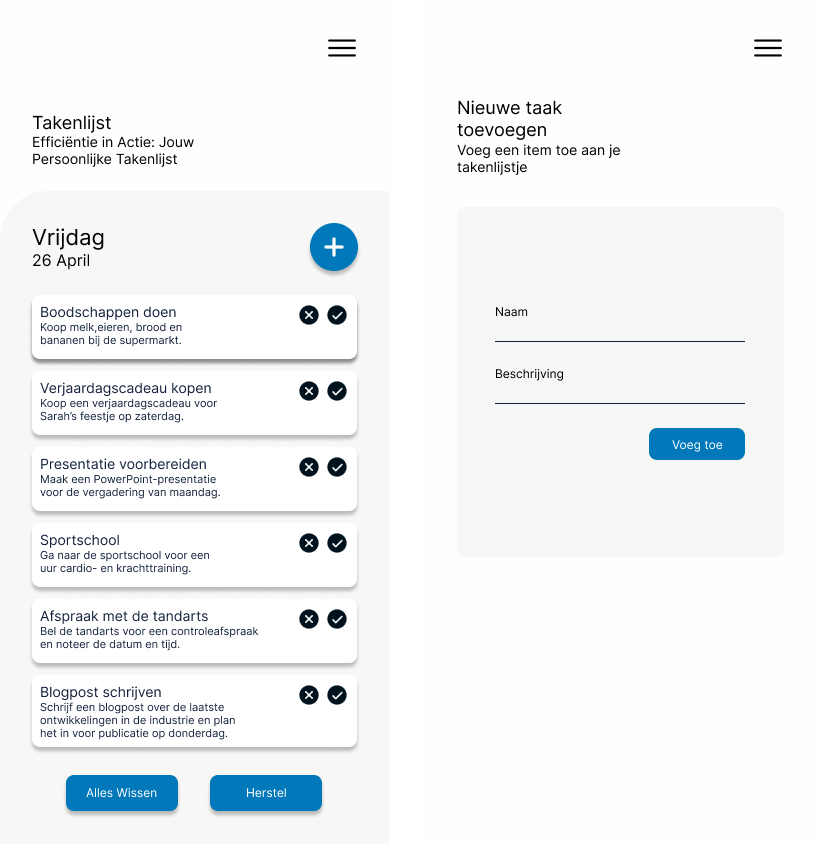
\includegraphics[scale=0.4]{todo_app_poc.png}
\\
Bron - Joeri Verhelst 
\\
\\
Daarbij zal een programmeur een andere app maken, genaamd een feedback app, die bestaat uit een formulier voor feedback dat data opslaat in AirTable.
Vervolgens zal ook via MAKE.com een e-mail gestuurd worden naar de gebruiker die feedback heeft gegeven.
Dit zorgt ervoor dat men de integratie met zowel AirTable als MAKE.com kan testen. Daarnaast zal de applicatie ook een lijst bevatten van alle feedback.
Hieronder bevindt zich ook een ontwerp van de applicatie als leidraad.
\\
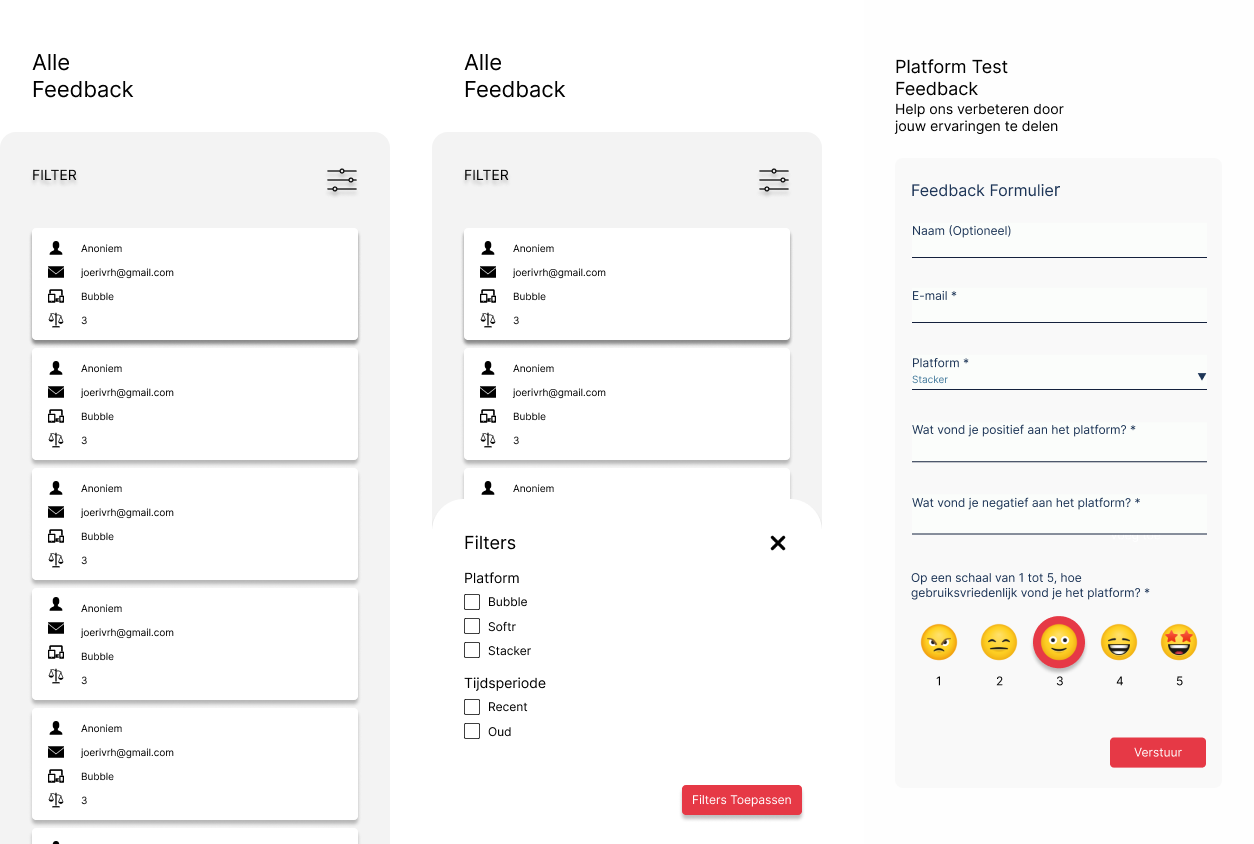
\includegraphics[scale=0.4]{feedback_app_poc.png}
\\
Bron - Joeri Verhelst 
\\
\\
Het is \textbf{belangrijk} om te vermelden dat, door de kleine steekproef, de uitgevoerde Proof of Concept niet voldoende is om een 
definitieve beslissing te nemen over welk platform het beste is voor Quivvy Solutions.

\subsection{Benodigdheden}%
\label{subsec:benodigdheden}
Omdat alle platformen cloud-based zijn, is er een laptop en een internetverbinding nodig om de Proof of Concept uit te voeren. Vervolgens heb je ook 
een account nodig op de drie platformen; Softr, Stacker en Bubble. Deze drie platformen bieden dan ook een gratis versie aan waardoor er geen kosten aan verbonden zijn. Vervolgens zal je ook 
nog een account nodig hebben op AirTable en MAKE.com die ook een gratis versie aanbieden.

\subsection{Uitvoer van de Proof of Concept}%
\label{subsec:uitvoer-proof-of-concept}

\subsubsection{Programmeur}%
\label{subsubsec:programmeur}
Voor de drie platformen te laten testen door een programmeur zal natuurlijk niet alle 3 de platformen tegelijkertijd 
kunnen getest worden, daarom zal de programmeur eerst beginnen met Softr. 
Zoals eerder vermeld zal de programmeur een feedback app moeten maken.
\\
\\
\textbf{1. Softr}
\\
Hiervoor moet hij eerst een account maken op Softr en op AirTable om de app te kunnen maken. 
Daarna kom je terecht op een overzichtelijke dashboard waar je de keuze hebt om templates te kiezen maar 
ook je eigen app te maken van nul of met AI. Bij het ontwikkelen van de app ervaarden de programmeur één probleem. 
Dit probleem was een error dat hij kreeg bij het snel verwijderen van componenten waardoor de pagina zich herstartte. 
Vervolgens merkte hij op dat de app kan hersteld worden aan de hand van de App History waarbij je terug kunt gaan 
naar een bepaalde snapshot. De programmeur heeft dan uiteindelijk de feedback app 
kunnen maken in exact 41 minuten en 54 seconden, de besteden tijd in AirTable is niet inbegrepen. 
Dit was zonder het gebruik van de AI, die Softr aanbiedt om je pagina’s voor u te maken. Vervolgens vond 
de programmeur de aantal integraties dat hij zag redelijk gelimiteerd maar de integratie met Airtable was 
zeer goed en simpel. Je kon wel helaas geen twee tabellen van de database connecteren op 1 formulier. 
Ook zag het er zeer eenvoudig uit om MAKE.com te gebruiken, maar doordat je in Softr geen 2 verschillende connecties 
kan leggen op één knop heeft de programmeur enkel AirTable gebruikt.
\\
\\
Hieronder zie je de AirTable database dat de programmeur heeft gemaakt en hoe het gebruikmaken van AirTable in Softr plaatsnam.
\\
\\
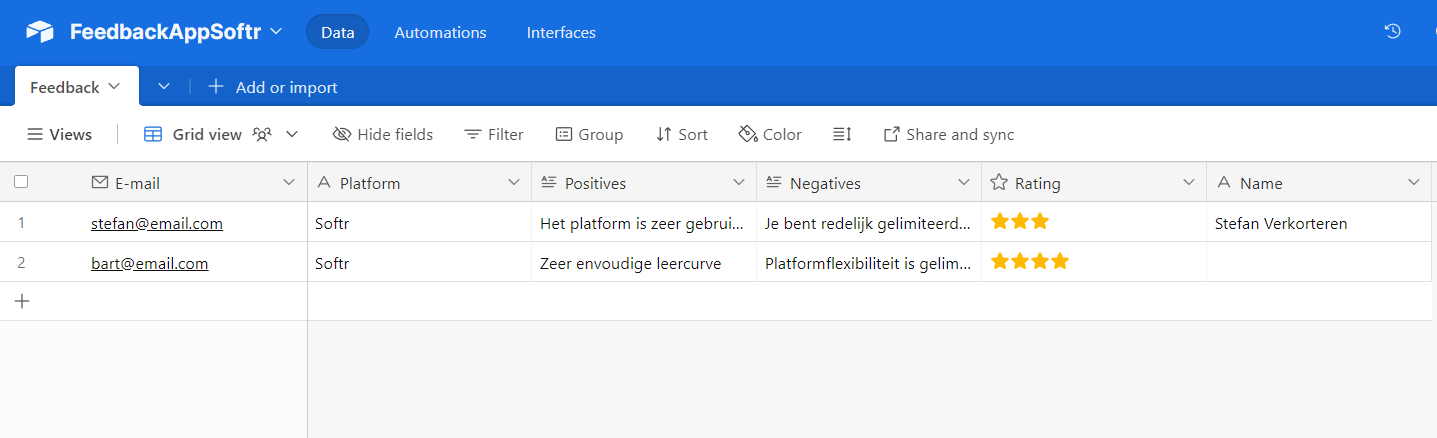
\includegraphics[scale=0.5]{softr/database-airtable-softr.png}
\\
\\
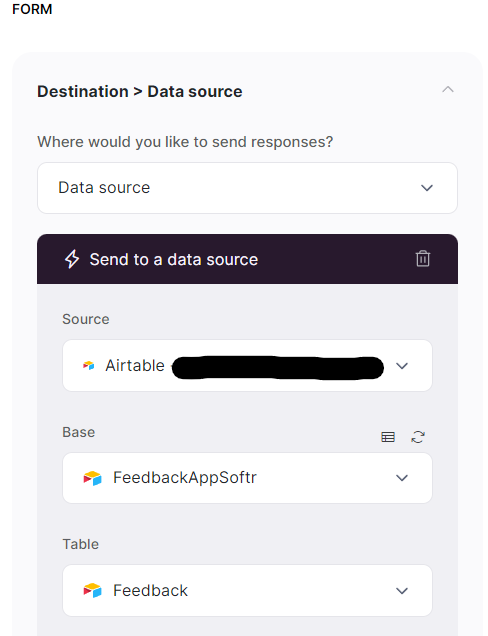
\includegraphics[scale=0.5]{softr/airtable-connectie.png}
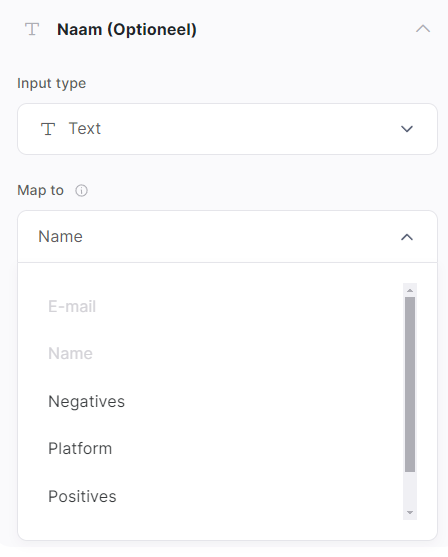
\includegraphics[scale=0.5]{softr/connectie-leggen-aan-airtable-velden.png}
\\
\\
Op vlak van platformflexibiliteit vond de programmeur het zeer matig. 
Want je kan namelijk geen meerdere acties plaatsen op een knop. 
Daarbij is het layout aanpassen van een componenten ook zeer beperkt zoals een component een border radius of shaduw geven is niet mogelijk. 
Wat de programmeur wel zeer tof vond is dat je de optie hebt om eigen custom componenten te maken via high-code en ook templates kon gebruiken.
\\
\\
Softr scoorde wel heel goed op gebruiksvriendelijkheid volgens de programmeur. 
Hij vond het zeer overzichtelijk en kon er snel mee omgaan. 
Juist was het niet mogelijk om individuele delen van een component aan te duiden om snel aan te passen. 
Alle wijzingen moeten namelijk gebeuren in het rechterpaneel waardoor je telkens moest zoeken naar het deel dat je wou aanpassen. 
Ook was je verplicht om een één template aan te duiden als startpagina bij het kiezen om een app te maken van nul, wat zeer apart was. 
\\
\\
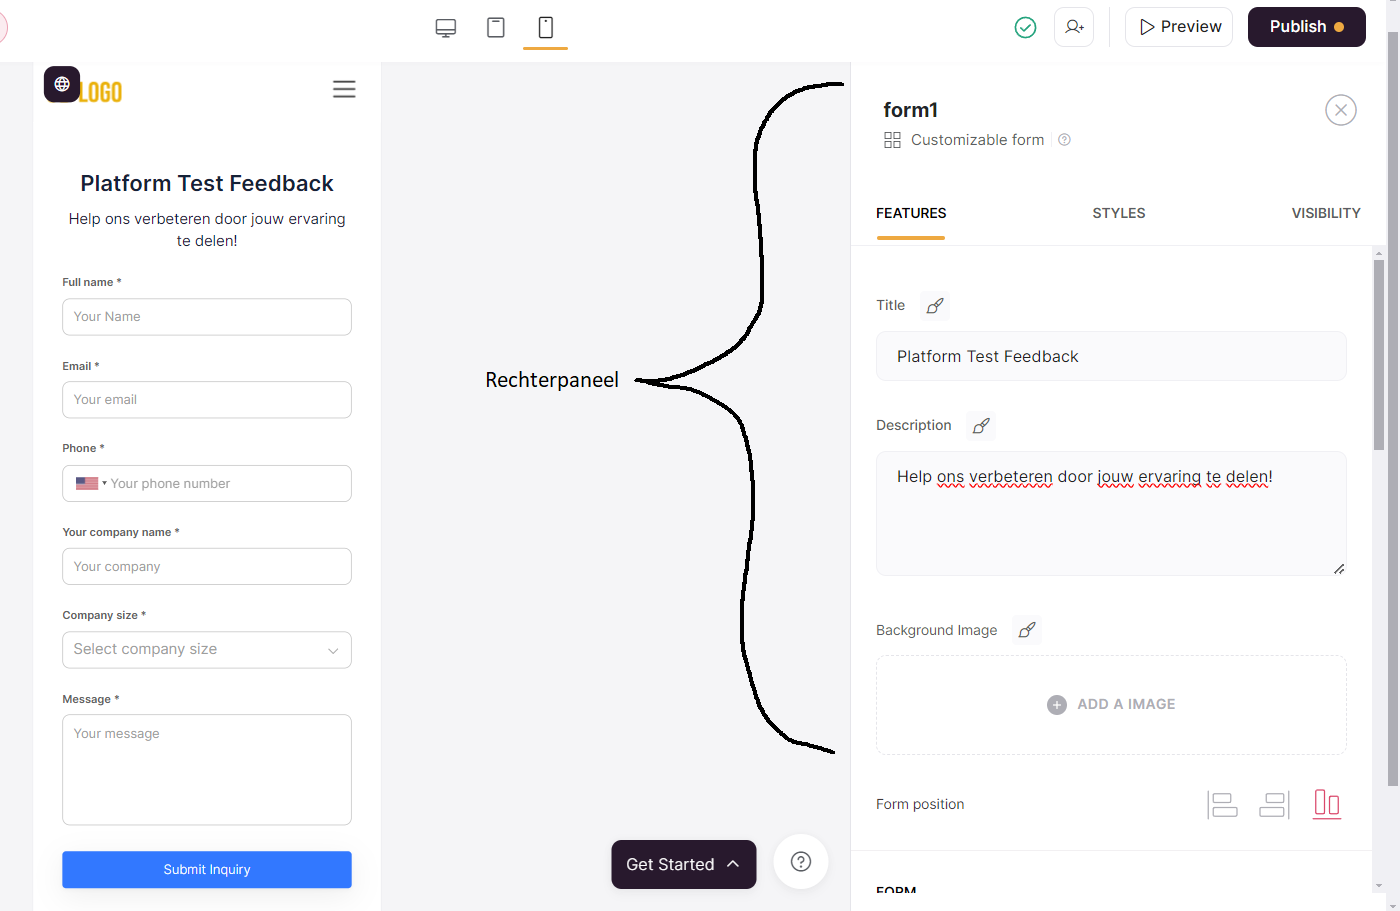
\includegraphics[scale=0.5]{softr/rechter-paneel.png}
\paragraph*{Eindresultaat}
Hieronder kunt u het eindresultaat zien van de feedback app dat gemaakt is in Softr. Door de beperkte platformflexibiliteit kon men namelijk het voorbeeld niet volledig namaken. 
Vervolgens is er ook gebruik gemaakt van een eigen component voor de titel en ondertitel. Dit component werd geschreven in HTML5 met Bootstrap.
\\
\\
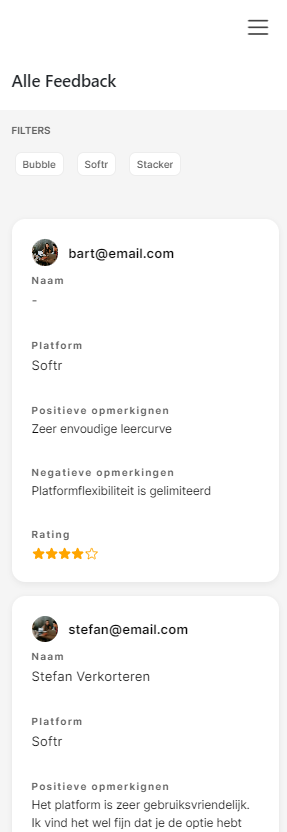
\includegraphics[scale=0.75]{softr/feedbacklijst-softr.png}
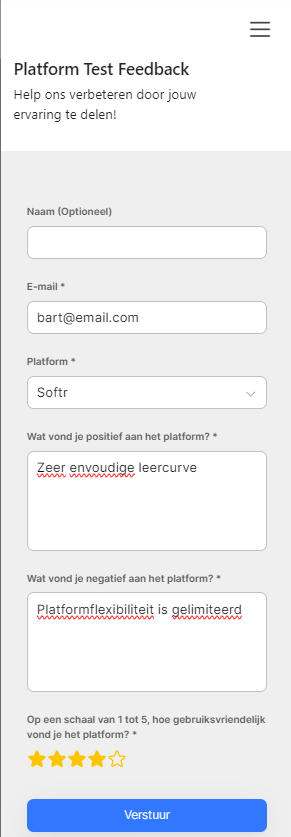
\includegraphics[scale=0.75]{softr/formulier-gemaakt-softr.png}
\paragraph*{Beoordeling}
De programmeur geeft deze app een score van 4 op 5 doordat je kon opmerken dat het platform wel redelijk gelimiteerd is, maar wel de mogelijkheid had om eigen componeten te maken. 
Hierdoor kon de programmeur achterhalen dat het maken complexe apps een echte uitdaging zou zijn met Softr, 
door de beperkte platformflexibiliteit.
\\
\\
\textbf{2. Bubble}
\\
Bij Bubble was het maken en starten van een app gelijkaardig aan Softr. Het platform op zich was snel en vlot om mee te werken. Maar bij het testen van een actie op een knop
kon het proces soms eventjes duren vooraleer de actie werd uitgevoerd. Vervolgens was het wel mogelijk bij bubble om op een knop meerdere acties te plaatsen waardoor men ook 
bij dit platform een mail versturen naar de gebruiker die feedback heeft gegeven. Hieronder kunt u dan ook de scenario vinden dat gemaakt is in MAKE.com.
\\
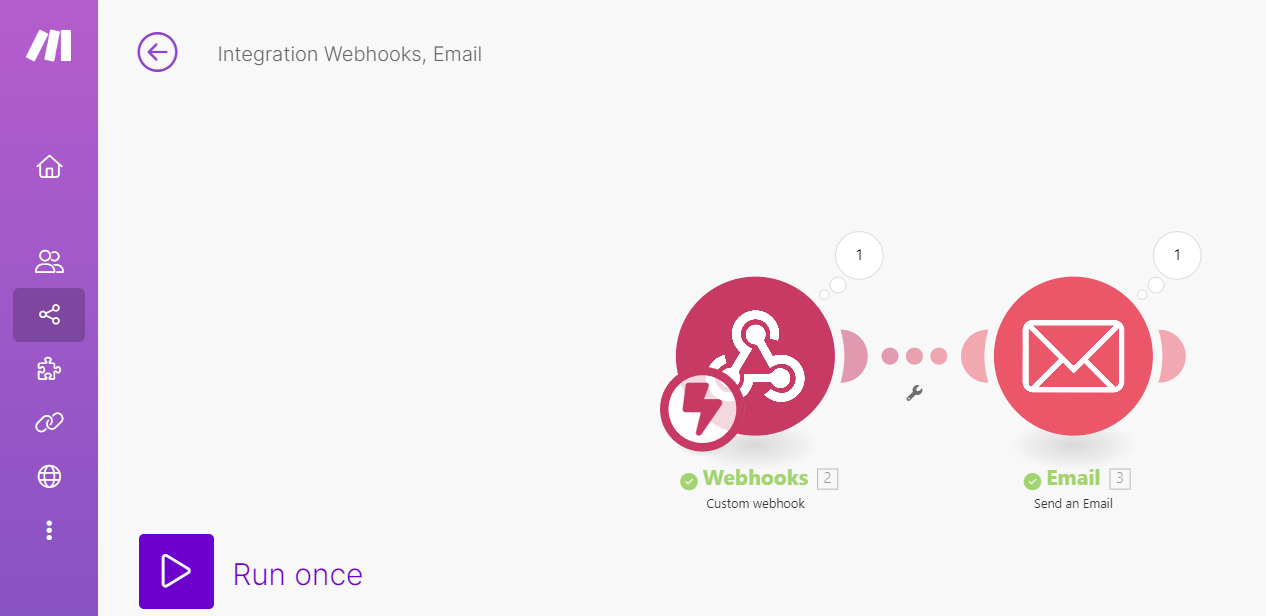
\includegraphics[scale=0.5]{bubble/make-scenario.png}
\\
\\
Het integreren met Airtable en MAKE.com was in het begin zeer verwarrend voor de programmeur. Het duurde toch wel eventjes vooraleer hij doorhad hoe hij de connectie moest leggen.
Na het zoeken naar de documentatie was het duidelijk dat je een personal acces token moet maken op Airtable om dit dan te gebruiken in Bubble. De tijd dat de programmeur nodig had 
om te integreren was 36 minuten en 3 seconden. Hieronder vind u dan ook de AirTable database dat de programmeur heeft gemaakt en de integratie met Bubble.
\\
\\
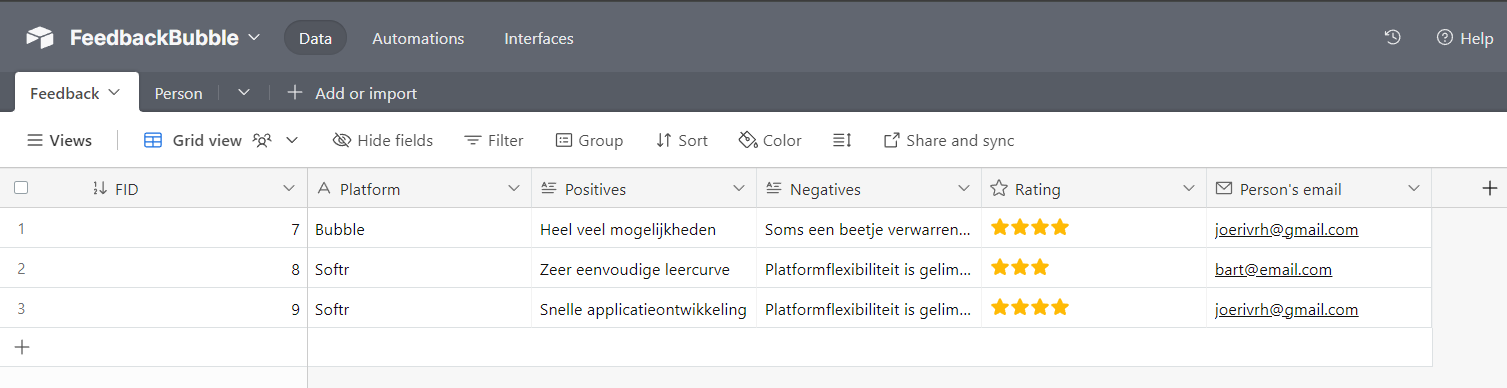
\includegraphics[scale=0.5]{bubble/AirTable-Bubble.png}
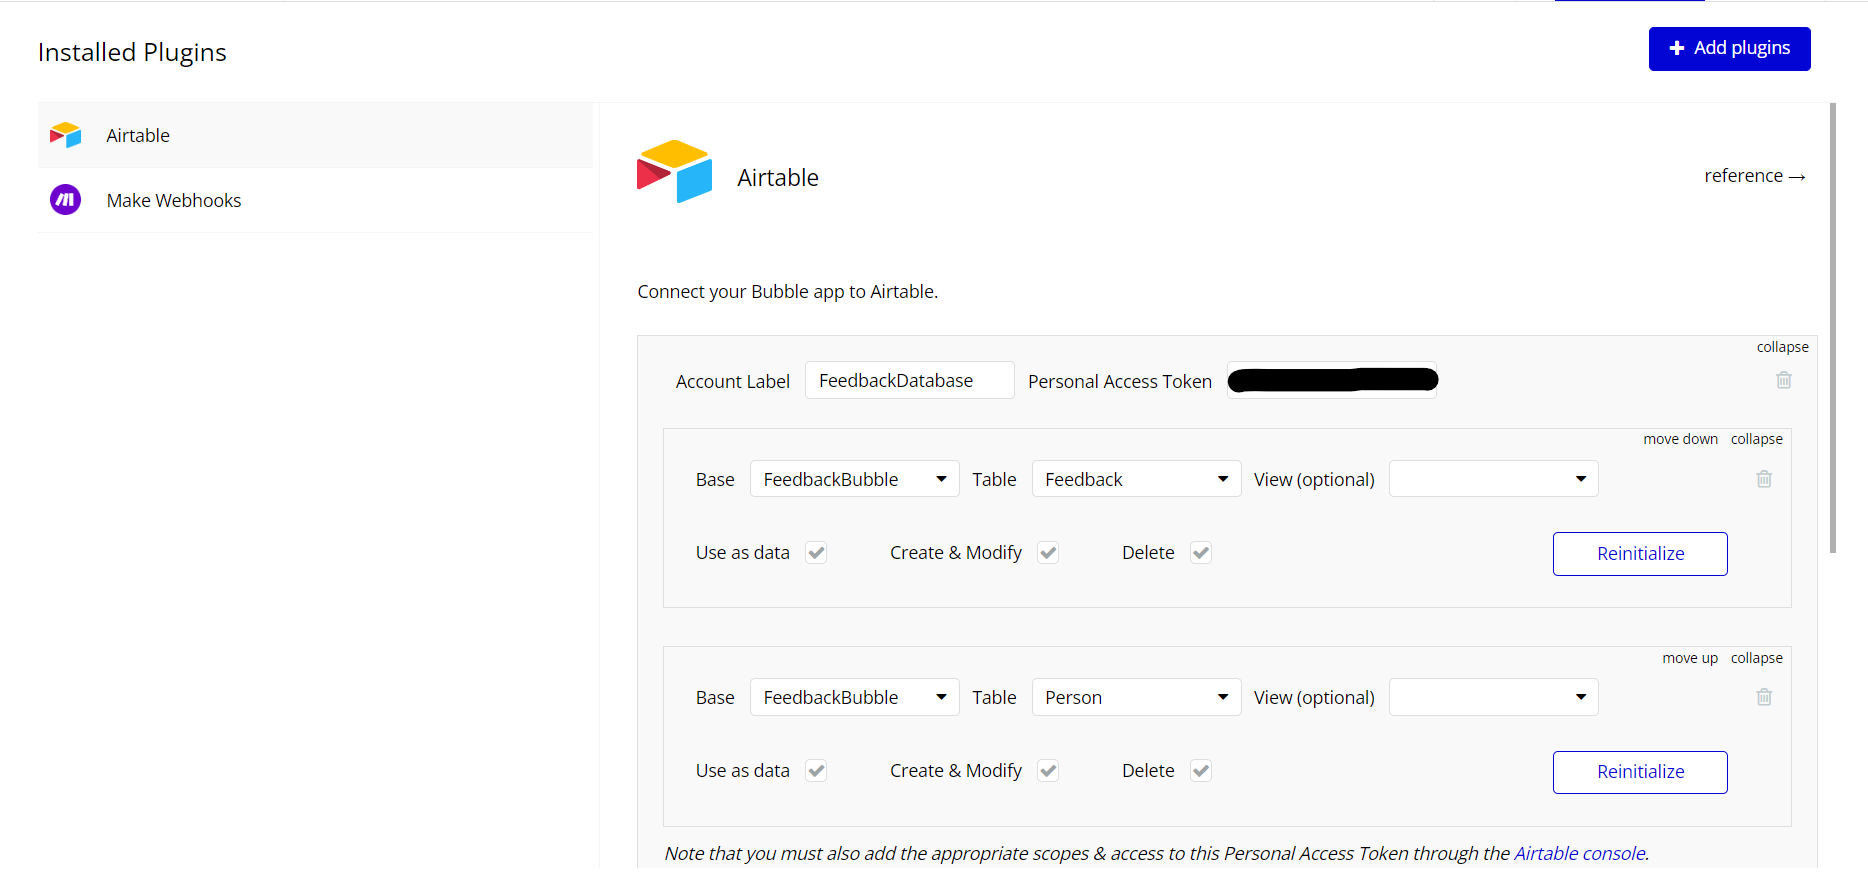
\includegraphics[scale=0.4]{bubble/integratie-airtable.png}
\\
\\
Op vlak van platformflexibiliteit was Bubble zeer goed. Je kon namelijk alles aanpassen van een component zoals de border radius, schaduw, kleur, enzovoort. 
De programmeur vond het ook duidelijk dat je met dit platform complexe apps zou kunnen maken. Daarnaast was het eerst zoeken naar hoe je acties moest plaatsen op een knop.
Je moet namelijk naar een aparte sectie gaan die alle bedrijfslogica bevat. Dit was eerst wat verwarrend voor de programmeur. De flow's of meer specifiek de acties dat je bijvoorbeeld kan doen op een 
knop was zeer flexibel, want dit zorgde ervoor dat je op een knop zowel een actie kan doen met Airtable als met MAKE.com.
\\
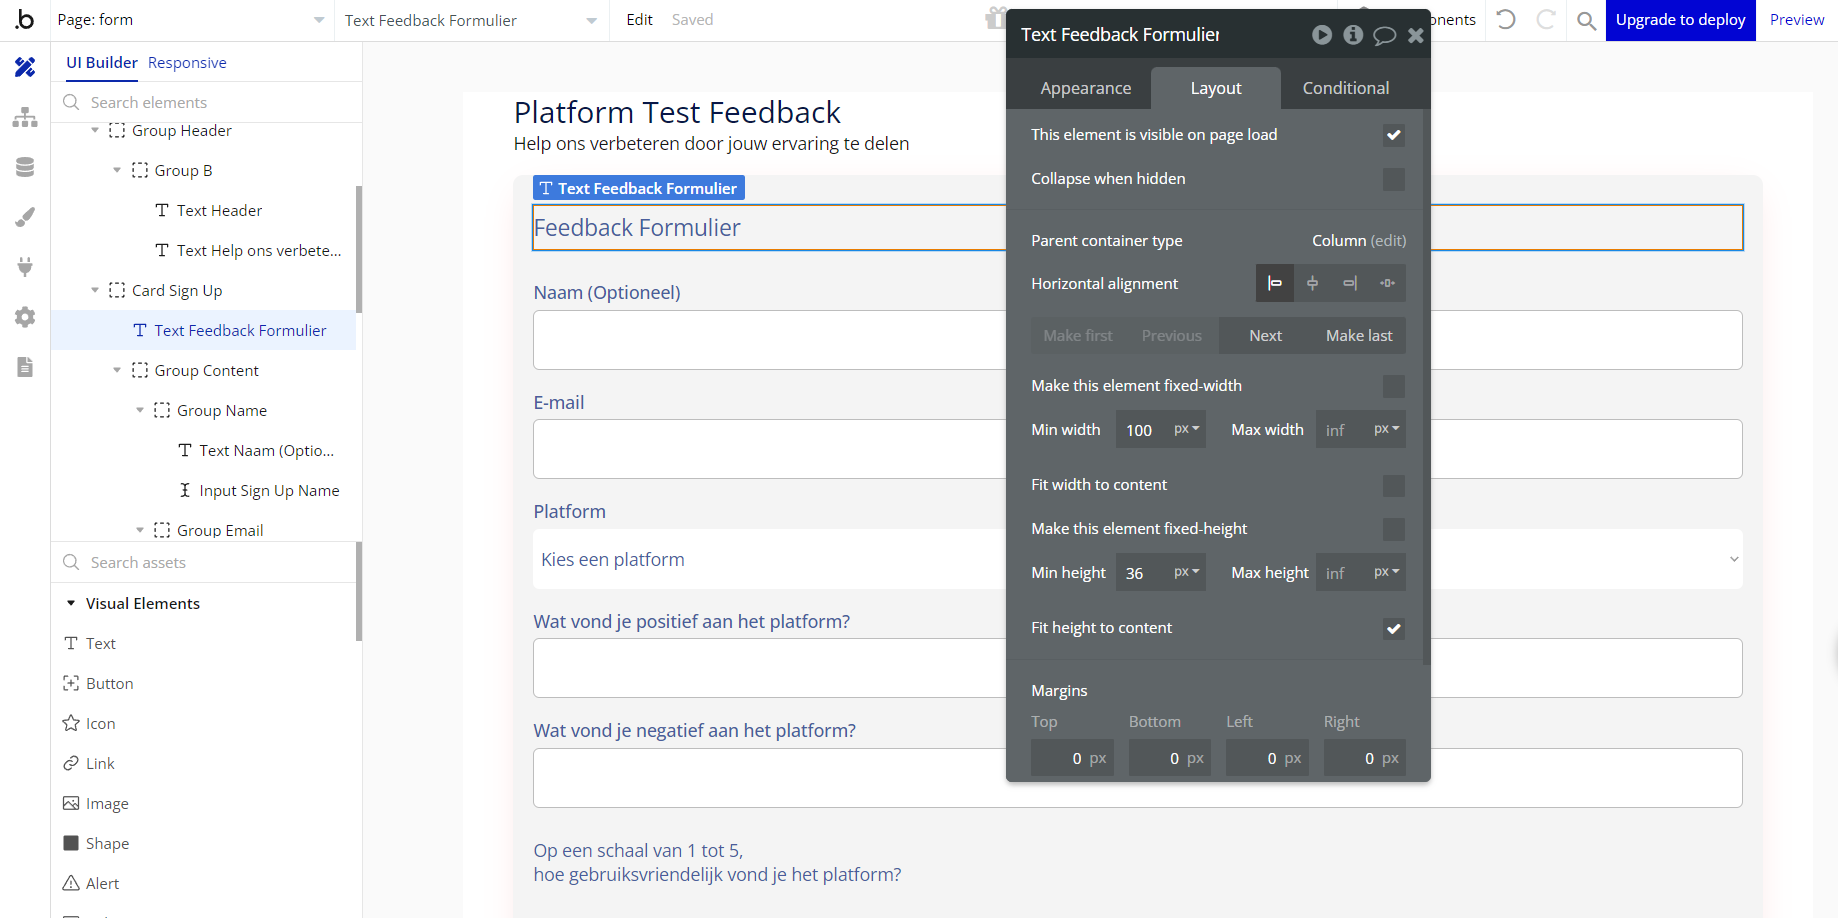
\includegraphics[scale=0.4]{bubble/element-details.png}
\\
\\
De gebruiksvriendelijkheid van de app is goed. Je komt namelijk terecht
op een scherm waarbij je kan kiezen om een app te ontwikkelen via AI of zelf van nul te beginnen. 
Vervolgens heb je de optie om direct plugins te intalleren zoals MAKE.com en Airtable. Daarna moet je de kleuren kiezen van de app.
Bij het klikken op een component krijg je direct de opties te zien die je kan aanpassen, wat zeer handig is want dit geldt voor ook delen in het component. Helaas 
kan je de live data wel niet zien in de editor maar wel bij het previewen van de app.
\\
\\
\paragraph*{Eindresultaat}
De programmeur heeft de app kunnen maken in 1 uur en 52 minutren. De oorzaak hiervan was omdat het vaak wel zoeken was hoe iets in elkaar zat, dit gelde ook bij het integreren van plugins.
Het maken van de feedbacklijst duurde het langste, namelijk 45 minuten en 18 seconden doordat het niet duidelijk was hoe je de data van Airtable moest tonen in een lijst.
Uiteindelijk is de app dat gemaakt is in Bubble zeer gelijkaardig aan het voorbeeld, door de vrijheid die Bubble beschikt. Hieronder vind u dan ook het eindresultaat van de feedback app.
\\
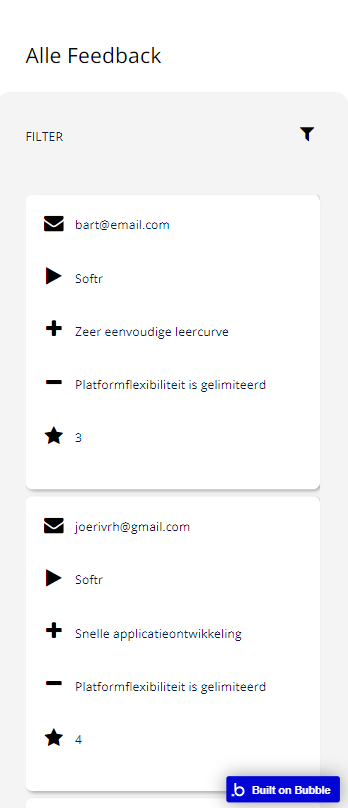
\includegraphics[scale=0.5]{bubble/feedback-lijst-bubble.png}
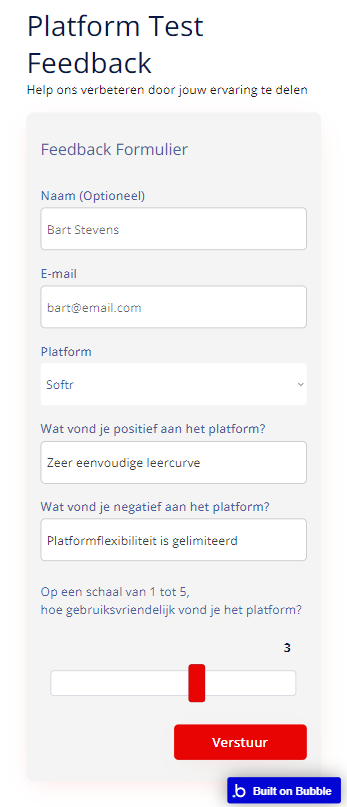
\includegraphics[scale=0.5]{bubble/formulier-resultaat-bubble.png}
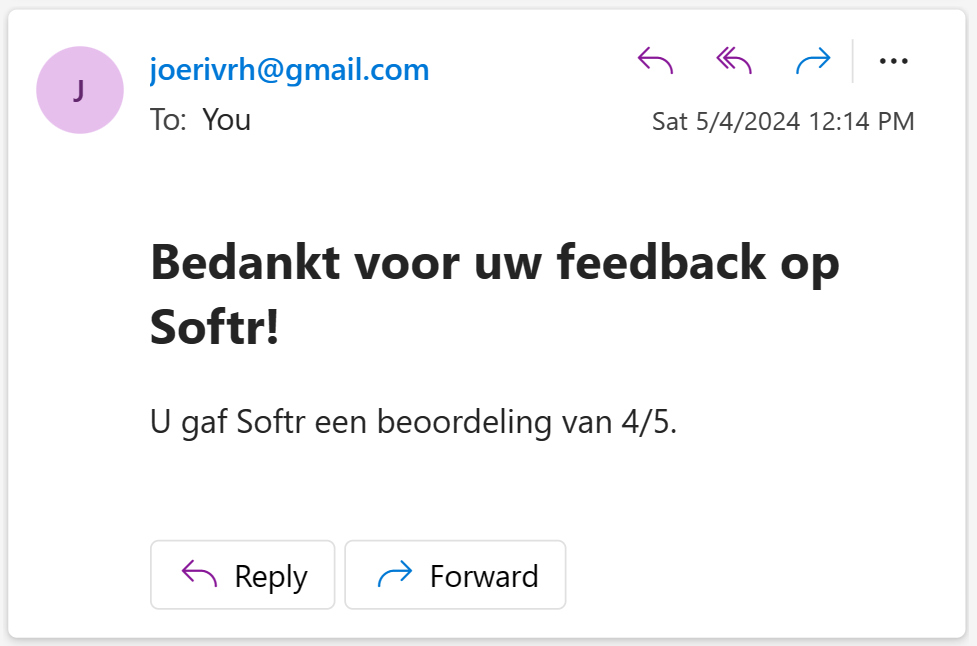
\includegraphics[scale=0.5]{bubble/ontvangen-email-bij-formulier-bubble.png}
\paragraph*{Beoordeling}
De beoordeling dat deze app heeft gekregen is 4.5 op 5. Dit komt omdat het platform zeer flexibel is. 
De beoordeling was net geen 5 op 5 omdat het soms wel zoeken was hoe je iets moest doen.
\\
\\
\textbf{3. Stacker}
\\
Bij Stacker was het proces voor het maken van een app zeer strikt en kon je niet veel aanpassen. Je moest namelijk eerst een account maken met een bedrijfsaccount.
Daarna werd er direct gevraagd om een databron te connecteren met Stacker. Hiervoor nam de programmeur AirTable waarbij het connecteren zeer snel en vlot verliep, door de duidelijke documentatie.
Helaas merkte de programmeur op, bij het ontwikkelen van de feedback app, dat het niet mogelijk was om MAKE.com te integreren met Stacker.
\\
\\
Hieronder zie je de AirTable database dat de programmeur heeft gemaakt.
\\
\\
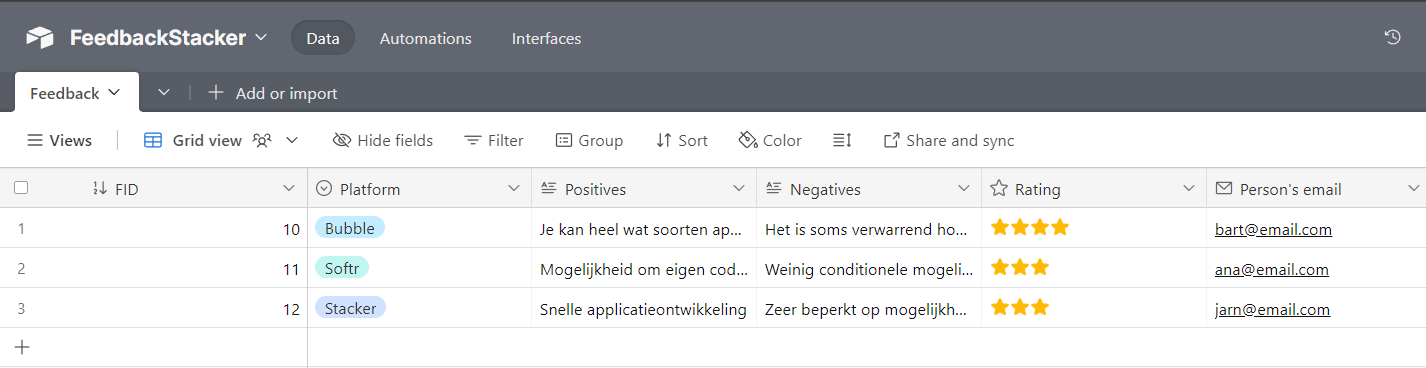
\includegraphics[scale=0.5]{stacker/airtable_stacker.png}
\\
Op vlak van platformflexibiliteit had je heel weinig vrijheid om je app aan te passen. Je kon namelijk niet de kleur kiezen van componenten want de kleuren worden gekozen
op basis van je bedrijfskleur. Daarnaast heb je ook weinig keuze in componenten. De programmeur vond dat dit platform meer bedoelt is voor het maken van CRM's en portals in plaats van 
mobiele of complexe apps.
\\
\\
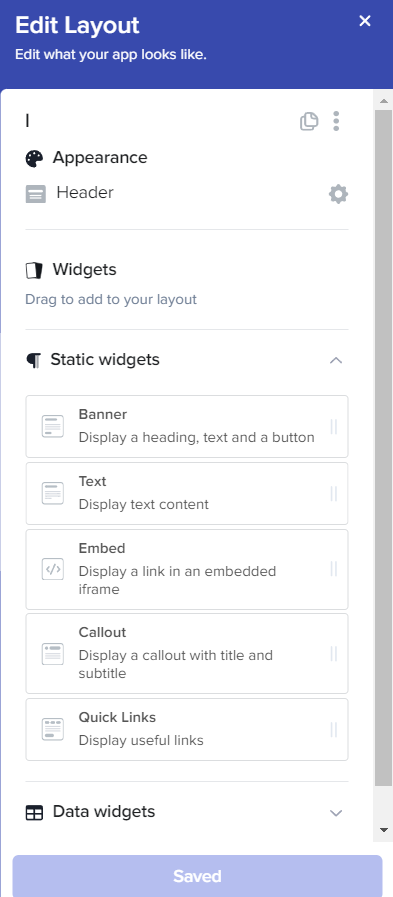
\includegraphics[scale=0.5]{stacker/componenten-stacker1.png}
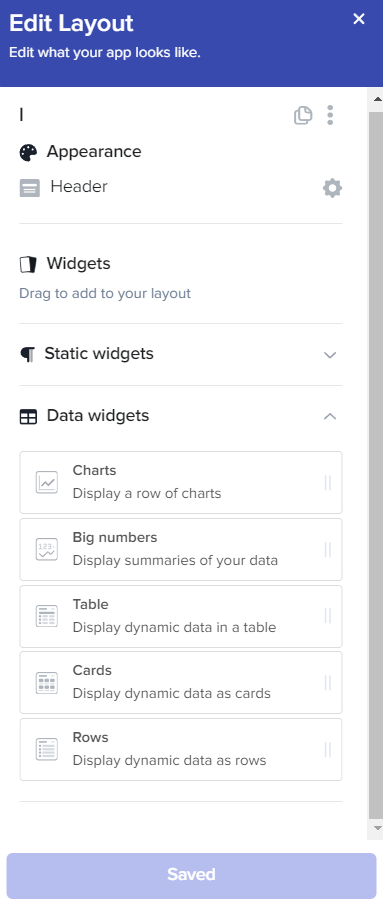
\includegraphics[scale=0.5]{stacker/componenten-stacker2.png}
\\
De programmeur vond Stacker gebruiksvriendelijk op bepaalde vlakken. Zo was het connecteren met AirTable zeer eenvoudig en duidelijk.
Ook was het leren van het platform eenvoudig door de duidelijke user interface. Maar in eerste instantie was het wel wat verwarrend om te weten waar je moest beginnen.
Het was namelijk zo dat hij niet wist of dat hij al op het scherm zat voor een app te maken of niet omdat je automatisch al een navigatiebalk hebt.
\\
\\
\paragraph*{Eindresultaat}
Door de zeer beperkte platformflexibiliteit was het namaken van het voorbeeld een grote uitdaging. Hierdoor is het namaken niet gelukt maar hij heeft wel een formulier en homescherm
kunnen ontwikkelen. Tijdens het ontwikkelen was het platform redelijk snel maar de programmeur ervaarden een crash van de laptop bij het snel klikken van verschillende knoppen op het platform.
Deze crash duurde ook ongeveer 30 seconden vooraleer alles terug normaal was. Het totaal ontwikkelen van de app heeft 26 minuten en 47 seconden geduurd. Waarbij het connecteren met AirTable 4 minuten 23 seconden duurde, het ontwikkelen van het formulier 16 minuten en 46,
en het maken van het homescherm 5 minuten en 38 seconden. Hieronder vind u dan ook het eindresultaat van de feedback app.
\\
\\
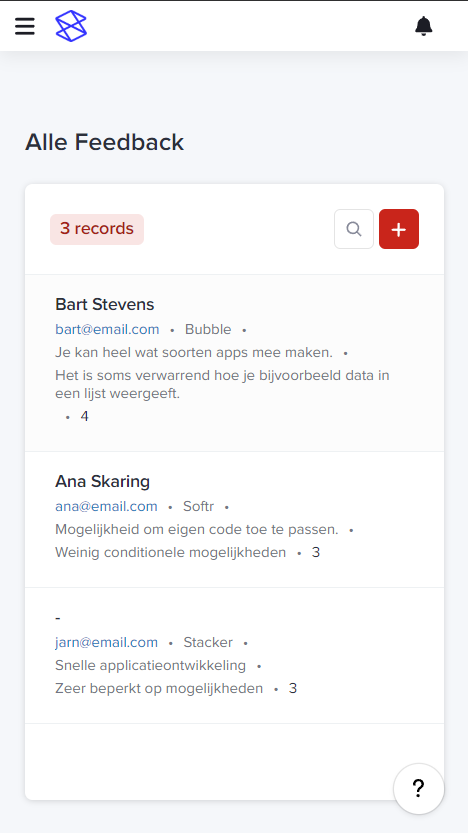
\includegraphics[scale=0.75]{stacker/feedback_lijst.png}
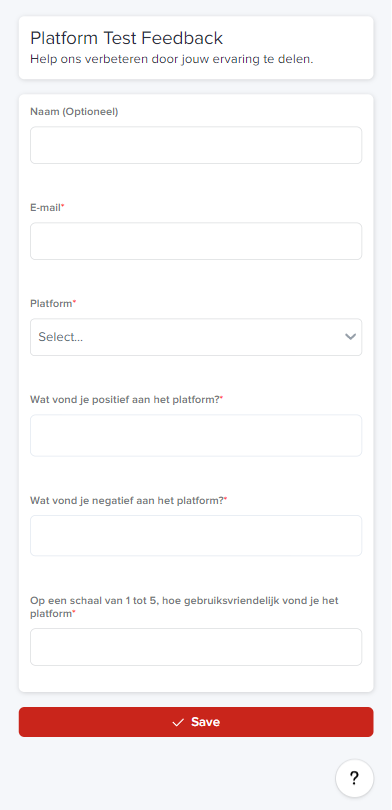
\includegraphics[scale=0.75]{stacker/formulier.png}

\paragraph*{Beoordeling}
Door de zeer matige platformflexibiliteit en de beperkte mogelijkheden van apps maken geeft de programmeur Stacker een score van 3 op 5.
De programmeur beveelden dit platform niet aan voor complexe apps te maken, maar eerder voor CRM's en portals.

\subsubsection{Niet-programmeurs}%
\label{subsubsec:niet-programmeurs}
De Proof of Concept voor niet programmeurs, die geen ervaring hebben met programmeren of IT, werd uitgevoerd om 
de gebruiksvriendelijkheid van de platformen te testen. Ter info, deze Proof of Concept is zeer beperkt en is niet voldoende om een definitieve beslissing te nemen over welk platform het beste ervaring geeft voor niet-programmeurs.
\\
\\
\textbf{1. Bubble}
\\
De twee participanten voor Bubble waren Jonas en Marleen. Jonas is begonnen met Bubble als eerste platform waarbij het ongeveer 1u en 25 minuten duurde om de app te maken.
Voor zijn eerste ervaring met zowel een No-Code platform als het platform Bubble vond hij het platform verwarrend. Vervolgens vond hij het gebruiksvriendelijkheid acceptabel doordat het soms
wel zoeken was hoe je iets moest doen. Daarnaast vond hij dat het platform u wel veel mogelijkheden gaf om je app te maken en aan te passen, dit was een reden waarom het juist wat verwarrend was voor hem.
Ten slotte gaf hij het platform een score van 4 op 5 voor hoe goed zijn ervaring was met het platform.
\\
\\
Marleen ondervond verschillende uitdagingen bij het maken van een app in Bubble waarbij zowel de logica als elementen aanpassen moeilijk ging. Hierdoor moest de organisator
regelmatig helpen bij het maken van de app, die ze in ongeveer 1 uur en 30 minuten heeft gemaakt. Ze vond wel dat het platform gebruiksvriendelijk is met hulp maar zonder hulp zou dit niet zo zijn. Ze vond wel een paar dingen positief zoals de vele elemeten die ze kon aanpassen. Daarbij merkte ze ook op 
dat dit platform veel meer biedt dan Stacker. Het enigste waar Marleen niet tevreden overe was het implementeren van logica in de app. Ten slotte gaf ze het platform een score van 2.5 op 5 voor hoe goed haar ervaring was met het platform.
\\
\\
\textbf{2. Softr}
\\
Er waren twee participanten die Softr hebben uitgestest, namelijk Jonas en Ronny. Ronny die begonnen is met Softr als platform heeft een soortgelijke app
gemaakt in ongeveer 1 uur en 15 minuten. Hieruit volgt dat hij meedeelde dat de meeste delen van het platform op eerste instantie niet duidelijk was, maar naarmate de tijd
ging werd het duidelijker. Vervolgens vond hij het platform wel gebruiksvriendelijk waarbij het aanpassen van de indeling zoals kleuren aanpassen zeer eenvoudig was om te toe te passen. Vervolgens heeft Ronny
heel wat moeten vragen aan de organisator.
Ten slotte gaf hij het platform een score van 4 op 5 voor hoe goed zijn ervaring was met het platform.
\\
\\
Jonas heeft voor zijn tweede platform Softr mogen uittesten. In dit platform heeft hij ongeveer 45 minuten gespendeerd om grotendeels de app te kunnen namaken.
Hij vond dat grotendeels alles duidelijk was maar het was soms wel een beetje zoeken. Vervolgens informeerde hij dat het platform gebruiksvriendelijk is, want hij vond het namelijk gemakkelijk om
een vóór opgemaakt lijst of formulier aan te passen naar zijn eigen stijl. Daarbij was er niks negatief aan het platform waardoor hij een score gaf van 5 op 5.
\\
\\
\textbf{3. Stacker}
\\
De participanten voor Stacker waren Ronny en Marleen. Marleen die begonnen is met Stacker als platform heeft ongeveer 1 uur  gespendeerd om de app te proberen namaken, waarbij de organisator regelmatig moest ingrijpen.
In het begin was het moeilijk om te begrijpen voor haar, maar naargelang ze ermee werkte werd het beter. Hieruit volgt dat ze de gebruiksvriendelijkheid niet zo top vond maar vertelde dat het beter zou zijn als ze meer tijd had om het platform te leren kennen.
Ten slotte gaf ze het platform een score van 3 op 5 voor hoe goed haar ervaring was met het platform.
\\
\\
Ronny heeft voor zijn tweede platform Stacker mogen uittesten. In dit platform heeft hij ongeveer 30 minuten gespendeerd om de app te proberen namaken, waarbij de organisator soms moest helpen.
Na een tijdje begon hij het platform beter te begrijpen en vond hij het platform wel gebruiksvriendelijk. Hij vond het namelijk eenvoudig en overzichtelijk om te gebruiken. Ten slotte was zijn ervaring een 
score van 4 op 5 op het platform.
% Voeg hier je eigen hoofdstukken toe die de ``corpus'' van je bachelorproef
% vormen. De structuur en titels hangen af van je eigen onderzoek. Je kan bv.
% elke fase in je onderzoek in een apart hoofdstuk bespreken.

%\input{...}
%\input{...}
%...

%%=============================================================================
%% Conclusie
%%=============================================================================

\chapter{Conclusie}%
\label{ch:conclusie}

% TODO: Trek een duidelijke conclusie, in de vorm van een antwoord op de
% onderzoeksvra(a)g(en). Wat was jouw bijdrage aan het onderzoeksdomein en
% hoe biedt dit meerwaarde aan het vakgebied/doelgroep? 
% Reflecteer kritisch over het resultaat. In Engelse teksten wordt deze sectie
% ``Discussion'' genoemd. Had je deze uitkomst verwacht? Zijn er zaken die nog
% niet duidelijk zijn?
% Heeft het onderzoek geleid tot nieuwe vragen die uitnodigen tot verder 
%onderzoek?
Als men terug blikt op de vraag die gesteld werd in de inleiding: welk platform het meest geschikt is voor Quivvy Solutions, had men verwacht dat het Softr zou zijn. Maar men kan concluderen dat Bubble beter zou passen bij het bedrijf. 
Deze conclusie heeft men kunnen trekken door de zeer uitgebreide methodologie; alternatieven, vergelijkende analyse, en Proof of Concept. De reden dat Bubble aangeraden wordt, is omdat het voor Quivvy Solutions noodzakelijk is dat het platform
kan integreren met zowel AirTable als MAKE.com. Bubble heeft deze mogelijkheden en heeft ook een groot aantal plugins. Daarnaast is Bubble ook superieur bij het gebruik van diverse databases en platformflexibiliteit.
Vervolgens is Bubble stabieler op lange termijn en interessanter voor grote bedrijven. De prijs van Bubble is tegenover de twee andere platformen minder duur. Het platform is ook veel transparanter naar hun 
gebruikers toe op het vlak van updatebeleid. De enigste minpunten van Bubble is dat Softr en Stacker beter scoorde op snelheid van applicatieontwikkeling en gebruiksvriendelijkheid. Helaas weten we niet hoe goed elke platform is bij het maken
van complexe apps. Dit omdat we enkel een Proof of Concept hebben gemaakt waarin simpele applicaties werden gebouwd. We kunnen concluderen dat volgens de programmeur van de Proof of Concept Softr en Stacker minder geschikt zou zijn voor complexe apps. Hieruit volgt dat men verder kan onderzoeken 
hoe deze platformen presteren bij het maken van complexe apps. Ten slotte is het belangrijk om te vermelden dat de uitgevoerde Proof of Concept niet voldoende is om een definitieve beslissing te nemen.




%---------- Bijlagen -----------------------------------------------------------

\appendix

\chapter{Onderzoeksvoorstel}

Het onderwerp van deze bachelorproef is gebaseerd op een onderzoeksvoorstel dat vooraf werd beoordeeld door de promotor. Dat voorstel is opgenomen in deze bijlage.

%% TODO: 
%\section*{Samenvatting}

% Kopieer en plak hier de samenvatting (abstract) van je onderzoeksvoorstel.

% Verwijzing naar het bestand met de inhoud van het onderzoeksvoorstel
%---------- Inleiding ---------------------------------------------------------

\section{Introductie}%
\label{sec:introductie}

Bedrijven aarsen op effeciëntie, kosten  verminderen, en veiligheid. Dit is niets anders dan ook bij het softwarebedrijf genaamd Quivvy waarbij de trend No-Code en Low-Code
platforms voor het bouwen van applicaties de laatste jaren rond dwaalt. Momenteel gebruikt Quivvy FlutterFlow voor het bouwen van Mobile \& Web Portals. 
Hierbij interageert FlutterFlow met AirTable, een database platform. Maar bedrijven zijn voortdurend op zoek naar de beste softwareplatformen om hun bedrijf te runnen.
Daarom zoekt Quivvy naar een alternatief voor het bouwen van Mobile \& Web Portals dat zowel goed werkt voor bedrijf als eindklant, maar ook interageert met AirtTable of Podio.
De markt van No-Code en Low-Code platforms worden overspoeld met verschillende platformen waaronder Microsoft PowerApps, Bubble, Webflow, Softr en Stacker.
Als gevolg dat drie op de vier van de grootste bedrijven tegen 2024 gebruik zullen maken van Low-Code platforms ~\autocite{Moskal_2021} ~\autocite{Kulkarni_2021}.
Deze No-Code en Low-Code platforms hebben ook een reden tot de populariteit, namelijk dat
deze platforms het mogelijk maken om applicaties te bouwen zonder enige tot weinig kennis van programmeren. Dit is niet het enige waarom deze platforms een trend zijn,
want het zorgt ook voor een snelle ontwikkeling met lage kosten door de effeciënte gebruik van de ontwikkelaars.
Maar welke bestaande softwareplatform is geschikt voor Mobile \& Web portals te creëren, dat zowel goed werkt voor bedrijf als eindklant?
In deze bachelorproef hanteren we het meest geschikte Mobile \& Web Portals voor een softwarebedrijf en eindklant.
Waarbij we een vergelijking maken tussen Softr en Stacker, beide No-Code en/of Low-Code platforms. Daarbij wordt er rekening gehouden met verschillende 
factoren zoals snelheid, gebruiksvriendelijkheid, enzovoort.


%Waarover zal je bachelorproef gaan? Introduceer het thema en zorg dat volgende zaken zeker duidelijk aanwezig zijn:

% \begin{itemize}
%   \item kaderen thema
%   \item de doelgroep
%   \item de probleemstelling en (centrale) onderzoeksvraag
%   \item de onderzoeksdoelstelling
% \end{itemize}

% Denk er aan: een typische bachelorproef is \textit{toegepast onderzoek}, wat betekent dat je start vanuit een concrete probleemsituatie in bedrijfscontext, een \textbf{casus}. Het is belangrijk om je onderwerp goed af te bakenen: je gaat voor die \textit{ene specifieke probleemsituatie} op zoek naar een goede oplossing, op basis van de huidige kennis in het vakgebied.

% De doelgroep moet ook concreet en duidelijk zijn, dus geen algemene of vaag gedefinieerde groepen zoals \emph{bedrijven}, \emph{developers}, \emph{Vlamingen}, enz. Je richt je in elk geval op it-professionals, een bachelorproef is geen populariserende tekst. Eén specifiek bedrijf (die te maken hebben met een concrete probleemsituatie) is dus beter dan \emph{bedrijven} in het algemeen.

% Formuleer duidelijk de onderzoeksvraag! De begeleiders lezen nog steeds te veel voorstellen waarin we geen onderzoeksvraag terugvinden.

% Schrijf ook iets over de doelstelling. Wat zie je als het concrete eindresultaat van je onderzoek, naast de uitgeschreven scriptie? Is het een proof-of-concept, een rapport met aanbevelingen, \ldots Met welk eindresultaat kan je je bachelorproef als een succes beschouwen?

%---------- Stand van zaken ---------------------------------------------------

\section{State-of-the-art}%
\label{sec:state-of-the-art}

 In de software wereld bevindt men in projecten dat er telkens over het budget wordt gegaan. Daarnaast doet het project meestal niet wat de klant verwacht 
 en vervolgens  doet het opgeleverde product niet wat het moet doen ~\autocite{Moskal_2021}. Volgens ~\textcite{Moskal_2021} zijn deze problemen niet alleen maar te zien in de software wereld, 
 maar ook in andere categorieën binnen de IT-sector, of bij het implementeren en ontwerpen van software systemen. 
 Dit brengt het onderwerp Low-Code en No-Code naar boven ~\autocite{Kulkarni_2021}. 
 Deze platforms zorgen ervoor dat u geen tot weinig kennis nodig heeft over programmeren waardoor deze wordt beschouwt als een trend waar heel wat mensen geïnteresseerd in is ~\autocite{Kulkarni_2021}.
 Maar in vergelijking met andere technologie trends zoals AI, Blockchain, Edge Computing, en RPA groeit LCNC zeer matig in vergelijking met de andere trends ~\autocite{Kulkarni_2021}.
 Toch stijgt het gebruik van No-Code platforms, maar waarom? Dit kan men onderverdelen in vier categorieën:
\begin{itemize}
  \item \textbf{Beperkt aantal programmeurs}: 
  Heel wat studenten laten zich afschrikken door het programmeren. 
  Hierdoor is er kort aantal studenten die werkelijk diepe kennis hebben op vlak van programmeren. 
  Maar het vinden van een zeer gekwalificeerde programmeur brengt projecten niet altijd tot een goed einde ~\autocite{Moskal_2021}.
  \item \textbf{Technologische turbulentie}: De constante evolutie van programmeertalen zorgt ervoor dat de kennis van programmeurs niet altijd de meest recente is  ~\autocite{Moskal_2021}.
  \item \textbf{Hoge kosten}: De traditionele softwareontwikkeling heeft een grote tol op de kosten van een bedrijf. Daarbij beseffen Software engineers dat het bouwen van een applicatie niet gemakklijk is binnen een budget ~\autocite{Moskal_2021}.
  \item \textbf{Tijdrovend}: De traditionele softwareontwikkeling is een tijdrovend proces. De geschatte tijd om Software te maken op één operating systeem is zes maanden of zelfs lange ~\autocite{Moskal_2021}.
  \item \textbf{Complexe softwareontwikkeling}
\end{itemize} 
Het gebruik van het woord No-Code development wordt gezien als een synoniem voor Low-Code development,
daarom kan me verwijzen naar low-code als no-code maar ook omgekeerd ~\autocite{Rokis_2022}. 

\subsection*{LCNC Uitdagingen}
\label{sub:lcnc-uitdagingen}
Om grondig door alle LCNC uitdagingen te gaan, zullen we ze op delen in bepaalde fasen
die gebeuren tijdens het ontwikkelen van een applicatie. 
Deze zijn; requirements analyse, planning, application design, development, testing, deployment, en maintenance ~\autocite{Rokis_2022}.
\subsubsection*{Requirements Analyse}
\label{sub:requirements-analyse}
Doordat specificaties verschilt per platform binnen software, kan dit als een uitdaging worden gezien ~\autocite{Rokis_2022}.
Hierdoor wordt een tool voor eisenbeheer binnen LCNC beschouwd als een waardevolle toevoeging ~\autocite{Rokis_2022}. 
In deze fase wordt veranderingen in de eisen ook gezien als een struikelblok. Maar door het gebruik van LCNC kan dit worden opgelost 
door het gebruik van een prototype, waarbij men steeds de volgende dag snel een oplossing kunnen leveren en onderhouden ~\autocite{Rokis_2022}.
\subsubsection*{Planning}
\label{sub:planning}
In de planning fase komen we terecht bij het kiezen van de meest compatibele LCNC platform die de eisen goed vastneemt ~\autocite{Rokis_2022}.
Volgens ~\textcite{Rokis_2022} maakt de overvloed van de beschikbare platforms op de markt het zeer moeilijk om de meest compatibele te vinden. De 
kosten, leercurve, ondersteuning van functies en functionaliteiten in ontwikkeling spelen allemaal een belangrijke rol ~\autocite{Rokis_2022}. Daarnaast zijn vele
bedrijven bezorgd over "vendor-lock-in". De klant is daarbij sterk afhankelijk van een bepaalde levarancier, waardoor het moeilijk is om over te stappen ~\autocite{Rokis_2022} ~\autocite{Yan2021}.
\subsubsection*{Application Design}
\label{sub:application-design}
De applicatie ontwerp is redelijk gelimmiteerd binnen LCNC.
Ten eerste hebben we te maken met het probleem dat de meeste LCNC platform niet uitbreidbaar zijn ~\autocite{Rokis_2022}.
Als tweede zijn er overwegingen over de betrekking tot schaalbaarheid ~\autocite{Rokis_2022}. 
Vervolgens kan er bepereking zijn op het vlak gegevens opslaan en het ontwerp van de gebruikersinterface ~\autocite{Rokis_2022}.
\subsubsection*{Development}
\label{sub:development}
Bij het ontwikkelen van de software kunnen verschillende uitdagingen voorkomen.
Volgens ~\textcite{Rokis_2022} kunnen in sommige gevallen kan de gelimmiteerde functionaliteit van LCNC platformen een probleem vormen.
Hierdoor moet men dan zelf code schrijven waardoor men meer tijd moeten spenderen en complexiteit toevoegen aan het project ~\autocite{Rokis_2022}.
Daarnaast zouden we ook rekening moeten houden met de moeilijk op het vlak debuggen in een grafische representatie ~\autocite{Rokis_2022}.
\subsubsection*{Maintenance}
\label{sub:maintenance}
Een voordeel van LCNC is dat het onderhoud van de applicatie zeer weinig vraagt ~\autocite{Rokis_2022}.
Volgens ~\textcite{Rokis_2022} komen we hier weer terecht met de uitdaging van debuggen in een grafische representatie.

\subsection*{LCNC binnen bedrijven}
\label{sub:lcnc-binnen-bedrijven}
Verschillende soorten organisaties hangen af van software zodat de organisaties kunnen functioneren ~\autocite{Hintsch2021}.
Volgens ~\textcite{Rafiq_2022} is dit ook het geval bij software start-ups en midden tot grote bedrijven. 
Software start-ups zijn jonge bedrijven met een gelimmiteerd aantal middelen ~\autocite{Rafiq_2022}. 
Deze hebben dan ook enkele uitdagingen dat ze moeten weerstaan waaronder tijdsdruk, team formatie en snel groeiende markten ~\autocite{Rafiq_2022}.
Hiervoor maken ze gebruik van Low-Code en No-Code applicatie development platformen ~\autocite{Rafiq_2022}. 
Maar waarom maken ze gebruik van LCNC? en Wat is het verschil tegenover midden tot grote bedrijven?
~\textcite{Rafiq_2022} heeft deze vragen beantwoord door een onderzoek te voeren bij twee bedrijven, een software start-up en een groot bedrijf met meerde kantoren.
Hierbij kwam naar voor dat de software start-up zowel gebruik maakt van Low-Code en No-Code platformen, terwijl het grote bedrijf enkel gebruik maakt van Low-Code platformen ~\textcite{Rafiq_2022}.
De combinatie van LCNC development zorgt voor verschillende doelen dat bereikt kan worden ~\autocite{Rafiq_2022}.
Ten eerste voor het maken van een prototype, daarnaast bij het ontwerpen, en als laatste bij het uitvoeren van de dienst ~\autocite{Rafiq_2022}.
Maar in de software start-up wordt dit niet gebruikt voor het hoofd product ~\autocite{Rafiq_2022}. In het grote bedrijf wordt Low-Code
gebruikt door de snelle ontwikkeling van applicatie, snelle feedback, en de mindere werklast ~\autocite{Rafiq_2022}.
\subsection*{Gebruik van LCNC door eindklanten}
\label{sub:gebruik-van-lcnc-door-eindklanten}
In de voorgaande literatuur werd aangehaald dat LCNC gebruikt zou kunnen worden door eindklanten. Dit kan ook nog eens bevestigd
worden door ~\textcite{Yan2021} waarbij men vertelt dat LCNC kan gebruikt worden door gebruikers door visuele maken van applicaties zonder enige tot weinig kennis van programmeren. 
Volgens ~\textcite{Hintsch2021} is er in 2020 een studie gedaan over hoe eindgebruikers tegenover ervaren ontwikkelaars performeren bij het gebruik van Low-Code Development.
Hier uit bleek dat ervaren ontwikkelaars moeilijkheden hadden bij het identificren van belangrijke concepten binnen software engineering ~\autocite{Hintsch2021}. Al 
hoewel ontwikkelaars problemen ervaarden was dit ook het geval bij eindgebruikers ~\autocite{Hintsch2021}. Deze hadden een probleem met meer envoudige taken zoals het maken van een scherm,
de connectie met de database, en "paramer passing" ~\autocite{Hintsch2021}. Dit leidt tot de vraag of eindgebruikers wel in staat zijn om applicaties te maken met Softr of Stacker.
\subsection*{LCNC Voordelen}
\label{sub:lcnc-voordelen}
\subsubsection*{Snelheid}
\label{sub:snelheid}
De mindere werklast door de snelle otnwikkeling van applicaties is een groot voordeel van LCNC ~\autocite{Adrian_2020}.
Heel wat bedrijven dat gebruikmaken van Low-Code platformen stelde vast dat hun release van de applicatie sneller was dan voorheen, bij 5 van de 10 keer ~\autocite{Yan2021}.
Volgens ~\textcite{Yan2021} is er ook een enquête van OutSystems in 2019 bleek dat gebruikers van Low-Code plaftormen 68\% van hun webapplicaties en 64\% van hun apps elk konden bouwen in vier maand.
Dit was niet het geval bij traditionele ontwikkeling waarbij 57\% van de webapplicaties en 49\% van de apps elk werden gebouwd in vier maand ~\autocite{Yan2021}.

\subsubsection*{Veiligheid}
\label{sub:veiligheid}
Door het gebrek aan mensen in de IT-sector, die een massa aan software moeten ontwikkelen, moeten de mensen buiten 
de IT-sector gebruikmaken van third-party software ~\autocite{Yan2021}. Dit kan schade brengen op het bedrijf omdat ze niet op de hoogte is 
van de licentie en veiligheid, dit noemen we ook wel "Shadow IT" ~\autocite{Yan2021}. Daarom zorgt LCNC, die geautoriseerd is door de IT-sector, enigszins tot veiligheid omdat het
de risico op "Shadow IT" vermindert ~\autocite{Yan2021}. Daarnaast zorgt LCNC ook ervoor dat de IT-personeel niet telkens wordt verstoord door de mensen buiten de IT-sector ~\autocite{Yan2021}.
Met deze Low-Code en No-Code platformen kunnen de mensen makkelijk oplossing ontwikkelen ~\autocite{Yan2021}. Voor de IT-sector is dit ook handig want Low-Code en No-Code platformen bevat 
de internationale standaarden voor veiligheid (ISO/IEC 27001, PCIDSS) ~\autocite{Sufi_2023}. Hedendaags wordt er ook volgens ~\textcite{Sufi_2023} een principe genaamd "Security by Design" toegepast.
Deze principe neemt heel wat zorgen af op het vlak van de veiligheid in de IT voor de Citizen Developers,  ook wel mensen buiten de IT-sector genoemd ~\autocite{Sufi_2023}.

\subsubsection*{Verstaanbaar}
\label{sub:Verstaanbaar}
Doordat moderne Low-Code en No-Code platformen gebruik maken van visuele representatie dat ondersteund wordt door drag-and-drop, is het makkelijk te begrijpen voor de gebruikers ~\autocite{Sufi_2023}.
Hierdoor kunnen Citizen Developers en eindklanten makkelijk zeer complexe applicaties maken zonder enige tot weinig kennis van programmeren ~\autocite{Sufi_2023}.

\subsubsection*{Cloud Forward Approach}
\label{sub:cloud-forward-approach}
Hedendaags beginnen heel wat bedrijven te migreren naar de cloud technologie ~\autocite{Sufi_2023}.
Dit komt omdat de cloud technologie heel wat voordelen biedt zoals schaalbaarheid, flexibiliteit, enzovoort ~\autocite{Sufi_2023}.
Gelukkig zijn de meeste LCNC platformen cloud gebaseerd ~\autocite{Sufi_2023}. 
Hierdoor biedt LCNC snelle strategieën voor het migreren naar de cloud, aan moderne bedrijven ~\autocite{Sufi_2023}.




% Hier beschrijf je de \emph{state-of-the-art} rondom je gekozen onderzoeksdomein, d.w.z.\ een inleidende, doorlopende tekst over het onderzoeksdomein van je bachelorproef. Je steunt daarbij heel sterk op de professionele \emph{vakliteratuur}, en niet zozeer op populariserende teksten voor een breed publiek. Wat is de huidige stand van zaken in dit domein, en wat zijn nog eventuele open vragen (die misschien de aanleiding waren tot je onderzoeksvraag!)?

% Je mag de titel van deze sectie ook aanpassen (literatuurstudie, stand van zaken, enz.). Zijn er al gelijkaardige onderzoeken gevoerd? Wat concluderen ze? Wat is het verschil met jouw onderzoek?

% Verwijs bij elke introductie van een term of bewering over het domein naar de vakliteratuur, bijvoorbeeld~\autocite{Hykes2013}! Denk zeker goed na welke werken je refereert en waarom.

% Draag zorg voor correcte literatuurverwijzingen! Een bronvermelding hoort thuis \emph{binnen} de zin waar je je op die bron baseert, dus niet er buiten! Maak meteen een verwijzing als je gebruik maakt van een bron. Doe dit dus \emph{niet} aan het einde van een lange paragraaf. Baseer nooit teveel aansluitende tekst op eenzelfde bron.

% Als je informatie over bronnen verzamelt in JabRef, zorg er dan voor dat alle nodige info aanwezig is om de bron terug te vinden (zoals uitvoerig besproken in de lessen Research Methods).

% % Voor literatuurverwijzingen zijn er twee belangrijke commando's:
% % \autocite{KEY} => (Auteur, jaartal) Gebruik dit als de naam van de auteur
% %   geen onderdeel is van de zin.
% % \textcite{KEY} => Auteur (jaartal)  Gebruik dit als de auteursnaam wel een
% %   functie heeft in de zin (bv. ``Uit onderzoek door Doll & Hill (1954) bleek
% %   ...'')

% Je mag deze sectie nog verder onderverdelen in subsecties als dit de structuur van de tekst kan verduidelijken.

%---------- Methodologie ------------------------------------------------------
\section{Methodologie}%
\label{sec:methodologie}
Er zal een vergelijkende studie gebeuren tussen twee No-Code en/of Low-Code platforms, namelijk Softr en Stacker.
Deze twee platformen bieden het mogelijk om zowel als bedrijf of als een eindklant een Web \& Mobile Portal te maken.
Hierbij moet er ook rekening gehouden worden met de integratie van AirTable of Podio, een database platform. 
Vervolgens zal deze vergelijkende studie ons raadplegen over welk platform, als alternatief voor Quivvy, het meest geschikt is voor het bouwen van Web \& Mobile Portals,
dat zowel goed werkt voor het bedrijf Quivvy als eindklant. Voor de vergelijkende studie zal er opgesplitst worden in verschillende fasen namelijk,
requirements analyse, alternatieven, interessante alternatieven, proof-of-concept, en conclusies.
\subsection*{Requirements Analyse}
\label{sub:requirements-analyse}
Aan de hand van de co-promotor wordt de criteria opgelijst waaran de No-Code en/of Low-Code platformen moeten voldoen.
Daarnaast zal ook de co-promotor een lijst geven op welke categorieën de No-Code en/of Low-Code platformen zullen vergeleken worden. 
Vervolgens zal er ook nog een grondige literatuurstudie gebeuren over andere LCNC platformen waarbij onderzoek al gedaan is op verschillende
criteria's. Deze fase zal ongeveer 2 weken duren. Als resultaat zal er een lijst met requirements zijn geordend op prioriteit.
De volgende criteria's zullen onderzocht worden:
\begin{itemize}
  \item Snelheid van het platform
  \item Gebruiksvriendelijkheid van het platform
  \item Integratie met AirTable of Podio
  \item Capaciteit van het platform
  \item Veiligheid
  \item functionaliteiten binnen het platform
\end{itemize}

\subsection*{Alternatieven}
\label{sub:alternatieven}
In deze fase zullen we een grondige onderzoek doen naar andere No-Code en/of Low-Code platformen die voldoen aan de requirements.
Hierbij zullen we ook rekening houden met de criteria's die opgesteld zijn door de co-promotor. Deze fase zal ongeveer 1 week duren. Tenslotte 
zal dit een lijst opleveren met verschillende alternatieven.

\subsection*{Interessante Alternatieven}
\label{sub:interessante-alternatieven}
Hier zal er gekeken worden naar de verschillende alternatieven en zal er een selectie gemaakt worden van de meest interessante.
Uit deze selectie zal er dan 1 No-Code en/of Low-Code platform gekozen worden. Om verder onderzoek over te doen
Deze fase zal ongeveer 2 weken duren.

\subsection*{Proof-Of-Concept}
\label{sub:proof-of-concept}
Om een goed beeld te krijgen van het No-Code en/of Low-Code platform Softr en Stacker zal er een proof-of-concept gemaakt worden.
Hiervoor moet men Softr en Stacker installeren. 
Deze LCNC platformen vereisen deze minimum-requirements voor de installatie:
\begin{itemize}
  \item Besturingssysteem: Windows, macOS, of Linux wordt ondersteund.
  \item Processor (CPU): Een dual-core processor of hoger is vereist.
  \item Geheugen (RAM): Minimaal 4 GB RAM of meer wordt aanbevolen.
  \item Opslagruimte: Er moet minimaal 10 GB beschikbare opslagruimte zijn.
  \item Grafische kaart: Een standaard geïntegreerde grafische kaart is meestal voldoende.
  \item Internetverbinding: Een internetverbinding is vereist voor toegang tot cloudservices of updates. 
\end{itemize}
Vervolgens moet men ook rekening houden met een database platform, namelijk AirTable of Podio.
Hiervoor moet men een geldige account hebben voor AirTable of Podio. Deze vereisten zullen vervolgens in een 
document worden opgelijst, met meer details. Dit zal ongeveer 2 dagen duren.
Na de vereisingen zal de daadwerkelijke vergelijking gebeuren. Dit zal bestaan uit twee soorten vergelijkingen. Ten eerste
een vergelijking tussen Softr en Stacker waarbij we een simpel Web \& Mobile Portal maken. Hier zal dan gekeken naar feiten op vlak van snelheid en andere beschreven criteria's.
Ten tweede een vergelijking tussen Softr en Stacker waarbij we ook portals zullen maken maar uitgevoerd door drie gebruikers met weinig tot geen kennis van programmeren, ook wel eindklanten genoemd.
Naast de eindklanten zal dit ook uitgevoerd worden door drie programmeurs. Hierbij zal er gekeken worden naar de gebruiksvriendelijkheid van het platform en andere benodigde analyse dat niet door feiten kan worden aangetoond.
De eerste vergelijking zal ongeveer 3 weken duren terwijl de tweede 4 weken zal duren, inclusief data verwerking.

\subsection*{Conclusies}
\label{sub:conclusies}
Uiteindelijk zal er met de data van de proof-of-concept een conclusie worden gemaakt, in de 2 laatste weken, over welk No-Code en/of Low-Code platform het meest geschikt is voor het bedrijf Quivvy en eindklant. 
Waarbij men rekening houden met de integratie van AirTable of Podio. Dit onderzoek zal niet alles omvatten, maar zal wel een goed beeld geven over de No-Code en/of Low-Code platformen Softr en Stacker.
De aspecten die niet mogelijk zijn om te onderzoeken zijn; een uitgebreide onderzoek naar de gebruiksvriendelijkheid van het platform en de capaciteit van het platform.


% Hier beschrijf je hoe je van plan bent het onderzoek te voeren. Welke onderzoekstechniek ga je toepassen om elk van je onderzoeksvragen te beantwoorden? Gebruik je hiervoor literatuurstudie, interviews met belanghebbenden (bv.~voor requirements-analyse), experimenten, simulaties, vergelijkende studie, risico-analyse, PoC, \ldots?

% Valt je onderwerp onder één van de typische soorten bachelorproeven die besproken zijn in de lessen Research Methods (bv.\ vergelijkende studie of risico-analyse)? Zorg er dan ook voor dat we duidelijk de verschillende stappen terug vinden die we verwachten in dit soort onderzoek!

% Vermijd onderzoekstechnieken die geen objectieve, meetbare resultaten kunnen opleveren. Enquêtes, bijvoorbeeld, zijn voor een bachelorproef informatica meestal \textbf{niet geschikt}. De antwoorden zijn eerder meningen dan feiten en in de praktijk blijkt het ook bijzonder moeilijk om voldoende respondenten te vinden. Studenten die een enquête willen voeren, hebben meestal ook geen goede definitie van de populatie, waardoor ook niet kan aangetoond worden dat eventuele resultaten representatief zijn.

% Uit dit onderdeel moet duidelijk naar voor komen dat je bachelorproef ook technisch voldoen\-de diepgang zal bevatten. Het zou niet kloppen als een bachelorproef informatica ook door bv.\ een student marketing zou kunnen uitgevoerd worden.

% Je beschrijft ook al welke tools (hardware, software, diensten, \ldots) je denkt hiervoor te gebruiken of te ontwikkelen.

% Probeer ook een tijdschatting te maken. Hoe lang zal je met elke fase van je onderzoek bezig zijn en wat zijn de concrete \emph{deliverables} in elke fase?

%---------- Verwachte resultaten ----------------------------------------------
\section{Verwacht resultaat, conclusie}%
\label{sec:verwachte_resultaten}

Hier beschrijf je welke resultaten je verwacht. Als je metingen en simulaties uitvoert, kan je hier al mock-ups maken van de grafieken samen met de verwachte conclusies. Benoem zeker al je assen en de onderdelen van de grafiek die je gaat gebruiken. Dit zorgt ervoor dat je concreet weet welk soort data je moet verzamelen en hoe je die moet meten.

Wat heeft de doelgroep van je onderzoek aan het resultaat? Op welke manier zorgt jouw bachelorproef voor een meerwaarde?

Hier beschrijf je wat je verwacht uit je onderzoek, met de motivatie waarom. Het is \textbf{niet} erg indien uit je onderzoek andere resultaten en conclusies vloeien dan dat je hier beschrijft: het is dan juist interessant om te onderzoeken waarom jouw hypothesen niet overeenkomen met de resultaten.



%%---------- Andere bijlagen --------------------------------------------------
% TODO: Voeg hier eventuele andere bijlagen toe. Bv. als je deze BP voor de
% tweede keer indient, een overzicht van de verbeteringen t.o.v. het origineel.
%\input{...}

%%---------- Backmatter, referentielijst ---------------------------------------

\backmatter{}

\setlength\bibitemsep{2pt} %% Add Some space between the bibliograpy entries
\printbibliography[heading=bibintoc]

\end{document}
